%!TEX program = xelatex

% 导言区
\documentclass[a4paper,12pt]{ctexart}
% 全部设置导入

% 导入所需包
%\usepackage[utf8]{inputenc}
\usepackage{booktabs}
\usepackage{amsmath, amssymb}
\usepackage{bm} % 加粗
\usepackage{graphicx}  % 图片
\usepackage{tikz} 
\usepackage{pgffor} 
\usepackage{soul} % 用于高亮
%\usepackage{todonotes} % 用于添加批注
\usepackage{changes} % 用于跟踪修改
\usepackage{ulem} % 用于划掉文本
\usepackage{subcaption} % 用于子图 
\usepackage{verbatim} % 注释环境
\usepackage[fontset=windows]{ctex}  % 调用系统字体
% 或手动指定
%\setmainfont{SimSun}  % 宋体
%\setsansfont{SimHei} % 黑体

\usepackage{physics}
% 定义的新命令

% 平行线
\newcommand{\nlines}[2][2]{%
    \pgfmathsetmacro{\n}{#1} % 计算参数值
    \foreach \x in {1,...,\n} {%
        \setlength{\dimen0}{#2} % 将长度转换为dimen单位
        \underline{\hspace{\dimen0}}\vskip 0.5em
    }%
}

% 大写罗马数字,正体
\newcommand{\romanNum}[1]{%
  \uppercase\expandafter{\romannumeral #1}%
}

% 舍弃命令 不编译
\newcommand{\discard}[1]{}

% 常数符号
\newcommand{\cst}{\mathrm{const}}
\newcommand{\arccosh}{\operatorname{arch}}
% 格式修改


\numberwithin{equation}{section}% 公式按章节编号
\setlength{\marginparwidth}{2cm}% 边缘宽度设置

\numberwithin{equation}{section}% 公式按章节编号


% 信息区
\title{层流边界层相似理论推导}
%\author{Angrish Plumson}
%\date{\today}

% 正文区
\begin{document}

\maketitle

\section*{引言}

本文档，整理总结了使用边界层理论、势流理论分析贴附通风气流组织问题的过程以及相关的推导细节。

\subsection{坐标系以及物理描述}
为了方便分析不同区域的流动，建立两个坐标系。

第一个坐标系原点位于房间左下角，$x$为水平方向，$y$为竖直向上方向，假设房间层高为$H$。

第二个坐标系原点位于房间左上角，$x$仍为水平方向，$y'$为竖直向下方向，竖直方向的坐标满足$y=H-y'$

送风口位于$y=H(y'=0)$的房间顶部，宽度为$B$，风口中心位于$x=x_{c}$，送风速度均匀向下，表示为$U_{0}$。
\begin{figure}[htb]
	\centering
	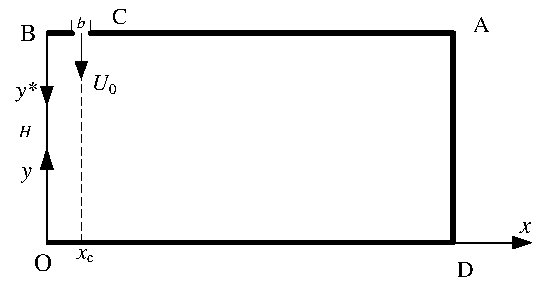
\includegraphics[width=\linewidth]{figs/zuobiaoxi.pdf}
	\caption{坐标系定义}
	\label{zuobiaoxi}
\end{figure}






\section{竖壁贴附区壁射流边界层分析}

拐角区使用中线势流假设，其余两个壁面是壁射流问题，使用相似解分析



\subsection{竖向壁面区的相似解分析}
引入射流型边界层假设以及流函数，坐标系为$y'O'x$，忽略法向$x$的动量方程。流向速度与法向速度分别为$u,v$.
\begin{align}
    u=\frac{\partial \psi}{\partial x}, \quad -v=\frac{\partial \psi}{\partial y'}
\end{align}
流向动量方程为：
\begin{align}
     \frac{\partial \psi}{\partial x}\frac{\partial^{2} \psi}{\partial y'\partial x} - \frac{\partial \psi}{\partial y'}\frac{\partial^{2} \psi}{\partial x^{2}}=\nu\frac{\partial^{3} \psi}{\partial x^{3}}
\end{align}

引入竖壁区的局部特征尺度$U_{1}(y'),L_{1}(y')$，相似解定义为：
\begin{align}
    \psi=U_{1}L_{1}f(\frac{x}{L_{1}}), \quad \eta_{1}=\frac{x}{L_{1}}
\end{align}

\begin{align}
    u=\frac{\partial \psi}{\partial x}&=U_{1}f'\\
    -v=\frac{\partial \psi}{\partial y'}&=f\left(
    L_{1}\frac{\mathrm{d}U_{1}}{\mathrm{d}y'}+U_{1}\frac{\mathrm{d}L_{1}}{\mathrm{d}y'}
    \right)-f'\frac{U_{1}x}{L_{1}}\frac{\mathrm{d}L_{1}}{\mathrm{d}y'}\\
    \frac{\partial u}{\partial y'}=\frac{\partial^{2} \psi}{\partial y'\partial x}&=f'\frac{\mathrm{d}U_{1}}{\mathrm{d}y'}-
    \frac{U_{1}x}{L_{1}^{2}}f''\frac{\mathrm{d}L_{1}}{\mathrm{d}y'}\\
    \frac{\partial u}{\partial x}=\frac{\partial^{2} \psi}{\partial x^{2}}&=\frac{U_{1}}{L_{1}}f''\\
    \frac{\partial^{2} u}{\partial x^{2}}=\frac{\partial^{3} \psi}{\partial x^{3}}&=\frac{U_{1}}{L_{1}^{2}}f'''
\end{align}

竖壁区的边界层流向动量方程为：
\begin{align}
    \label{eq-ode-v-wall}
    f'''+\left(\frac{L_{1}^{2}}{\nu}\frac{\mathrm{d}U_{1}}{\mathrm{d}y'}+\frac{L_{1}U_{1}}{\nu}\frac{\mathrm{d}L_{1}}{\mathrm{d}y'}\right)ff''-\frac{L_{1}^{2}}{\nu}\frac{\mathrm{d}U_{1}}{\mathrm{d}y'}f'f'=0
\end{align}

存在相似解的条件方程组为：
\begin{align}
    \frac{L_{1}^{2}}{\nu}\frac{\mathrm{d}U_{1}}{\mathrm{d}y'}&=a_{1}\\
    \frac{L_{1}U_{1}}{\nu}\frac{\mathrm{d}L_{1}}{\mathrm{d}y'}&=b_{1}
\end{align}
其中$a_{1},b_{1}$分别为常数。

式\ref{eq-ode-v-wall}写为
\begin{align}
    f'''+(a_{1}+b_{1})ff''-a_{1}f'f'=0
\end{align}

竖壁区壁射流边界条件为：
\begin{align}
    &0<y'<H_{s}\notag\\
    &x=0,\quad f=f'=0; \quad x\rightarrow \infty,\quad f'=0
\end{align}
其中$H_{s}$为竖壁区域射流入口到分离点的长度。

令$a_{1}+b_{1}=1$，则\ref{eq-ode-v-wall}可写为
\begin{align}
    f'''+ff''+(b_{1}-1)f'f'=0
\end{align}

引入守恒量求出$b_{1}$的值。

变形后的原始变量边界层控制方程
\begin{align}
    \rho u\frac{\partial u}{\partial y'}+\rho u\frac{\partial v}{\partial x}&=0\\
    \rho u\frac{\partial u}{\partial y'}+\rho v\frac{\partial u}{\partial x}&=\mu\frac{\partial^{2}u}{\partial x^{2}}
\end{align}

两式相加合并微分得到
\begin{align}
    \rho\left(\frac{\partial uu}{\partial y'}+\frac{\partial uv}{\partial x}\right)=\mu\frac{\partial^{2}u}{\partial x^{2}}=\frac{\partial \tau}{\partial x}
\end{align}
其中$\tau$表示流向的切应力。沿竖向区域的壁射流法向($x$方向)积分
\begin{align}
    \rho\frac{\mathrm{d}}{\mathrm{d}y'}\int_{0}^{\infty}uu\mathrm{d}x=-\tau_{w}\\
    \frac{\mathrm{d}J}{\mathrm{d}y'}=-\tau_{w}
\end{align}
上式表面在壁射流相似解成立的区域内，壁射流的动量通量沿流向与壁面切应力平衡，此时无法获得能求出相似ODE特征值的条件表达式。

在壁射流以内，壁面以上任一点$x$到壁射流外缘$x=\infty$上对壁射流边界层动量方程积分
\begin{align}
    \int_{x}^{\infty}\rho\left(\frac{\partial uu}{\partial y'}+\frac{\partial uv}{\partial x}\right)\mathrm{d}x=\int_{x}^{\infty}\frac{\partial \tau}{\partial x}\mathrm{d}x\\
    \frac{\partial }{\partial y'}\int_{x}^{\infty}\rho uu\mathrm{d}x-\rho uv|_{x}=-\tau_{x}
\end{align}

令$W=\int_{x}^{\infty}\rho uu\mathrm{d}x$，则有$\frac{\partial W}{\partial x}=-\rho uu$。上式变形为
\begin{align}
    \frac{\partial W}{\partial y'}-\rho uv|_{x}=-\tau_{x}\\
    u\frac{\partial W}{\partial y'}-u\rho uv|_{x}=-u\tau_{x}\\% 乘上一个积分起点处x的流向速度u
    u\frac{\partial W}{\partial y'}+v\frac{\partial W}{\partial x}+u\tau_{x}=0
\end{align}

引入两边同乘$W$的连续方程
\begin{align}
    W\frac{\partial u}{\partial y'}+W\frac{\partial v}{\partial x}=0
\end{align}

合并两个式子
\begin{align}
    \frac{\partial uW}{\partial y'}+\frac{\partial vW}{\partial x}+u\tau=0
\end{align}

沿竖向区域的壁射流法向($x$方向)积分
\begin{align}
    \int_{0}^{\infty}\frac{\partial uW}{\partial y'}\mathrm{d}x+\int_{0}^{\infty}\frac{\partial vW}{\partial x}\mathrm{d}x+\int_{0}^{\infty}u\tau\mathrm{d}x=0\\
    \frac{\partial }{\partial y'}\int_{0}^{\infty}uW\mathrm{d}x+vW|_{0}^{\infty}+\int_{0}^{\infty}u\tau\mathrm{d}x=0
\end{align}
边界条件：$W(\infty)=0，\quad v(0)=0$
\begin{align}
    \frac{\partial }{\partial y'}\int_{0}^{\infty}uW\mathrm{d}x+\mu\int_{0}^{\infty}\frac{\partial \frac{u^{2}}{2}}{\partial x}\mathrm{d}x=0\\
    \frac{\mathrm{d} }{\mathrm{d} y'}\int_{0}^{\infty}uW\mathrm{d}x=0
\end{align}
得到守恒量：
\begin{align}
    F=\int_{0}^{\infty}u\left(\int_{x'}^{\infty}\rho uu\mathrm{d}x'\right)\mathrm{d}x=\cst
\end{align}
代入相似形式的量
\begin{align}
    \rho U_{1}^{3}L_{1}^{2}\int_{0}^{\infty}f'\left(\int_{\eta_{1}}^{\infty}f'f'\mathrm{d}\eta_{1}'\right)\mathrm{d}\eta_{1}=\cst
\end{align}
这个式子是壁射流相似解存在的条件方程，需要有
\begin{align}
    U_{1}^{3}L_{1}^{2}=\cst\\
    U_{1}^{2}L_{1}\left(2U_{1}\frac{\mathrm{d}L_{1}}{\mathrm{d}y'}+3L_{1}\frac{\mathrm{d}U_{1}}{\mathrm{d}y'}\right)=0
\end{align}
代入前两个条件方程：
\begin{align}
    a_{1}&=-2\\
    b_{1}&=3
\end{align}

最终得到了竖壁区壁射流相似解的数学表达式为：
\begin{align}
    &f'''+ff''+2f'f'=0\\
    \text{边界条件为：}\notag\\
     &0<y'<H_{s}\notag\\
    &x=0,\quad f=f'=0; \quad x\rightarrow \infty,\quad f'=0
\end{align}

\subsection{特征尺度表达式的推导}
解如下方程组
\begin{align}
    \frac{L_{1}^{2}}{\nu}\frac{\mathrm{d}U_{1}}{\mathrm{d}y'}&=-2\\
    \frac{L_{1}U_{1}}{\nu}\frac{\mathrm{d}L_{1}}{\mathrm{d}y'}&=3
\end{align}

令$P=\frac{\mathrm{d}U_{1}}{\mathrm{d}y'}$，由链式法则$\frac{\mathrm{d}L_{1}}{\mathrm{d}y'}=\frac{\mathrm{d}L_{1}}{\mathrm{d}P}\frac{\mathrm{d}P}{\mathrm{d}y'}$，以及$\frac{\mathrm{d}P}{\mathrm{d}y'}=\frac{\mathrm{d}P}{\mathrm{d}U_{1}}\frac{\mathrm{d}U_{1}}{\mathrm{d}y'}=\frac{\mathrm{d}P}{\mathrm{d}U_{1}}P$。

由原方程组第一式得：
\begin{align}
    L_{1}=\left(\frac{-2\nu}{P}\right)^{\frac{1}{2}}\\
    \frac{\mathrm{d}L_{1}}{\mathrm{d}P}=\frac{\nu}{P^{2}\sqrt{\frac{-2\nu}{P}}}\\
    \frac{\mathrm{d}L_{1}}{\mathrm{d}y'}=\frac{\nu}{P^{2}\sqrt{\frac{-2\nu}{P}}}\frac{\mathrm{d}^{2}U_{1}}{\mathrm{d}y'^{2}}
\end{align}

由原方程组第二式得：
\begin{align}
    \frac{U_{1}}{P^{2}}\frac{\mathrm{d}^{2}U_{1}}{\mathrm{d}y'^{2}}=3\\
    \frac{U_{1}}{P^{2}}\frac{\mathrm{d}P}{\mathrm{d}y'}=3\\
    \frac{\mathrm{d}P}{\mathrm{d}y'}=\frac{3P^{2}}{U_{1}}\\
    \frac{\mathrm{d}P}{3P}=\frac{\mathrm{d}U_{1}}{U_{1}} \\% 代入了第二个链式法则公式
    P=\frac{\mathrm{d}U_{1}}{\mathrm{d}y'}=C_{1}U_{1}^{3}\\
    U_{1}=\left(\frac{-1}{2(C_{1}y'+C_{2})}\right)^{\frac{1}{2}}
\end{align}

回代求$L_{1}$
\begin{align}
    L_{1}&=\sqrt{\frac{-2\nu}{C_{1}}}U_{1}^{-\frac{3}{2}}\\
        &=\sqrt{\frac{-2\nu}{C_{1}}}\left(\frac{-1}{2(C_{1}y'+C_{2})}\right)^{-\frac{3}{4}}
\end{align}

为了确定两个积分常数$C_{1},C_{2}$，引入物理边界条件假设：射流入口平均速度为$U_{0}$，取入口中心轴线处$x=\frac{B}{2},u(0,\frac{B}{2})=U_{0}$，壁射流最大流速所在的轴线也是由此开始，且由于速度衰减，从出口往后的最大速度也不会超过$U_{0}$，由前面的相似解表达式有：
\begin{align}
    u(0,\frac{B}{2})=U_{1}(0)f'(\frac{B}{2L_{1}(0)})=U_{0}
\end{align}
令此时相似变量描述的就是速度剖面中最大速度的位置，即$\eta_{m}=\frac{B}{2L_{1}(0)},f'_{m}=f'(\eta_{m})$，那么有：
\begin{align}
    L_{1}(0)&=\frac{B}{2\eta_{m}}\\
    U_{1}(0)&=\frac{U_{0}}{f'_{m}}
\end{align}

将上面两式左边代入$U_{1},L_{1}$的原始表达式：
\begin{align}
    \sqrt{\frac{-1}{2C_{2}}}&=\frac{U_{0}}{f'_{m}}\\
    \sqrt{\frac{-2\nu}{C_{1}}}U_{1}^{-\frac{3}{2}}(0)&=\frac{B}{2\eta_{m}}
\end{align}
解得积分常数$C_{1},C_{2}$：
\begin{align}
    C_{1}&=\frac{-8\nu \eta_{m}^{2}f_{m}^{'3}}{B^{2}U_{0}^{3}}\\
    C_{2}&=\frac{-f'^{2}_{m}}{2U_{0}^{2}}
\end{align}

则特征尺度显式表达式：
\begin{align}
    U_{1}(y')&=\frac{BU_{0}^{\frac{3}{2}}}{f'_{m}(16\nu \eta^{2}_{m}f'_{m}y'-B^{2}U_{0})^{1/2}}\\
    L_{1}(y')&=\frac{1}{2\eta_{m}B^{\frac{1}{2}}}\left(\frac{16\nu \eta^{2}_{m}f'_{m}y'-B^{2}U_{0}}{U_{0}f'_{m}}\right)^{\frac{3}{4}}
\end{align}

用射流出口宽度$B$归一化的特征尺度表达式：
\begin{align}
    Y_{b}&=\frac{y'}{B}\\
    U_{1}(Y_{b})&=\frac{BU_{0}^{\frac{3}{2}}}{f'_{m}(16\nu \eta^{2}_{m}f'_{m}BY_{b}-B^{2}U_{0})^{1/2}}\\
    L_{1}(Y_{b})&=\frac{1}{2\eta_{m}B^{\frac{1}{2}}}\left(\frac{16\nu \eta^{2}_{m}f'_{m}BY_{b}-B^{2}U_{0}}{U_{0}f'_{m}}\right)^{\frac{3}{4}}
\end{align}

\subsection{竖壁区特征量的推导}
\discard{
\subsubsection*{壁射流断面平均流速流向分布}
定义壁射流在 $y'$ 截面的平均流速为：
\begin{align}
    u_a(y') = \frac{1}{\delta(y')}\int_0^{\delta(y')} u(y', x) \, \mathrm{d}x
\end{align}

其中 $\delta(y')$ 表示该截面上的壁射流厚度。

代入相似解形式：
\begin{align}
    u(y', x) = U_1(y') f'\left( \frac{x}{L_1(y')} \right)
\end{align}

进行变量代换 $x = \eta L_1(y')$，得：
\begin{align}
    Q(y') &= \int_0^{\delta(y')} u(y', x) \, \mathrm{d}x = U_1(y') L_1(y') \int_0^{\eta_\infty} f'(\eta) \, \mathrm{d}\eta \\
          &= U_1(y') L_1(y') Q^*
\end{align}

其中定义归一化常数：
\begin{align}
    Q^* = \int_0^{\eta_\infty} f'(\eta) \, \mathrm{d}\eta
\end{align}

由于 $\delta(y') = L_1(y') \eta_\infty$，故有：
\begin{align}
    u_a(y') &= \frac{Q(y')}{\delta(y')} 
    = \frac{U_1(y') L_1(y') Q^*}{L_1(y') \eta_\infty} 
    = \left( \frac{Q^*}{\eta_\infty} \right) U_1(y')
\end{align}

从而得出平均速度与局部速度尺度成正比：
\begin{align}
    u_a(y') = C_a \cdot U_1(y'), \quad C_a = \frac{Q^*}{\eta_\infty}
\end{align}

\subsubsection*{断面速度分布}
速度分布归一化表达为：
\begin{align}
    \frac{u(y',x)}{u_{m}(y',x_{m})}=\frac{f'(\eta)}{f'(\eta_{m})}=g(\frac{x}{x_{m}})
\end{align}
\begin{itemize}
    \item $x_{m}=\eta_{m}L_{1}(y')$为最大速度所对应的横向位置
    \item $f'(\eta)$为相似解的数值解
    \item 此归一化分布为普适曲线，与系统参数$B,U_{0}$等无关
\end{itemize}
该表达式可通过数值解相似ODE后归一化绘图得到。

}
%%%%%%%%%%%%%%%%%%%%%%%%%%%%%%%%%%%%%%%%%%%%%%%%%%%%%%
\subsubsection{壁射流守恒量}

壁射流相似结构成立的特征守恒量 $F$，其物理意义为沿流向的动量扩散势的通量守恒。

定义式为：
\begin{align*}
    F &= \rho U_{1}^{3}L_{1}^{2} \int_{0}^{\infty}f'\left(\int_{\eta_{1}}^{\infty}f'f'\,\mathrm{d}\eta_{1}'\right)\,\mathrm{d}\eta_{1}
    = \rho U_{1}^{3}L_{1}^{2}F^{*} = \text{const}
\end{align*}
其中 $F^*$ 为无量纲动量结构因子，是由相似解唯一确定的常数。

$F$ 的物理维度为 $[\mathrm{kg}\cdot\mathrm{m}/\mathrm{s}^3]$，表示单位宽度上单位时间内动量平方的沿流向扩散通量。在自相似结构成立的前提下，该量在流向保持恒定。

代入特征尺度表达式得到：
\begin{align}
    U_{1}^{3}L_{1}^{2} = \frac{B^{2}U_{0}^{3}}{4\eta_{m}^{2}f_{m}^{'\frac{9}{2}}}
\end{align}

数值计算无量纲常数：
\begin{align}
    F^{*} = \int_{0}^{\infty}f'\left(\int_{\eta_{1}}^{\infty}f'f'\,\mathrm{d}\eta_{1}'\right)\,\mathrm{d}\eta_{1} = 0.100054
\end{align}

因此，壁射流的特征守恒量最终表达式为：
\begin{align}
    F = 0.100054\cdot \frac{\rho B^{2}U_{0}^{3}}{4\eta_{m}^{2}f_{m}^{'\frac{9}{2}}}
\end{align}


\subsubsection{壁射流壁面切应力流向分布}
切应力及壁面切应力定义为:
\begin{align*}
    \tau&=\mu\frac{\partial u}{\partial x}\\
    \tau_{w}&=\mu\frac{\partial u}{\partial x}|_{x=0}
\end{align*}

代入相似解表达式：
\begin{align}
    \tau_{w}=\mu\frac{U_{1}}{L_{1}}f''(0)
\end{align}

使用射流出口参数$U_{0},B$对切应力以及流向坐标$y'$进行无量纲化，表达式为：
\begin{align}
    \frac{\tau_{w}}{\mu\frac{U_{0}}{B}}=\frac{2\eta_{m}f''(0)(BU_{0})^{\frac{5}{4}}}{f_{m}^{'\frac{1}{4}}(16\nu\eta_{m}^{2}f'_{m}\frac{y'}{B}-BU_{0})^{\frac{5}{4}}}
\end{align}

\subsubsection{壁射流最大速度及法向速度流向分布}

壁射流的流向速度满足如下相似解形式：
\begin{align*}
    u(y',x) = U_{1}(y')\,f'\left(\frac{x}{L_{1}(y')}\right)
\end{align*}

定义每个法向位置 $y'$ 上的最大速度为 $u_{m}(y')$，其对应的位置为 $x = x_{m}(y')$，使得：
\begin{align*}
    u_{m}(y') = u(y', x_{m}) = U_{1}(y')\,f'\left(\frac{x_{m}}{L_{1}(y')}\right)
    = U_{1}(y') f'_{m}, \quad \text{其中}\quad \eta_{m} = \frac{x_{m}}{L_{1}(y')}
\end{align*}

代入 $U_{1}(y')$ 的显式表达式，可得最大速度相对于出口平均速度 $U_{0}$ 的无量纲流向分布：
\begin{align}
    \frac{u_{m}(y')}{U_{0}} &= \frac{B\,U_{0}^{1/2}}{\left(16\nu\,\eta^{2}_{m}f'_{m}y' - B^{2}U_{0}\right)^{1/2}} \notag \\
    &= \left( \frac{16\nu\,\eta_{m}^{2}f'_{m}}{B U_{0}} \frac{y'}{B} - 1 \right)^{-1/2} \notag \\
    &= \left( \frac{16\nu\,\eta_{m}^{2}f'_{m}}{B U_{0}} Y_{b} - 1 \right)^{-1/2} \label{eq:um_dist}
\end{align}
该式描述了壁射流随下游方向的速度衰减规律。

\vspace{0.5em}
壁射流的法向速度分量由相似解导出为：
\begin{align*}
    v(y', x) = f'\frac{U_{1}(y')x}{L_{1}(y')} \frac{\mathrm{d}L_{1}}{\mathrm{d}y'} - f\left(\frac{x}{L_{1}(y')}\right) \frac{\mathrm{d}}{\mathrm{d}y'}\left[U_{1}(y')L_{1}(y')\right]
\end{align*}

特别地，考虑最大速度所在的流线 $x = x_{m}(y')$，其对应的法向速度定义为 $v_{m}(y')$，可写为：
\begin{align*}
    v_{m}(y') = f'_{m}\,\eta_{m}\,U_{1}(y')\,\frac{\mathrm{d}L_{1}}{\mathrm{d}y'}
    - f_{m}\,\frac{\mathrm{d}}{\mathrm{d}y'}\left[ U_{1}(y')\,L_{1}(y') \right]
\end{align*}
其中 $f'_{m} = f'(\eta_{m})$，$f_{m} = f(\eta_{m})$ 为相似函数在 $\eta_{m}$ 处的取值。

将 $U_1, L_1$ 的显式表达式代入，并进行无量纲化，得到 $v_{m}/U_{0}$ 的表达式为：
\begin{align}
    \frac{v_{m}}{U_{0}} = \frac{16\nu\,\eta^{2}_{m}f'_{m}}{B^{1/4}U_{0}^{1/4}f_{m}^{'3/4}(16\nu\,\eta^{2}_{m}f'_{m}Y_{b}-BU_{0})^{3/4}}\left(\frac{3}{8}+\frac{f_{m}}{8\eta_{m}f'_{m}B^{1/2}(16\nu\,\eta^{2}_{m}f'_{m}Y_{b}-BU_{0})^{1/2}}\right)
    \label{eq:vm}
\end{align}

公式 \eqref{eq:um_dist} 与 \eqref{eq:vm} 分别描述了壁射流沿流向的流向最大速度与特征轴线上的法向速度演化趋势。




\subsubsection{特征厚度参数}
定义一组描述壁射流剖面结构的典型厚度度量

\begin{enumerate}
    \item 内层厚度$\delta_{m}$
    \begin{align*}
        \delta_{m}&=L_{1}(y')\eta_{m}\\
        &=\frac{1}{2B^{\frac{1}{2}}}\left(\frac{16\nu\eta_{m}^{2}f'_{m}y'-B^{2}U_{0}}{U_{0}f'_{m}}\right)^{\frac{3}{4}}
    \end{align*}
    表示最大速度出现的位置与壁面的距离，通常是壁射流内层的厚度。

使用射流出口宽度$B$进行无量纲化：
\begin{align}
    \frac{\delta_{m}}{B}&=\frac{1}{2}\left(\frac{16\nu\eta_{m}^{2}f'_{m}Y_{b}-BU_{0}}{BU_{0}f'_{m}}\right)^{\frac{3}{4}}\\
    &=g(Y_{b})
\end{align}
    \item 特征厚度$\delta_{0.5}$：$u=0.5u_{m}$所在的法向坐标位置，定义为
    \begin{align*}
        \delta_{0.5}&=\delta_{m}+L_{1}(y')\eta_{0.5}\\
        &=L_{1}(\eta_{m}+\eta_{0.5})\\
        &=\frac{1}{2\eta_{m}B^{\frac{1}{2}}}\left(\frac{16\nu\eta_{m}^{2}f'_{m}y'-B^{2}U_{0}}{U_{0}f'_{m}}\right)^{\frac{3}{4}}(\eta_{m}+\eta_{0.5})
    \end{align*}
    其中，$\eta_{0.5}$由$f'(\eta_{0.5})=0.5f'_{m}$数值反解，可通过插值法获得。
    
    使用射流出口宽度$B$进行无量纲化
    \begin{align}
        \frac{\delta_{0.5}}{B}=\frac{1}{2\eta_{m}B^{\frac{3}{4}}}\left(\frac{16\nu\eta_{m}^{2}f'_{m}Y_{b}-BU_{0}}{U_{0}f'_{m}}\right)^{\frac{3}{4}}(\eta_{m}+\eta_{0.5})
    \end{align}
    \item 外缘厚度$\delta$：定义为射流速度接近0的法向坐标位置，表示的是射流的全厚度。
    \begin{align*}
        \delta&=L_{1}(y')\eta_{\infty}\\
        &=\frac{1}{2\eta_{m}B^{\frac{1}{2}}}\left(\frac{16\nu\eta_{m}^{2}f'_{m}y'-B^{2}U_{0}}{U_{0}f'_{m}}\right)^{\frac{3}{4}}\eta_{\infty}
    \end{align*}
    通常选取$\eta_{\infty}\approx 6\sim10$即可满足工程精度，本研究中最大取到了12.
    使用射流出口宽度$B$进行无量纲化
    \begin{align}
        \frac{\delta}{B}=\frac{1}{2\eta_{m}B^{\frac{3}{4}}}\left(\frac{16\nu\eta_{m}^{2}f'_{m}Y_{b}-BU_{0}}{U_{0}f'_{m}}\right)^{\frac{3}{4}}\eta_{\infty}
    \end{align}
\end{enumerate}

\subsubsection{壁射流外缘法向速度沿流向分布}
法向速度分量的相似解形式为：
\begin{align*}
    v=f'\frac{U_{1}x}{L_{1}}\frac{\mathrm{d}L_{1}}{\mathrm{d}y'}-f\frac{\mathrm{d}U_{1}L_{1}}{\mathrm{d}y'}
\end{align*}

由于 $\eta \to \infty$ 处的速度函数趋于常数，故在理论表达中无法直接带入无穷。为处理该问题，引入数值截断点 $\eta_\infty$ 作为边界层外缘的近似位置。根据相似结构，有：

\[
v_{\infty}(y') \approx f'(\eta_\infty) \cdot U_1(y') \cdot \eta_\infty \cdot \frac{dL_1}{dy'} - f(\eta_\infty) \cdot \frac{d(U_1 L_1)}{dy'}
\]

其中 $\eta_\infty$ 可取 $10\sim12$，具体由数值计算确定。

这里我们根据前面的分析与数值结果取值为：
\[
\eta_{\infty}=12, \quad f(\infty)=1, \quad f'(\infty)=0
\]

则外缘法向速度表达式变为
\begin{align*}
    v_{\infty}&=-\frac{\mathrm{d}(U_{1}L_{1})}{\mathrm{d}y'}\\
    &=\frac{16\nu\eta_{m}^{2}f'_{m}B^{\frac{1}{2}}U_{0}^{\frac{3}{4}}}{8\eta_{m}f_{m}^{'\frac{7}{4}}(16\nu\eta_{m}^{2}f'_{m}y'-B^{2}U_{0})^{\frac{5}{4}}}
\end{align*}

使用射流出口流速和宽度进行无量纲化
\begin{align}
    \frac{v_{\infty}}{U_{0}}&=\frac{16\nu\eta_{m}^{2}f'_{m}}{8\eta_{m}f_{m}^{'\frac{7}{4}}B^{\frac{3}{4}}U_{0}^{\frac{1}{4}}(16\nu\eta_{m}^{2}f'_{m}Y_{b}-BU_{0})^{\frac{5}{4}}}\\
    & = g(Y_{b})
\end{align}

\subsubsection{壁射流体积通量沿流向分布}
壁射流在$y'$截面的流量为
\begin{align*}
    Q(y')=\int_{0}^{\delta(y')}u(y',x)\mathrm{d}x=U_{1}(y')L_{1}(y')\int_{0}^{\eta_{\infty}}f'\mathrm{d}\eta
\end{align*}
定义归一化常数：
\begin{align*}
    Q^{*}=\int_{0}^{\eta_{\infty}}f'\mathrm{d}\eta
\end{align*}
其中$Q^{*}$由相似解确定，与系统参数无关。

断面流量$Q=Q^{*}U_{1}L_{1}$，该量可用于描述断面体积流量随流向的演化。

考虑使用射流出口平均速度$U_{0}$与出口宽度$B$的乘积作为归一化特征流量，则断面归一化体积流量为：
\begin{align}
    \frac{Q}{Q_{0}}&=Q^{*}\frac{U_{1}(Y_{b})}{U_{0}}\frac{L_{1}(Y_{b})}{B}\\
    &=\frac{Q^{*}(16\nu\eta_{m}^{2}f'_{m}Y_{b}-BU_{0})^{\frac{1}{4}}}{2\eta_{m}(BU_{0})^{\frac{1}{4}}f_{m}^{'\frac{7}{4}}}\\
    &=g(Y_{b})
\end{align}

\subsubsection{壁射流动量通量沿流向分布}
壁射流在$y'$截面的动量通量为
\begin{align*}
    K(y')=U_{1}L_{1}\int_{0}^{\eta_{\infty}}f'^{2}\mathrm{d}\eta
\end{align*}

定义归一化常数
\begin{align*}
    K^{*}=\int_{0}^{\eta_{\infty}}f'^{2}\mathrm{d}\eta
\end{align*}
其中$K^{*}$由相似解确定，与系统参数无关。

断面动量通量$K=K^{*}U_{1}^{2}L_{1}$，该量可用于描述断面动量通量随流向的演化。

考虑使用射流出口平均速度$U_{0}$与出口宽度$B$作为归一化特征参量，则断面归一化动量通量为：
\begin{align}
    \frac{K}{K_{0}}&=K^{*}\frac{U_{1}^{2}(Y_{b})}{U_{0}^{2}}\frac{L_{1}(Y_{b})}{B}\\
    &=\frac{Q^{*}(16\nu\eta_{m}^{2}f'_{m}Y_{b}-BU_{0})^{\frac{1}{4}}}{2\eta_{m}(BU_{0})^{\frac{1}{4}}f_{m}^{'\frac{7}{4}}}\\
    &=g(Y_{b})
\end{align}

\subsubsection{壁射流核心区持续长度}
直觉感觉很短

\subsubsection{贴附距离}
贴附距离$H_{s}$是指壁射流相似结构在流向上保持的末端位置，通常有如下的物理判据：
\begin{enumerate}
    \item 壁面切应力流向的导数为0
    \begin{align*}
        \frac{\mathrm{d}\tau_{w}}{\mathrm{d}y'}|_{y'=H_{s}}=0,\quad \tau_{w}=\mu\frac{\partial u}{\partial x}|_{x=0}
    \end{align*}
    该判据表示壁面剪切效应减弱至极小，意味着壁射流边界层与壁面分离。
    \item 最大速度流向的导数为0
    \begin{align*}
        \frac{\mathrm{d}u_{m}}{\mathrm{d}y'}|_{y'=H_{s}}=0
    \end{align*}
    表示壁射流中心轴线速度达到极小值以后可能出现回流或失稳。
\end{enumerate}
数值上可以通过拟合$u_{m}(y')$曲线，计算其导数并寻找零点位置获得$H_{s}$。

\paragraph{(1)注记}
分离点不单单取决于上游的壁射流流动，还取决于下游拐角区的回流涡的流动特性，因此需要将两个部分的流动模型都建立完成后，在分离点处匹配得出具体的分离点坐标位置。








 % 竖壁壁射流边界层分析

%\section{守恒量引导的内禀尺度}
\subsection{守恒量的推导}
存在压力梯度的壁射流动量方程：
\begin{align}
    \frac{\partial uu}{\partial x}+\frac{\partial uv}{\partial y}=-\frac{1}{\rho}\frac{\partial p}{\partial x}+\nu\frac{\partial^{2} u}{\partial y^{2}}=-\frac{1}{\rho}\frac{\partial p}{\partial x}+\frac{1}{\rho}\frac{\partial\tau}{\partial y}
\end{align}
边界条件：
\begin{align}
    y=0,x>0&:\quad \psi=u=v=0\\
    y\rightarrow \infty，x>0&: \quad \tau=u=0
\end{align}

对动量方程从壁面法向某一点$y'$至$\infty$积分：
\begin{align}
    \int_{y'}^{\infty}\rho(\frac{\partial uu}{\partial x}+\frac{\partial uv}{\partial y})\mathrm{d}y'&=\int_{y'}^{\infty}\frac{\partial\tau}{\partial y}-\frac{\partial p}{\partial x}\mathrm{d}y'\\
    \frac{\partial}{\partial x}\rho\int_{y'}^{\infty}uu\mathrm{d}y'+\frac{\partial }{\partial x}\int_{y'}^{\infty}p\mathrm{d}y'-\rho uv&=-\tau
\end{align}

令$W=\int_{y'}^{\infty}(\rho uu+p)\mathrm{d}y'$，且有$\frac{\partial W}{\partial y}=-\rho uu-p$:
\begin{align}
    \frac{\partial W}{\partial x}-\rho uv+\tau=0
\end{align}
上式两边乘以$u$，与流场耦合
\begin{align}
     u\frac{\partial W}{\partial x}-\rho uuv+u\tau=0\\
     u\frac{\partial W}{\partial x}+v\frac{\partial W}{\partial y}+vp+u\tau=0
\end{align}
上面的式子描述了物理量$W$的对流输运。

将连续方程两边乘以$W$再加到上面的式子中：
\begin{align}
    W\frac{\partial u}{\partial x}+W\frac{\partial v}{\partial y}=0\\
    u\frac{\partial W}{\partial x}+v\frac{\partial W}{\partial y}+u\tau+vp+W\frac{\partial u}{\partial x}+W\frac{\partial v}{\partial y}=0\\
    \frac{\partial uW}{\partial x}+\frac{\partial vW}{\partial y}+vp+u\tau=0
\end{align}
如果补充非定常项:
\begin{align}
    \frac{\partial W}{\partial t}+\frac{\partial uW}{\partial x}+\frac{\partial vW}{\partial y}+vp+u\tau=0\\
    \frac{\mathrm{D}W}{\mathrm{D}t}+vp+u\tau=0
\end{align}
上式表明，广义机械能通量势（Generalized Mechanical Energy Potential）$W$ 的随体变化由两个机制驱动：一是主流速度 $u$与切应力 $\tau$ 的耦合作用，即壁面摩擦对流体的做功；二是压强通过法向速度 $v$ 所进行的功，即压强在法向上的作用，这项 $vp$ 描述了单位体积上由于压力梯度作用导致垂向流动所引入的压强功，是动量结构沿流向演化的重要推动因子。这个量描述了：壁射流中压力梯度+动量输运对局部能量结构的耦合控制机制

至此讨论的是在壁射流区域中某点$y$往上积分所得到的广义机械能通量势的输运方程

对上式在$y$方向上，从0至$\infty$积分：
\begin{align}
    \int_{0}^{\infty}\frac{\partial uW}{\partial x}\mathrm{d}y
    +\int_{0}^{\infty}\frac{\partial vW}{\partial y}\mathrm{d}y
    +\int_{0}^{\infty}(vp+u\tau)\mathrm{d}y=0
\end{align}
代入边界条件，最后得到：
\begin{align}
    \frac{\mathrm{d}}{\mathrm{d}x}\int_{0}^{\infty}uW\mathrm{d}y+\int_{0}^{\infty}vp\mathrm{d}y=0
\end{align}
假设：
\begin{align}
    \frac{\mathrm{d}Q}{\mathrm{d}x}=\int_{0}^{\infty}vp\mathrm{d}y
\end{align}
则有
\begin{align}
    \frac{\mathrm{d}}{\mathrm{d}x}\left(\int_{0}^{\infty}uW\mathrm{d}y+Q\right)=0
\end{align}
这表明：
\begin{align}
    \int_{0}^{\infty}uW\mathrm{d}y+Q=\int_{0}^{\infty}u\left(\int_{y'}^{\infty}(\rho uu+p)\mathrm{d}y'\right)\mathrm{d}y+Q=F=\cst
\end{align}
这说明在壁射流问题中$F$是一个守恒量。

\subsection{如何确定\(Q\)的具体表达式}

假设壁射流中最大流向速度所在的流线为势流，在此流线上引入Bernoulli方程重建压力梯度。

若最大速度所在的流线为 \(y = y_m(x)\)，从射流起点到该流线上任意一点有如下关系：
\begin{align}
    \frac{1}{2}u_m^2 + \frac{p(x, y_m)}{\rho} = \text{常数} \\
    \frac{\partial p(x, y_m)}{\partial x} = -\rho u_m \frac{\mathrm{d} u_m}{\mathrm{d} x}
\end{align}

假设：壁射流中压力的主要流向变化主要由射流中心（最大速度位置，记为 \(y = y_m(x)\)）上的压强分布主导，即
\begin{align}
    \frac{\partial p(x, y)}{\partial x} \approx \frac{\partial p(x, y_m)}{\partial x}
\end{align}

代入上一节的推导过程，有：
\begin{align}
    \frac{\mathrm{d}}{\mathrm{d}x} \int_0^\infty uW\,\mathrm{d}y - \int_0^\infty v\frac{u_m^2}{2}\,\mathrm{d}y = 0
\end{align}

记垂向体积流率：
\begin{align}
    V_i(x) = \int_0^\infty v\,\mathrm{d}y
\end{align}

于是：
\begin{align}
    \frac{\mathrm{d}Q}{\mathrm{d}x} = -\int_0^\infty v\frac{u_m^2}{2}\,\mathrm{d}y = -\frac{u_m^2(x)}{2} V_i(x)
\end{align}

这说明压力梯度项的贡献，可以以最大速度平方乘以垂向体积流率的形式体现。

该项 \( Q(x) \) 的物理意义在于：

\begin{itemize}
    \item 它表征了由于流向压力梯度的存在，使得射流流线在靠近壁面的区域发生法向弯折，从而形成非零的法向速度 \( v \)；
    \item 其中 \( u_m^2/2 \) 是射流中心处的动能密度，而 \( V_i(x) = \int_0^\infty v\,dy \) 描述了这一法向弯折趋势的强弱，反映了法向流动的整体量级；
    \item 因此，\( Q \sim \frac{u_m^2}{2} V_i \) 表示压力梯度引起的轴向动能通过法向速度发生“再分布”的程度，可视为压力梯度引导下流动结构的变化量。
\end{itemize}

该项对壁射流的流动特性具有重要影响：

\begin{enumerate}
    \item \textbf{调控自相似结构的扩展：}若 \( Q \) 项较大，说明法向偏折效应显著，主流动量需要通过更宽广的流动区域维持，从而导致射流更强烈地扩展；
    
    \item \textbf{改变最大速度 \( u_m(x) \) 的衰减速率：}\( Q \) 的存在抑制了 \( u_m \) 的快速衰减。在压力梯度作用下，经典的 \( u_m \sim x^{-a} \) 的幂律结构将受到改动，以维持整体动量守恒；
    
    \item \textbf{预测流动分离：}在逆压梯度（\( \mathrm{d}p/\mathrm{d}x > 0 \)）条件下，若 \( Q \) 增长速度超过动量扩散项增长，可能导致 \( \frac{\mathrm{d}}{\mathrm{d}x}F_{\text{eff}} < 0 \)，破坏自相似守恒结构，从而导致局部分离或回流；
    
    \item \textbf{扩展动量守恒形式：}传统动量积分中使用动量厚度项 \( \int uu\,dy \)，而在包含压力梯度的情形中，引入 \( Q \) 后的总动量守恒形式为：
    \[
        \frac{\mathrm{d}}{\mathrm{d}x} \left[ \int_0^\infty uW\,\mathrm{d}y + Q(x) \right] = 0
    \]
    这表明：总动量的守恒由剪切项与压力引导的动能转化项共同维护，为壁射流提供了更合理的物理描述。
\end{enumerate}

因此，\( Q \) 项在包含压力梯度的壁射流问题中不可忽略，它不仅提供了动能注入的来源，还决定了壁射流的扩展、速度衰减及是否产生分离的关键特征。



\subsection{壁射流问题中的内禀尺度}
一般的黏性流体问题中，至少存在两个守恒量，分别是$\rho$和$\mu$。根据上一小节的推导发现$F$是壁射流问题中特有的守恒量。现在我们使用这个三个守恒量重新构建壁射流的内禀尺度$\mathrm{U}$、$\mathrm{L}$，可以被用来确定壁射流相似解的具体形式。

壁射流守恒量的量纲表示为：
\begin{align}
    [F]&=\frac{\mathrm{ML^{2}}}{\mathrm{T}^{3}}\\
    [\rho]&=\frac{\mathrm{M}}{\mathrm{L^{3}}}\\
    [\mu]&=\frac{\mathrm{M}}{\mathrm{LT}}
\end{align}
上式中$\mathrm{M}$、$\mathrm{L}$、$\mathrm{T}$分别代表质量、长度、时间量纲。

现在用守恒量来表示这些基本量纲，然后用基本量纲来表示内禀尺度$\mathrm{U}$、$\mathrm{L}$。

基本量纲表示为：
\begin{align}
    \mathrm{M}&=\frac{\rho^{4}\nu^{9}}{F^{3}}\\
    \mathrm{L}&=\frac{\rho\nu^{3}}{F}\\
    \mathrm{T}&=\frac{\rho^{2}\nu^{5}}{F^{2}}
\end{align}

内禀尺度$U$、$L$的量纲分别为
\begin{align}
    [U]&=\frac{\mathrm{L}}{\mathrm{T}}\\
    [L]&=\mathrm{L}
\end{align}
用守恒量表示为：
\begin{align}
    U=\frac{F}{\rho\nu^{2}}\\
    L=\frac{\rho\nu^{3}}{F}
\end{align}

特征长度、特征速度、黏性系数组成的无量纲数表示为：
\begin{align}
    \frac{UL}{\nu}=1
\end{align}
代入以后发现满足这个无量纲数。 % 守恒量推导内禀尺度
%
\subsection*{壁射流的特征量分析与幂律形式的合理性}

壁射流（laminar wall jet）问题中，经典的自相似分析方法依赖于一组适当的特征尺度来将偏微分方程简化为常微分方程。虽然文献中往往直接引入幂律形式的流函数 ansatz（如式(10.4)），但实际上这一 ansatz 的幂指数应来源于对积分不变量和尺度分析的系统推导。

本文在此完整整理这一推导过程，说明幂律结构的物理与数学基础。

\paragraph{(1) 问题背景与积分不变量}

壁射流问题中的控制方程为边界层近似下的二维不可压粘性流动方程，其关键积分不变量为：

\begin{equation}
F=\rho\int_{0}^{\infty}u\left(\int_{y}^{\infty}uu\mathrm{d}y'\right)\mathrm{d}y = \text{常数},
\end{equation}

其中 \( u(x,y) \) 为沿壁面的流向速度。该不变量表示单位长度沿壁方向上的动量扩散势通量保持不变。我们期望利用该不变量推导出特征速度 \( U(x) \) 与特征长度 \( L(x) \) 随下游坐标 \( x \) 的变化规律。

\paragraph{(2) 特征量假设与量纲平衡}

设特征速度和特征长度分别满足幂律形式：

\begin{equation}
U(x) \sim x^p, \quad L(x) \sim x^q.
\end{equation}

则积分不变量可写为：

\begin{equation}
F \sim \rho U^3 L^2 \sim \rho x^{3p + 2q}.
\end{equation}

由 \( F \) 为常数可得约束条件：

\begin{equation}
3p + 2q = 0. \tag{A}
\end{equation}

另一方面，动量方程中的主导项为：

\begin{equation}
u \frac{\partial u}{\partial x} \sim \nu \frac{\partial^2 u}{\partial y^2}
\Rightarrow \frac{U^2}{x} \sim \nu \frac{U}{L^2},
\end{equation}

即：

\begin{equation}
U \sim \frac{\nu x}{L^2} \Rightarrow x^p \sim \frac{\nu x}{x^{2q}} \Rightarrow p = 1 - 2q. \tag{B}
\end{equation}

联立(A)、(B)，解得：

\begin{equation}
q = \frac{3}{4}, \quad p = -\frac{1}{2}.
\end{equation}

因此，特征尺度随 \( x \) 变化为：

\begin{equation}
L(x) \sim x^{\frac{3}{4}}, \quad U(x) \sim x^{-\frac{1}{2}}.
\end{equation}

这表明随着壁向下游发展，速度逐渐减小，壁射流的厚度逐渐变厚。

\paragraph{(3) 自相似变量与流函数 ansatz 的构造}

为构造自相似解，引入自相似变量：

\begin{equation}
\eta = \frac{y}{L(x)} \sim \frac{y}{x^{3/4}},
\end{equation}

假设速度沿此变量仅有形状变化，写作：

\begin{equation}
u(x, y) = U(x) f(\eta) \sim x^{-1/2} f\left( \frac{y}{x^{3/4}} \right).
\end{equation}

为满足连续性方程，可引入流函数：

\begin{equation}
u = \frac{\partial \psi}{\partial y}, \quad v = -\frac{\partial \psi}{\partial x},
\end{equation}

设流函数形式为幂律 ansatz：

\begin{equation}
\psi(x, y) = x^a \Phi(\eta), \quad \eta = \frac{y}{x^b}.
\end{equation}

则导数关系为：

\begin{align}
u &= \frac{\partial \psi}{\partial y} = x^a \Phi'(\eta) \cdot \frac{1}{x^b} = x^{a - b} \Phi'(\eta), \\
\Rightarrow U(x) &\sim x^{a - b} \Rightarrow a - b = -\frac{1}{2}. \tag{C}
\end{align}

又由 \( \eta = y / x^b \Rightarrow b = \frac{3}{4} \)，代入(C)得：

\begin{equation}
a = \frac{1}{4}.
\end{equation}

从而最终 ansatz 可写为：

\begin{equation}
\psi(x,y) = x^{1/4}\Phi\left( \frac{y}{x^{3/4}} \right),
\end{equation}

这正是壁射流中常见的自相似形式。尽管文献中常见的式(10.4)直接给出幂律形式，但它并非凭空设定，而是可由上述分析严格推导而得。

\paragraph{(4) 总结}

壁射流问题中，特征速度和厚度随下游距离 \( x \) 呈幂律变化，分别为 \( U(x) \sim x^{-1/2} \)，\( L(x) \sim x^{3/4} \)。在此基础上构造自相似变量与流函数 ansatz，可将控制方程化为关于无量纲变量的常微分方程，简化求解过程。幂律指数的选择不是任意的，而是由积分守恒与量纲一致性严格决定的。


\paragraph{(5) 附}
\subsection{幂函数分布}
二维黏性流动问题的动量表达式：
\begin{align}
    \frac{\partial \psi}{\partial y}\frac{\partial^{2} \psi}{\partial x\partial y} - \frac{\partial \psi}{\partial x}\frac{\partial^{2} \psi}{\partial y^{2}}=u_{e}\frac{\mathrm{d}u_{e}}{\mathrm{d}x}+\nu\frac{\partial^{3} \psi}{\partial y^{3}}
\end{align}

设相似解的局部特征尺度为$U(x)$、$L(x)$，相似解定义为：
\begin{align}
    \frac{\psi}{UL}&=f(\frac{y}{L})\\
    \eta&=\frac{y}{L}
\end{align}

将相似解代入动量方程，则其中的组件表示为：


\begin{align}
    Uf'\left (f'\frac{\mathrm{d}U}{\mathrm{d}x}-\frac{Uy}{L^{2}}f''\frac{\mathrm{d}L}{\mathrm{d}x} 
    \right)-\frac{Uf''}{L}\left[f\left(L\frac{\mathrm{d}U}{\mathrm{d}x}+U\frac{\mathrm{d}L}{\mathrm{d}x}\right)-\frac{Uy}{L}f'\frac{\mathrm{d}L}{\mathrm{d}x}
    \right]=u_{e}\frac{\mathrm{d}u_{e}}{\mathrm{d}x}+\nu\frac{Uf'''}{L^{2}}
\end{align}

展开合并各项后，使$f$最高阶导数项系数为1。


若要满足相似性条件，式(\ref{eq-ode})必须转化为仅关于相似变量$\eta$的函数方程，这意味着方程中的所有系数必须为常数，而不能显式地依赖于自变量$x$。

% 注释掉详细说明
\discard{
\begin{verbatim}
具体而言，需要满足以下两个数学要求：
\begin{enumerate}
\item \textbf{系数归一化条件}：方程中各项的非定常系数必须能够相互抵消或归化为常数。这要求：
    \begin{enumerate}
    \item[(a)] 组合系数$\dfrac{L^2 u_e}{\nu U}$和$\dfrac{L^2}{\nu}$必须保持为常数，或者它们的$x$依赖性能够相互抵消；
    \item[(b)] 组合项$\left(\dfrac{LU}{\nu}\right)\left(\dfrac{\mathrm{d}L}{\mathrm{d}x}\right)$必须为常数，或者其$x$依赖性能够被方程中其他项的相应变化所补偿。
    \end{enumerate}
\item \textbf{自相似相容条件}：所有含$x$显式依赖的项必须满足特定的比例关系，使得通过适当的变量替换后，方程可以转化为仅关于相似变量$\eta$的常微分方程。这通常要求：
    \begin{enumerate}
        \item[(a)] 外部速度$u_e(x)$和特征长度$L(x)$满足特定的幂律关系；
        \item[(b)] 特征速度$U(x)$与$u_e(x)$之间存在确定的函数关系。
    \end{enumerate}
\end{enumerate}
只有当这些条件同时满足时，原始偏微分方程才能通过相似变换转化为常微分方程，从而获得自相似解。
\end{verbatim}
}

即有：


幂律假设是相似解存在的条件之一，因此，设：
\begin{align}
    U&=U_{0}x^{a}\\
    L&=L_{0}x^{b}\\
    u_{e}&=u_{e0}x^{c}
\end{align}

整理一下：
\begin{align}
    x=\left(\frac{U}{U_{0}}\right)^{1/a}=\left(\frac{L}{L_{0}}\right)^{1/b}=\left(\frac{u_{e}}{u_{e0}}\right)^{1/c}
\end{align}

相应的各导数表示为：
\begin{align}
        \frac{\mathrm{d}U}{\mathrm{d}x}&=U_{0}ax^{a-1}\\
        \frac{\mathrm{d}L}{\mathrm{d}x}&=L_{0}bx^{b-1}\\
        \frac{\mathrm{d}u_{e}}{\mathrm{d}x}&=u_{e0}cx^{c-1}
\end{align}

\begin{align}
    \frac{(L_{0}x^{b})^{2}}{\nu}U_{0}ax^{a-1}&=C_{1}\\
    \frac{U_{0}x^{a}L_{0}x^{b}}{\nu}L_{0}bx^{b-1}&=C_{2}\\
    \frac{(L_{0}x^{b})^{2}}{\nu U_{0}x^{a}}u_{e0}x^{c}u_{e0}cx^{c-1}&=C_{2}
\end{align}

幂方程组
\begin{align}
    2b+a-1&=0\\
    a+2b-1&=0\\
    ab+2c-1-a&=0
\end{align}

解得：
\begin{align}
    a = 1-2b\\
    c = 1-2b
\end{align}
由于这组方程不封闭，因此$b$的确定更多的条件。

方法1，使用维度归一方法；方法2，引入守恒量确定$b$；方法3，对数法。

\subsection*{对数法}
由前面的结果我们有：
\begin{align}
    U&\sim x^{1-2b}\\
    L&\sim x^{b}\\
    u_{e}&\sim x^{1-2b}
\end{align}
两边取对数并将$U$、$u_{e}$用$L$表示：
\begin{align}
    \ln U\sim (1-2b)\ln x\quad\ln u_{e}\sim (1-2b)\ln x\quad\ln L\sim b\ln x\\
    U \sim L^{\frac{1}{b}-2}\quad u_{e} \sim L^{\frac{1}{b}-2}\quad L\sim x^{b}
\end{align} 

则方程系数恒等式表示为：
\begin{align}
    \frac{L^{\frac{1}{b}-1}}{\nu}\frac{\mathrm{d}L}{\mathrm{d}x}=C_{2}\\
    \frac{u_{e}^{\frac{b}{1-2b}}}{\nu}\frac{\mathrm{d}u_{e}}{\mathrm{d}x}=C_{3}
\end{align}

整理得：
\begin{align}
    \frac{b}{\nu}\frac{\mathrm{d}L^{1/b}}{\mathrm{d}x}=C_{2}\\
    \frac{1-2b}{\nu(1-b)}\frac{\mathrm{d}u_{e}^{\frac{1-b}{1-2b}}}{\mathrm{d}x}=C_{3}
\end{align}

为了避免奇点，要求$b\neq0,b\neq1,b\neq\frac{1}{2}$。

\discard{
\begin{verbatim}
    进一步地，为了满足前述的相似性条件，我们要求动量方程 \eqref{eq-ode} 中所有关于 $x$ 的依赖项最终转化为常数。我们已引入幂律假设：
\begin{align}
    U(x) &= U_0 x^a,\\
    L(x) &= L_0 x^b,\\
    u_e(x) &= u_{e0} x^c.
\end{align}
对应的导数表示为：
\begin{align}
    \frac{\mathrm{d}U}{\mathrm{d}x} &= a U_0 x^{a-1},\\
    \frac{\mathrm{d}L}{\mathrm{d}x} &= b L_0 x^{b-1},\\
    \frac{\mathrm{d}u_e}{\mathrm{d}x} &= c u_{e0} x^{c-1}.
\end{align}

将这些表达代入式 \eqref{eq-ode} 的三个系数中，要求其为常数，得到如下限制条件：
\begin{align}
    \frac{L^2}{\nu} \frac{\mathrm{d}U}{\mathrm{d}x} &\sim \frac{L_0^2 x^{2b} \cdot a U_0 x^{a-1}}{\nu} = \frac{a U_0 L_0^2}{\nu} x^{2b + a -1},\\
    \frac{LU}{\nu} \frac{\mathrm{d}L}{\mathrm{d}x} &\sim \frac{L_0 x^b \cdot U_0 x^a \cdot b L_0 x^{b-1}}{\nu} = \frac{b U_0 L_0^2}{\nu} x^{a + 2b - 1},\\
    \frac{L^2 u_e}{\nu U} \frac{\mathrm{d}u_e}{\mathrm{d}x} &\sim \frac{L_0^2 x^{2b} \cdot u_{e0} x^c \cdot c u_{e0} x^{c-1}}{\nu U_0 x^a} = \frac{c u_{e0}^2 L_0^2}{\nu U_0} x^{2b + 2c - 1 - a}.
\end{align}

为了上述各项为常数，其幂次必须为零，得到以下幂指数关系方程组：
\begin{align}
    2b + a - 1 &= 0, \label{eq:power1}\\
    a + 2b - 1 &= 0, \label{eq:power2}\\
    2b + 2c - 1 - a &= 0. \label{eq:power3}
\end{align}

由 \eqref{eq:power1} 与 \eqref{eq:power2} 相减可得：
\begin{align}
    (2b + a - 1) - (a + 2b - 1) = 0 \Rightarrow 0 = 0,
\end{align}
说明这两式线性相关。因此仅有两个独立约束方程。

令
\begin{align}
    2b + a - 1 &= 0, \\
    2b + 2c - 1 - a &= 0.
\end{align}
联立解得：
\begin{align}
    a &= 1 - 2b
\end{align}

\begin{align}
    2b + 2c - 1 - (1 - 2b) = 0 \Rightarrow 4b + 2c - 2 = 0 \Rightarrow c = 1 - 2b.
\end{align}

因此幂指数的通解为：
\begin{align}
    a &= 1 - 2b,\\
    c &= 1 - 2b,
\end{align}
其中 $b$ 为自由参数，代表相似解的特征长度随 $x$ 的幂次变化程度。

\textbf{物理含义：}上述解表明，只要外部速度 $u_e(x)$ 和特征速度 $U(x)$ 的变化速率满足一定关系（即 $c = a$），并且特征长度满足适当的幂律变化，系统就可以归一为仅含 $\eta$ 的常微分方程，即存在相似解结构。

常见特例是 Blasius 边界层流动，其外部速度为常数，即 $u_e = \cst$，对应 $c = 0$，由此得到：
\begin{align}
    c = 0 \Rightarrow b = \frac{1}{2},\quad a = 0.
\end{align}
即 $U = \cst$，$L \sim x^{1/2}$，符合经典边界层厚度 $\delta \sim x^{1/2}$ 的增长规律。
\end{verbatim}
}

\subsection*{指数型相似解的幂次分析}

在尝试构造相似解时，若假设特征速度 $U(x)$、特征长度 $L(x)$ 与外部速度 $u_e(x)$ 皆呈指数型变化：
\begin{align}
    U(x) &= U_0 e^{a x},\\
    L(x) &= L_0 e^{b x},\\
    u_e(x) &= u_{e0} e^{c x},
\end{align}
则它们的导数分别为：
\begin{align}
    \frac{\mathrm{d}U}{\mathrm{d}x} &= a U(x),\\
    \frac{\mathrm{d}L}{\mathrm{d}x} &= b L(x),\\
    \frac{\mathrm{d}u_e}{\mathrm{d}x} &= c u_e(x).
\end{align}

代入动量方程 \eqref{eq-ode} 的三项系数后，得到：
\begin{align}
    \frac{L^2}{\nu} \frac{\mathrm{d}U}{\mathrm{d}x} &= \frac{L_0^2 e^{2bx} \cdot a U_0 e^{a x}}{\nu}
    = \frac{a U_0 L_0^2}{\nu} e^{(2b + a)x},\\
    \frac{LU}{\nu} \frac{\mathrm{d}L}{\mathrm{d}x} &= \frac{L_0 e^{bx} \cdot U_0 e^{a x} \cdot b L_0 e^{bx}}{\nu}
    = \frac{b U_0 L_0^2}{\nu} e^{(a + 2b)x},\\
    \frac{L^2 u_e}{\nu U} \frac{\mathrm{d}u_e}{\mathrm{d}x}
    &= \frac{L_0^2 e^{2bx} \cdot u_{e0} e^{cx} \cdot c u_{e0} e^{cx}}{\nu \cdot U_0 e^{a x}}
    = \frac{c u_{e0}^2 L_0^2}{\nu U_0} e^{(2b + 2c - a)x}.
\end{align}

为了保持动量方程中各项系数为常数，必须要求每项的指数为零，从而得到如下指数匹配条件：
\begin{align}
    2b + a &= 0, \label{eq:exp1}\\
    a + 2b &= 0, \label{eq:exp2}\\
    2b + 2c - a &= 0. \label{eq:exp3}
\end{align}

注意到式 \eqref{eq:exp1} 与 \eqref{eq:exp2} 是相同的，因此仅有两个独立条件。我们令
\begin{align}
    a &= -2b, \\
    \text{代入}~\eqref{eq:exp3}:\quad 2b + 2c - (-2b) &= 0 \Rightarrow 4b + 2c = 0 \Rightarrow c = -2b.
\end{align}

因此指数型解的参数满足如下关系：
\begin{align}
    a &= -2b,\\
    c &= -2b.
\end{align}

也就是说，只要满足上述条件，动量方程即可转化为不含 $x$ 的常系数微分方程，存在相似解。自由参数 $b$ 控制了特征长度的指数增长速率。

\textbf{物理含义：}该指数型解对应于一种指数加速或减速边界层流动。若 $b < 0$，则表示特征长度 $L(x)$ 随 $x$ 指数衰减，而速度项（$U(x)$、$u_e(x)$）呈指数增长，适用于某些快速膨胀流动的近似建模。

 % 壁射流的特征量分析与幂律形式的合理性
%\section*{壁射流的内禀尺度与自相似形式的合理性}

我们从壁射流问题的积分不变量出发构造内禀尺度（intrinsic scales），并由此验证 Glauert 提出的流函数 ansatz 的合理性。

\subsection*{1. 积分不变量}

对于二维不可压缩壁射流，其动量守恒的积分形式不再是常规自由射流中的动量通量积分，而是如下形式的“二阶动量积分”：
\begin{align}
    F = \rho \int_0^\infty u(y) \left( \int_y^\infty u(y') \, dy' \right) dy
\end{align}
该量是壁射流的积分不变量，对应于沿壁面方向的动量通量向上传输的累积效应，其单位为：
\begin{align}
    [F] = \left[ \rho u \int u \, dy \cdot dy \right] = \frac{M}{L^3} \cdot \frac{L}{T} \cdot \frac{L^2}{T} \cdot L = \frac{ML^2}{T^3}
\end{align}

\subsection*{2. 基于 $F$ 构造内禀尺度}

我们引入物理量 $\rho, \nu$ 及积分不变量 $F$，构造系统中唯一的特征尺度 $U$, $L$, $T$ 满足：
\begin{align}
    [F] = \frac{ML^2}{T^3}, \quad [\rho] = \frac{M}{L^3}, \quad [\nu] = \frac{L^2}{T}
\end{align}

通过维数分析解得：
\begin{align}
    L &= C_L \cdot \frac{\rho \nu^3}{F} \\
    T &= C_T \cdot \frac{\rho^2 \nu^5}{F^2} \\
    U &= \frac{L}{T} = C_U \cdot \frac{F}{\rho \nu^2}
\end{align}
其中 $C_L, C_T, C_U$ 为无量纲常数（可设为 1 进行简化处理），因此我们定义：
\begin{align}
    L = \frac{\rho \nu^3}{F}, \quad U = \frac{F}{\rho \nu^2}
\end{align}
进一步有：
\begin{align}
    \frac{UL}{\nu} = \frac{F}{\rho \nu^2} \cdot \frac{\rho \nu^3}{F} \cdot \frac{1}{\nu} = 1
\end{align}
这表明雷诺数为常数，是自相似结构成立的基础之一。

\subsection*{3. 自相似形式的流函数}

我们采用如下流函数 ansatz：
\begin{align}
    \psi = \left( \frac{\rho}{F \nu x} \right)^{1/4} f(\eta), \quad \eta = \left( \frac{\rho \nu}{F} \right)^{1/4} \frac{y}{x^{3/4}}
\end{align}
该 ansatz 的合理性来源如下：

\begin{itemize}
    \item 从维数分析上看，$\psi$ 的量纲为 $[UL]$，我们设其前因子 $\sim x^{-1/4}$ 可由 $F,\nu,\rho$ 与 $x$ 组合得到；
    \item 相似变量 $\eta$ 是无量纲变量，其构造需将 $y$ 与 $x$ 建立比例联系；
    \item $y/x^{3/4}$ 是唯一使得方程中 $\psi_{y}$, $\psi_{yy}$, $\psi_{yyy}$ 成为 $\eta$ 的函数的尺度选择；
    \item 将该形式代入动量方程后，可完全归一化为关于 $f(\eta)$ 的常微分方程。
\end{itemize}

\subsection*{4. 关于 $x$ 的来源说明}

尽管积分不变量 $F$ 本身不含 $x$，但壁射流的发展方向是沿 $x$ 延伸的，我们应理解为：

\begin{itemize}
    \item 积分不变量 $F$ 是一个保守量；
    \item 在每个下游位置 $x$，局部速度剖面发生变化；
    \item 自相似变量 $\eta \sim y / x^{3/4}$ 的构造引入了 $x$；
    \item 因此，$x$ 的出现来自于假设自相似发展结构（非直接由 $F$ 中导出），并由 $F$ 保守条件限定尺度随 $x$ 的变化形式。
\end{itemize}


 % 壁射流的内禀尺度与自相似形式的合理性
%\section{问题描述与动量方程}
考虑二维黏性流动问题，其动量方程可由流函数形式表示为：
\begin{align}
    \frac{\partial \psi}{\partial y}\frac{\partial^{2} \psi}{\partial x\partial y} 
    - \frac{\partial \psi}{\partial x}\frac{\partial^{2} \psi}{\partial y^{2}} 
    = u_{e}\frac{\mathrm{d}u_{e}}{\mathrm{d}x} + \nu\frac{\partial^{3} \psi}{\partial y^{3}}
\end{align}

\section{自相似变换与缩放结构}
设流函数满足相似解形式：
\begin{align}
    \psi(x,y) &= U(x)L(x)f(\eta), \\
    \eta &= \frac{y}{L(x)},
\end{align}
其中 $U(x)$ 为局部特征速度，$L(x)$ 为距特征长度。代入后得到各项导数表达式：
\begin{align}
    \frac{\partial \psi}{\partial y} &= U f', \\
    \frac{\partial \psi}{\partial x} &= f \left( L \frac{\mathrm{d}U}{\mathrm{d}x} + U \frac{\mathrm{d}L}{\mathrm{d}x} \right) 
        - \frac{Uy}{L} f' \frac{\mathrm{d}L}{\mathrm{d}x}, \\
    \frac{\partial^{2} \psi}{\partial x\partial y} &= f' \frac{\mathrm{d}U}{\mathrm{d}x} 
        - \frac{Uy}{L^2} f'' \frac{\mathrm{d}L}{\mathrm{d}x}, \\
    \frac{\partial^{2} \psi}{\partial y^2} &= \frac{U f''}{L}, \\
    \frac{\partial^{3} \psi}{\partial y^3} &= \frac{U f'''}{L^2}.
\end{align}

将其代入动量方程并整理，得到标准形式：
\begin{align}
    f''' + \frac{L^2 u_e}{\nu U} \frac{\mathrm{d}u_e}{\mathrm{d}x}
    = \frac{L^2}{\nu} \frac{\mathrm{d}U}{\mathrm{d}x} (f'^2 - f f'') 
    - \frac{L U}{\nu} \frac{\mathrm{d}L}{\mathrm{d}x} f f''.
    \label{eq:similarity_ode}
\end{align}

\section{自相似成立的必要条件}
要使 \eqref{eq:similarity_ode} 成为纯 $\eta$ 的常微分方程（ODE），其各系数需为常数，因此需满足：
\begin{align}
    \frac{L^2 u_e}{\nu U} \frac{\mathrm{d}u_e}{\mathrm{d}x} &= \text{const}, \\
    \frac{L^2}{\nu} \frac{\mathrm{d}U}{\mathrm{d}x} &= \text{const}, \\
    \frac{LU}{\nu} \frac{\mathrm{d}L}{\mathrm{d}x} &= \text{const}.
\end{align}

\section{幂律假设与指数求解}
令 $U(x)$、$L(x)$、$u_e(x)$ 满足幂律形式：
\begin{align}
    U(x) &= U_0 x^{a}, \\
    L(x) &= L_0 x^{b}, \\
    u_e(x) &= u_{e0} x^{c}.
\end{align}
由此得到各导数：
\begin{align}
    \frac{\mathrm{d}U}{\mathrm{d}x} &= a U_0 x^{a-1}, \\
    \frac{\mathrm{d}L}{\mathrm{d}x} &= b L_0 x^{b-1}, \\
    \frac{\mathrm{d}u_e}{\mathrm{d}x} &= c u_{e0} x^{c-1}.
\end{align}
代入后系数项的指数要求为：
\begin{align}
    2b + a - 1 &= 0, \\
    a + 2b - 1 &= 0, \\
    ab + 2c - 1 - a &= 0.
\end{align}
由前两式解得：
\begin{align}
    a &= 1 - 2b, \\
    c &= 1 - 2b,
\end{align}
但$b$尚未确定，因此方程组未封闭。

\section{对数法补充分析}
利用幂律结构对 $U, L, u_e$ 的关系取对数：
\begin{align}
    \ln U &\sim (1 - 2b) \ln x, \quad 
    \ln L \sim b \ln x, \\
    \Rightarrow U &\sim L^{\frac{1}{b} - 2}, \quad 
    u_e \sim L^{\frac{1}{b} - 2}.
\end{align}

代入系数条件表达式，得：
\begin{align}
    \frac{L^{\frac{1}{b}-1}}{\nu} \frac{\mathrm{d}L}{\mathrm{d}x} &= C_2, \\
    \frac{u_e^{\frac{b}{1-2b}}}{\nu} \frac{\mathrm{d}u_e}{\mathrm{d}x} &= C_3,
\end{align}
化简后：
\begin{align}
    \frac{b}{\nu} \frac{\mathrm{d}}{\mathrm{d}x} L^{1/b} &= C_2, \\
    \frac{1-2b}{\nu(1-b)} \frac{\mathrm{d}}{\mathrm{d}x} u_e^{\frac{1-b}{1-2b}} &= C_3.
\end{align}
为避免奇点，需有 $b \ne 0, b \ne 1, b \ne \frac{1}{2}$。

\section{守恒量引导的内禀尺度与自相似结构}

\subsection{守恒量的推导}

考虑壁射流区域的动量方程为：
\begin{align}
    \frac{\partial uu}{\partial x} + \frac{\partial uv}{\partial y} = \nu\frac{\partial^{2} u}{\partial y^{2}} = \frac{1}{\rho}\frac{\partial\tau}{\partial y}
\end{align}
边界条件为：
\begin{align}
    y=0,\ x>0&:\quad \psi = u = v = 0\\
    y\rightarrow \infty,\ x>0&:\quad \tau = u = 0
\end{align}

对动量方程从 $y$ 到 $\infty$ 积分，得到：
\begin{align}
    \int_{y}^{\infty} \rho\left(\frac{\partial uu}{\partial x} + \frac{\partial uv}{\partial y}\right)\mathrm{d}y = \int_{y}^{\infty} \frac{\partial\tau}{\partial y}\mathrm{d}y
\end{align}
化简得：
\begin{align}
    \frac{\partial}{\partial x} \rho\int_{y}^{\infty} uu\,\mathrm{d}y - \rho uv = -\tau
\end{align}

定义动量扩散势函数 $W$：
\begin{align}
    W = \rho \int_{y}^{\infty} uu\,\mathrm{d}y, \quad \text{则有} \quad \frac{\partial W}{\partial y} = -\rho uu
\end{align}
代入前式，得到：
\begin{align}
    \frac{\partial W}{\partial x} - \rho uv + \tau = 0
\end{align}
两边乘以 $u$，得到：
\begin{align}
    u\frac{\partial W}{\partial x} + v\frac{\partial W}{\partial y} + u\tau = 0
\end{align}
这表示 $W$ 满足如下形式的对流输运方程：
\begin{align}
    \frac{\mathrm{D}W}{\mathrm{D}t} + u\tau = 0
    \label{eq-dFdt}
\end{align}

进一步，将连续方程 $\partial u/\partial x + \partial v/\partial y = 0$ 两边乘以 $W$ 并与上述方程相加，得：
\begin{align}
    \frac{\partial uW}{\partial x} + \frac{\partial vW}{\partial y} + u\tau = 0
\end{align}

对该式在 $y$ 方向从 $0$ 到 $\infty$ 积分，得到：
\begin{align}
    \int_{0}^{\infty} \frac{\partial uW}{\partial x} \mathrm{d}y + \int_{0}^{\infty} \frac{\partial vW}{\partial y} \mathrm{d}y + \int_{0}^{\infty} u\tau\, \mathrm{d}y = 0
\end{align}
注意到
\begin{align}
    \int_{0}^{\infty} \frac{\partial vW}{\partial y} \mathrm{d}y = vW\big|_{0}^{\infty} = 0,
\end{align}
根据边界条件 $u = \tau = 0$ 在 $y\to\infty$，而 $v = 0$ 在 $y=0$。

因此最终得：
\begin{align}
    \frac{\mathrm{d}}{\mathrm{d}x} \int_{0}^{\infty} uW\, \mathrm{d}y = 0
\end{align}
即如下量保持恒定：
\begin{align}
    F = \int_{0}^{\infty} uW\, \mathrm{d}y = \rho \int_{0}^{\infty} u \left(\int_{y}^{\infty} uu\,\mathrm{d}y'\right) \mathrm{d}y = \text{常数}
\end{align}

这表明，在壁射流问题中，$F$ 是一个特有的守恒量，其物理意义是沿壁面方向的动量扩散势通量守恒。

\subsection{壁射流问题中的内禀尺度}

一般的黏性流动问题具有两个基本守恒量：密度 $\rho$ 和黏性系数 $\mu$ 或运动黏度 $\nu = \mu/\rho$。壁射流由于其自相似性与动量输运结构，在上一节推导中额外具有一个动量扩散势守恒量 $F$，其量纲为：
\begin{align}
    [F] &= \frac{\mathrm{M}\cdot \mathrm{L}^{2}}{\mathrm{T}^{3}} \\
    [\rho] &= \frac{\mathrm{M}}{\mathrm{L}^{3}}, \quad [\mu] = \frac{\mathrm{M}}{\mathrm{L}\cdot \mathrm{T}}
\end{align}

利用 $\nu = \mu/\rho$，并构造量纲一致性关系，可得三基本量纲的表达为：
\begin{align}
    \mathrm{M} &= \frac{\rho^{4} \nu^{9}}{F^{3}} \\
    \mathrm{L} &= \frac{\rho \nu^{3}}{F} \\
    \mathrm{T} &= \frac{\rho^{2} \nu^{5}}{F^{2}}
\end{align}

由此可构建内禀特征尺度：
\begin{align}
    [U] &= \frac{\mathrm{L}}{\mathrm{T}} = \frac{F}{\rho \nu^{2}}, \quad
    [L] = \frac{\rho \nu^{3}}{F}
\end{align}

这意味着壁射流的特征速度与长度分别为：
\begin{align}
    U &= \frac{F}{\rho \nu^{2}} \\
    L &= \frac{\rho \nu^{3}}{F}
\end{align}

进一步验证两者构成的无量纲数：
\begin{align}
    \frac{UL}{\nu} = \frac{F}{\rho \nu^{2}} \cdot \frac{\rho \nu^{3}}{F} = 1
\end{align}

这说明该特征速度与长度构成的无量纲群是固定常数，反映了壁射流特有的自相似结构。相应的变量可以写作：
\begin{align}
    u(x,y) &= U \cdot f(\eta), \quad \eta = \frac{y}{L}
\end{align}
其中函数 $f(\eta)$ 需通过自相似动量方程进一步求解（详见上一章节自相似解构造过程）。



\section{小结与后续方向}
目前的分析显示，满足相似性要求需满足一组幂律结构，虽然不能唯一确定 $b$，但其关系满足一定一致性。进一步可以通过引入物理守恒量（如积分不变量）来封闭系统，进而确定幂指数 $b$ 的具体值。

\subsection*{待补充内容}
\begin{itemize}
    \item 推导壁射流问题中的积分不变量（如 $F = \rho \int_0^\infty u(y)\left( \int_y^\infty u(y') \, dy' \right) dy$）；
    \item 由守恒量导出 $U(x)$ 与 $L(x)$ 之间的约束，进一步求解 $b$；
    \item 将完整的动量方程转化为仅含 $\eta$ 的 ODE 并数值求解。
\end{itemize}
 % 壁射流边界层问题推导草稿
\section{karman动量积分方程路线}

\begin{align}
    \rho u \frac{\partial u}{\partial x}+\rho v\frac{\partial u}{\partial y}&=-\frac{\mathrm{d}p}{\mathrm{d}x}+\frac{\partial \tau}{\partial y}\\
    \rho_{e}u_{e}\frac{\mathrm{d}u_{e}}{\mathrm{d}x}&=-\frac{\mathrm{d}p}{\mathrm{d}x}
\end{align}
 % karman问题，积分方法
%\section{弯折拐角壁面相似解建模}
讨论二维流场两个互相垂直壁面的边界层相似解的求取问题。

方便起见，在这个问题中建立两个坐标系，第一个坐标系$xy$坐标系描述竖直方向壁面的流动情况，第二个坐标系$x'y'$，描述水平方向壁面的流动情况。两个坐标系坐标之间的关系为$x=x',y=H-y'$。

对两个坐标系分别建立二维稳态黏性层流NS方程。

\subsection{坐标系关系说明}
\begin{itemize}
    \item 水平壁面坐标系$(x,y)$:
    \begin{itemize}
        \item $x$：水平坐标，平行于地面；
        \item $y$：竖直坐标，沿着竖直壁面向上；
    \end{itemize}
    \item 竖直壁面坐标系$(x',y')$:
    \begin{itemize}
        \item $x'$：水平坐标，与x相同；
        \item $y'$：竖直坐标，沿着竖直壁面向下；
    \end{itemize}
\end{itemize}
它们之间的关系为：
\begin{align*}
    x=x',y=H-y'
\end{align*}
$H$为竖壁长度以及两个坐标原点竖向的距离。
微分变换为：
\begin{align*}
    \frac{\partial}{\partial x}=\frac{\partial }{\partial x'},\frac{\partial}{\partial y}=-\frac{\partial}{\partial y'}
\end{align*}

\subsection{在两个坐标系下建立二维稳态不可压黏性层流NS方程}
$(x,y)$坐标系下，设速度分量分别为$u(x,y),v(x,y)$，分别为$x,y$方向的分速度。
\begin{align}
    \frac{\partial u}{\partial x}+\frac{\partial v}{\partial y}&=0\\
    u\frac{\partial u}{\partial x}+v\frac{\partial u}{\partial y}&=-\frac{1}{\rho}\frac{\partial p}{\partial x}+\nu\left(\frac{\partial^{2} u}{\partial x^{2}}+\frac{\partial^{2} u}{\partial y^{2}}\right)\\
    u\frac{\partial v}{\partial x}+v\frac{\partial v}{\partial y}&=-\frac{1}{\rho}\frac{\partial p}{\partial y}+\nu\left(\frac{\partial^{2} v}{\partial x^{2}}+\frac{\partial^{2} v}{\partial y^{2}}\right)
\end{align}

同理，$(x',y')$坐标系下，设速度分量分别为$u'(x',y'),v'(x',y')$，分别为$x',y'$方向的分速度。

根据第一节的坐标关系，有如下变换：
\begin{align*}
    u'(x',y')&=u(x,y),&v'(x',y')=-v(x,y)\\
    \frac{\partial u}{\partial x}&=\frac{\partial u'}{\partial x'}, &\frac{\partial u}{\partial y}=-\frac{\partial u'}{\partial y'}\\
    \frac{\partial v}{\partial x}&=-\frac{\partial v'}{\partial x'}, &\frac{\partial v}{\partial y}=\frac{\partial v'}{\partial y'}\\
    \frac{\partial^{2} u}{\partial x^{2}}&=\frac{\partial^{2} u'}{\partial x'^{2}}, &\frac{\partial^{2} u}{\partial y^{2}}=\frac{\partial^{2} u'}{\partial y'^{2}}\\
    \frac{\partial^{2} v}{\partial x^{2}}&=\frac{\partial^{2} (-v')}{\partial x'^{2}}, & \frac{\partial^{2} v}{\partial y^{2}}=-\frac{\partial^{2} v'}{\partial y'^{2}}\\
    \frac{\partial p}{\partial x}&=\frac{\partial p'}{\partial x'}, &\frac{\partial p}{\partial y}=-\frac{\partial p'}{\partial y'}
\end{align*}

代入$(x,y)$坐标系下的NS方程即得到$(x',y')$坐标系下的NS方程
\begin{align}
    \frac{\partial u'}{\partial x'}+\frac{\partial v'}{\partial y'}&=0\\
    u'\frac{\partial u'}{\partial x'}+v'\frac{\partial u'}{\partial y'}&=-\frac{1}{\rho}\frac{\partial p'}{\partial x'}+\nu\left(\frac{\partial^{2} u'}{\partial x'^{2}}+\frac{\partial^{2} u'}{\partial y'^{2}}\right)\\
    u'\frac{\partial v'}{\partial x'}+v'\frac{\partial v'}{\partial y'}&=-\frac{1}{\rho}\frac{\partial p'}{\partial y'}+\nu\left(\frac{\partial^{2} v'}{\partial x'^{2}}+\frac{\partial^{2} v'}{\partial y'^{2}}\right)
\end{align}
与$(x,y)$坐标系下的形式完全一样，形式保持不变。

\subsection{对竖直壁面的流动简化到壁射流边界层方程}
为了方便起见，都使用$x,y$作为坐标符号。

引入流函数，则连续方程自动满足，动量方程表示为：
\begin{align}
    \frac{\partial \psi}{\partial y}\frac{\partial^{2} \psi}{\partial x\partial y}-\frac{\partial \psi}{\partial x}\frac{\partial^{2} \psi}{\partial y^{2}}&=-\frac{1}{\rho}\frac{\partial p}{\partial x}+\nu(\frac{\partial^{3} \psi}{\partial x^{2}\partial y}+\frac{\partial^{3} \psi}{\partial y^{3}})\\
    \frac{\partial \psi}{\partial y}\frac{\partial^{2} \psi}{\partial x^{2}}-\frac{\partial \psi}{\partial x}\frac{\partial^{2} \psi}{\partial x\partial y}&=\frac{1}{\rho}\frac{\partial p}{\partial y}+\nu(\frac{\partial^{3} \psi}{\partial x^{3}}+\frac{\partial^{3} \psi}{\partial x\partial y^{2}})
\end{align}

$x,y$分别表示壁面法向与壁面切向，简化后，$y$方向动量方程为：
\begin{align}
    \frac{\partial \psi}{\partial y}\frac{\partial^{2} \psi}{\partial x^{2}}-\frac{\partial \psi}{\partial x}\frac{\partial^{2} \psi}{\partial x\partial y}&=\frac{1}{\rho}\frac{\partial p}{\partial y}+\nu\frac{\partial^{3} \psi}{\partial x^{3}}\\
    0&=\frac{\partial p}{\partial x}
\end{align}
结论，简化后的边界层方程中，$p$是切向坐标的单值函数。

设局部特征尺度为$U(y),L(y)$，定义相似解的形式为：
\begin{align}
    \psi=ULf(\frac{x}{L})=ULf(\xi)
\end{align}

相关变量罗列：
\begin{align}
    \frac{\partial \psi}{\partial x}&=Uf'\\
    \frac{\partial \psi}{\partial y}&=f\left(\frac{\mathrm{d}U}{\mathrm{d}x}L+\frac{\mathrm{d}L}{\mathrm{d}y}U\right)-\frac{Ux}{L}\frac{\mathrm{d}L}{\mathrm{d}y}f'\\
    \frac{\partial^{2} \psi}{\partial x^{2}}&=\frac{U}{L}f''\\
  \frac{\partial^{3} \psi}{\partial x^{3}}&=\frac{U}{L^{2}}f'''\\
      \frac{\partial^{2} \psi}{\partial x\partial y}&=f'\frac{\mathrm{d}U}{\mathrm{d}y}-\frac{Ux}{L^{2}}\frac{\mathrm{d}L}{\mathrm{d}y}f'  
\end{align}

代入并化简合并得到ODE为：
\begin{align}
    f'''-ff''\left(\frac{L^{2}}{\nu}\frac{\mathrm{d}U}{\mathrm{d}y}+\frac{UL}{\nu}\frac{\mathrm{d}L}{\mathrm{d}y}\right)+f'f'\frac{L^{2}}{\nu}\frac{\mathrm{d}U}{\mathrm{d}y}+\frac{L^{2}}{U\mu}\frac{\partial p}{\partial y}=0
\end{align}
若要使相似解存在，则需要满足以下条件(自相似解存在的充分条件):
\begin{align}
    \frac{UL}{\nu}\frac{\mathrm{d}L}{\mathrm{d}y}=\alpha\\
    \frac{L^{2}}{\nu}\frac{\mathrm{d}U}{\mathrm{d}y}=\beta\\
    \frac{L^{2}}{U\mu}\frac{\mathrm{d} p}{\mathrm{d} y}=\gamma
\end{align}
其中，$\alpha,\beta,\gamma$为常数。

则原ODE变为
\begin{align}
    \label{eq-ODE}
    f'''-(\beta+\alpha)ff''+\beta f'f'+\gamma=0
\end{align}

将条件方程组中（2）（3）时相除得到：
\begin{align}
    p(U)=\frac{\gamma \rho}{2\beta}U^{2}+p_{0}
\end{align}

上式表示，在黏性主导流动中，为保持自相似结构所要求的压强-速度协调条件，数学形式类比于 Bernoulli 方程。

\subsubsection{幂律假设}
若假设局部特征尺度有以下形式：
\begin{align}
    L(y)=Ay^{m},U(y)=By^{n}
\end{align}

代入条件方程组得到：
\begin{align}
    L(y)&=Ay^{\frac{\alpha}{\beta+2\alpha}}\\
    U(y)&=\frac{\nu(\beta+2\alpha)}{A^{2}}y^{\frac{\beta}{\beta+2\alpha}}\\
    p(y)&=\gamma\frac{\nu(\beta+2\alpha)}{A^{4}}y^{\frac{\beta-2\alpha}{\beta+2\alpha}}
\end{align}

整理后得到：
\begin{align}
    p=\gamma \frac{U}{L^{2}}
\end{align}

\subsubsection{指数律假设}
若假设局部尺度特征有以下形式：
\begin{align}
    L(y)=Ae^{my},U(y)=Be^{ny}
\end{align}

代入条件方程组得：
\begin{align}
    L(y)&=Ae^{\frac{\alpha n}{\beta}y}\\
    U(y)&=Be^{\frac{-2\alpha n}{\beta}y}\\
    p(y)&=\frac{\gamma \mu B}{2nA^{2}}e^{2ny}+p_{0}
\end{align}

\subsection{自由射流（有压力梯度）}
现在分析有压力梯度影响的自由射流问题的守恒量形式。

边界层控制方程：
\begin{align}
    \frac{\partial u}{\partial x}+\frac{\partial v}{\partial y}&=0\\
    \rho\left(u\frac{\partial u}{\partial x}+v\frac{\partial u}{\partial y}\right)&=-\frac{\partial p}{\partial x}+\mu\frac{\partial^{2} u}{\partial y^{2}}
\end{align}
边界条件
\begin{align}
    y&=0, 0<x<H: u=0,v=0,\psi=0\\
    y&=\pm\infty,0<x<H: u=0, \frac{\partial u}{\partial y}=0
\end{align}
对连续方程变形处理后代入NS方程：
\begin{align}
    \rho u \frac{\partial u}{\partial x}+\rho u\frac{\partial v}{\partial y}&=0\\
    \rho\left(\frac{\partial uu}{\partial x}+\frac{\partial uv}{\partial y}\right)&=-\frac{\partial p}{\partial x}+\mu\frac{\partial \tau}{\partial y}
\end{align}

对变形后动量方程沿射流截面从$-\infty$到$\infty$积分：
\begin{align}
    \rho\left(\int_{-\infty}^{\infty}\frac{\partial uu}{\partial x}\mathrm{d}y+\int_{-\infty}^{\infty}\frac{\partial uv}{\partial y}\mathrm{d}y\right)&=-\int_{-\infty}^{\infty}\frac{\partial p}{\partial x}\mathrm{d}y+\int_{-\infty}^{\infty}\mu\frac{\partial \tau}{\partial y}\mathrm{d}y
\end{align}
其中等式左右两边的第二项可以根据边界条件得出均为0，则简化后的方程为
\begin{align}
    \rho\frac{\mathrm{d}}{\mathrm{d}x}\int_{-\infty}^{\infty}(uu+p)\mathrm{d}y=0\\
    \rho\int_{-\infty}^{\infty}(uu+p)\mathrm{d}y=\cst=J^{*}
\end{align}
若忽略x方向上的压力变换，则压力梯度项为零，上式退化为：
\begin{align}
     \rho\int_{-\infty}^{\infty}uu\mathrm{d}y=\cst=J
\end{align}
此为无压力梯度自由射流动量通量守恒表达式。

\subsection{自相似解代入守恒量}

自相似变量表示为：
\begin{align}
    u(x,y)&=U(x)f'(\eta)\\
    \eta&=\frac{y}{L(x)}\\
    \mathrm{d}y&=L(x)\mathrm{d}\eta
\end{align}
代入守恒量定义式
\begin{align}
    \rho\int_{-\infty}^{\infty}(U^{2}f'^{2}+p)L\mathrm{d}\eta=\cst\\
    \rho U^{2}L\int_{-\infty}^{\infty}f'^{2}\mathrm{d}\eta+\rho L\int_{-\infty}^{\infty}p\mathrm{d}\eta=\cst
\end{align}
 % 竖壁-涡-水平壁整体建模，考虑压力梯度

\section{理解包含再循环的二维通道流中的传热}
Understanding heat transfer in 2D channel flows including recirculation

\subsection{涡与涡运动的基本概念}
涡流：流体中\textbf{局部}具有\textbf{旋转性质的运动区域}，通常表现为较强涡量集中，流线可能形成局部绕流旋转结构

涡量：速度的旋度定义为流场的涡量，涡量为零称流动无旋，反之有旋。

涡线、涡面、涡管：涡线是处处与涡量方向一致的曲线，多个相邻涡线围成的管状结构称为涡管，垂直于涡线并包含多个涡线的光滑曲面称为涡面。涡量线不穿过涡管的侧面。

涡通量：涡量穿透某曲面的程度，即涡量通过该曲面的总量

涡管强度：某涡管截面的瞬时涡通量

速度环量：流场中速度沿某封闭曲线的线积分，一般取逆时针方向为正。如果某个区域中涡量为零，那么绕其边界的速度环量也为零 → 无旋流；
如果某区域有非零涡通量，则沿其边界的速度环量就不为零 → 有旋流。

涡管强度守恒定理：同一涡管截面上，涡通量相同，涡量场是一个无源场。截面越小涡量越大，流体旋转角速度越大。涡管不能在流体之中产生或终止，只能在流体中形成环形涡环、或始于终于边界面、或延伸至无穷远。
\subsection{文献叙述}
研究对象：包含回流区的二维湍流流动。

SC变换存在未知参数，这些参数实际代表了速度场的几何特征。这些特征将流场描述为channel flow与recirculation wake的组合。

回流区经常出现在通道内障碍物（如挡板、baffle）后方，是工程中常见的非线性区域

SC 映射将上半平面映射到多边形区域，常用于描述复杂边界形状。
本文使用 SC 映射模拟带回流区的流场，将流场抽象为由“主流通道 + 回流尾迹”组成的复几何结构。

SC 映射中的参数是未知的，但它们有明确的几何意义：描述流场中通道宽度、回流区长度、尾迹形状等。
这些参数体现了速度场的几何特征，是建立简化模型（lumped model）的基础。

不止是模拟数据，还尝试将 SC 模型应用到真实测量的速度场上进行参数反推（calibration）

\subsubsection{回流产生的原因}
无旋流的速度场不满足无滑移边界条件。壁面附近的边界层中，速度梯度大但是几何厚度小，黏性效应非常重要。在某些情况下，边界层会从形成它的壁面上分离。在分离点，微小的涡被输运到主流中，如果雷诺数足够高，会形成一个薄层，称为涡层(vortex sheet)。如果涡层底下的区域是有界的，通过涡层传递的湍流动量就会形成回流。回流涡旋是小涡通过涡量汇聚与再组织，在有约束的空间中演化出的大涡结构。

（关于涡层：涡层与切向速度间断面等价，实际上是有很强剪切速度的薄层，显然此层内点点有旋。涡层可以视为无限涡丝组成，涡丝外流体无旋，因此涡层两侧的流体也是无旋的。

无穷长涡丝感生的是平面运动，此时涡丝在平面上表现为一个点涡，平面上点涡感生的速度场表示为$v=\pm\frac{\Gamma
}{2\pi\rho}\theta_{0}$）


\subsection{定义一些重要概念}
滞止涡 stagnation vortex

回流涡 recirculation vortex

主流通道 main flow

涡层 vortex sheet
\begin{itemize}
    \item 附着涡层 attachment vortex sheet（边界层）
    \item 自由涡层 free vortex sheet
    \item 尾涡层 weak vortex 
\end{itemize}

普通分离（逆压梯度引起，也叫挤压分离）、溢流分离（物体后缘）

流动分离：若涡量通过对流离开物体表面，并且随后形成涡片和涡，则存在分离。涡层和涡同时承载运动学动涡量和静涡量。物体表面的边界层方程在各自的分离位置上都是无效的。

有限长度物体上总会发生分离

分离过程通常涉及两个边界层

\subsubsection{分离流和涡流的流动物理和数学模型}
流动物理和数学模型


\begin{enumerate}
    \item 真实流动：现实中感知到的流动，涉及边界层、涡层、涡流，通过扩散和对流的方式输运涡量【做实验】
    \item 模拟黏性流：无黏流与边界层的区别，边界（剪切）层的运动学动涡含量和静涡含量与无黏外流的大小有关【将势流理论的奇点与边界层、剪切层和涡的特性联系起来】
    \item 势流（laplace方程）：不可压无旋无黏流，无全局力作用在物体上（达朗贝尔悖论）【无库塔条件】
    \item 模拟势流：不可压无旋无黏流，以及以涡奇点形式产生的涡层和涡
    \item 可压缩势流*：可压无旋无黏流，以及以涡奇点形式产生的涡层和涡
    \item Euler流：无黏流，涡量仅在弯曲激波中产生，对流涡量输运
    \item 模拟Euler流：无黏流，以及视为涡奇点的涡层和涡
    \item 离散模拟Euler流：无黏流，以及因数值方法的固有黏性而导致的扩散输运引起的涡层和有限厚度的涡
    \item NS流：大多数完全模拟的层流，原则上也包括转捩流（DNS法），涡量的产生和输运，固有的数值黏性可能在所有的类型的扩散输运中引起误差
    \item RANS、URANS流：雷诺平均NS湍流，还包括非定常雷诺平均NS流，我俩的产生和输运，固有的数值黏性
    \item 尺度分解和混合流：大涡模拟等模拟湍流，涡量的产生和输运，与RANS/URANS耦合，固有的数值黏性
\end{enumerate}

通常假设流动有序（只存在基本特征），次要特征（二次三次分离现象与不稳定性）也隐含包括在内。

单元问题（独立流动问题、单物理特性）-构建（基准问题）-子系统（一体化）-系统

\subsubsection{边界层特性}
边界层的烈度、强度
\begin{itemize}
    \item 烈度：边界层的局部涡含量$|\Omega|$。指分离时边界层的局部涡量
    \item 强度：边界层承载的平均表面切向动量$\rho u^{2}$。边界层的强度与局部涡含量无关。
\end{itemize}
二维流动中，主流方向的边界层通常比次边界层具有更大的强度，次边界层在分离区内，通常具有低涡含量和低强度。该边界层在某种意义上是一个诱导边界层，由主边界层的分离引起。

边界层克服逆压梯度的能力越强，其所承载的表面切向动量就越大。经典的实例是给定逆压梯度下，层流边界层比湍流边界层更早分离，这是因为湍流边界层表面切向动量通量更大。

表面切向动量通量的衡量指标是动量厚度，或者说是动量损失厚度。切向边界层速度剖面越饱满，动量损失越小。当然，湍流边界层切向速度剖面比层流边界层更饱满。

壁面相容性条件：切向速度的二阶导数（壁面切向应力的法向导数） 

二维涡方程
\begin{align}
    u\frac{\partial \omega}{\partial x}+v\frac{\partial \omega}{\partial y}&=\frac{1}{Re}\left(\frac{\partial^{2} \omega}{\partial x^{2}}+\frac{\partial^{2} \omega}{\partial y^{2}}\right)\\
    \omega = \frac{\partial v}{\partial x}-\frac{\partial u}{\partial y}&=-\frac{\partial^{2} \psi}{\partial x^{2}}-\frac{\partial^{2} \psi}{\partial y^{2}}\\
    Re&=\frac{\Omega L^{2}}{\nu}
\end{align}
对称monopoles，非线性项消失

rankine涡模型
\begin{align}
    \psi = \psi_{r}\left(1-\frac{r^{2}}{R^{2}}\right)\\
    \psi = \psi_{r}\left(1-\frac{(x-x_{0})^{2}+(y-y_{0})^{2}}{R^{2}}\right)
\end{align}
内核区 ($r<R$)：固体旋转流，$\omega \neq 0$ % SC建模
%\section{存在压力梯度项的相似性分析}
假设一个射流问题，流向为$x$，在$x=H$处存在竖直壁面。
$(x,y)$坐标系下，设速度分量分别为$u(x,y),v(x,y)$，分别为$x,y$方向的分速度。
\begin{align}
    \frac{\partial u}{\partial x}+\frac{\partial v}{\partial y}&=0\\
    u\frac{\partial u}{\partial x}+v\frac{\partial u}{\partial y}&=-\frac{1}{\rho}\frac{\partial p}{\partial x}+\nu\left(\frac{\partial^{2} u}{\partial x^{2}}+\frac{\partial^{2} u}{\partial y^{2}}\right)\\
    u\frac{\partial v}{\partial x}+v\frac{\partial v}{\partial y}&=-\frac{1}{\rho}\frac{\partial p}{\partial y}+\nu\left(\frac{\partial^{2} v}{\partial x^{2}}+\frac{\partial^{2} v}{\partial y^{2}}\right)
\end{align}

引入流函数，则连续方程自动满足，动量方程表示为：
\begin{align}
    \frac{\partial \psi}{\partial y}\frac{\partial^{2} \psi}{\partial x\partial y}-\frac{\partial \psi}{\partial x}\frac{\partial^{2} \psi}{\partial y^{2}}&=-\frac{1}{\rho}\frac{\partial p}{\partial x}+\nu(\frac{\partial^{3} \psi}{\partial x^{2}\partial y}+\frac{\partial^{3} \psi}{\partial y^{3}})\\
    \frac{\partial \psi}{\partial y}\frac{\partial^{2} \psi}{\partial x^{2}}-\frac{\partial \psi}{\partial x}\frac{\partial^{2} \psi}{\partial y\partial x}&=\frac{1}{\rho}\frac{\partial p}{\partial y}+\nu(\frac{\partial^{3} \psi}{\partial x^{3}}+\frac{\partial^{3} \psi}{\partial y^{2}\partial x})
\end{align}

引入边界层假设
\begin{align}
    \frac{\partial \psi}{\partial y}\frac{\partial^{2} \psi}{\partial x\partial y} - \frac{\partial \psi}{\partial x}\frac{\partial^{2} \psi}{\partial y^{2}}&=-\frac{1}{\rho}\frac{\partial p}{\partial x}+\nu\frac{\partial^{3} \psi}{\partial y^{3}}\\
    \frac{\partial p}{\partial y}&=0
\end{align}
引入相似性假设，设局部特征尺度为$U(x),L(x),P(x)$，定义相似解的形式为：
\begin{align}
    \psi=ULf(\frac{y}{L})&=ULf(\eta)\\
    p(x,y)&=Pg(\frac{y}{L})
\end{align}

分别计算相似解的微分：
\begin{align}
    \frac{\partial p}{\partial x}&=g\frac{\mathrm{d}P}{\mathrm{d}x}-g'\frac{Py}{L^{2}}\frac{\mathrm{d}L}{\mathrm{d}x}\\
    \frac{\partial p}{\partial y}&=g'\frac{P}{L}=0\\
    \text{则}：\frac{\partial p}{\partial x}&=g\frac{\mathrm{d}P}{\mathrm{d}x}
\end{align}
从这里可以得出$g=\cst$
\begin{align}
    u&=\frac{\partial \psi}{\partial y}=Uf'\\
    v&=-\frac{\partial \psi}{\partial x}=f\left(\frac{\mathrm{d}U}{\mathrm{d}x}L+\frac{\mathrm{d}L}{\mathrm{d}x}U\right)-\frac{Uy}{L}\frac{\mathrm{d}L}{\mathrm{d}x}f'\\
    \frac{\partial u}{\partial y}&=\frac{\partial^{2} \psi}{\partial x^{2}}=\frac{U}{L}f''\\
    \frac{\partial u}{\partial x}&=\frac{\partial^{2} \psi}{\partial x\partial y}=f'\frac{\mathrm{d}U}{\mathrm{d}x}-\frac{Uy}{L^{2}}\frac{\mathrm{d}L}{\mathrm{d}x}f'\\
    \frac{\partial^{2} u}{\partial y^{2}}&=\frac{\partial^{3} \psi}{\partial x^{3}}=\frac{U}{L^{2}}f'''
\end{align}
代入边界层动量方程中：
\begin{align}
    f'''+ff''\left(\frac{L^{2}}{\nu}\frac{\mathrm{d}U}{\mathrm{d}x}+\frac{UL}{\nu}\frac{\mathrm{d}L}{\mathrm{d}x}\right)-f'f'\frac{L^{2}}{\nu}\frac{\mathrm{d}U}{\mathrm{d}x}-\frac{L^{2}g}{U\mu}\frac{\mathrm{d} P}{\mathrm{d} x}=0
\end{align}
若要使相似解存在，则需要满足以下条件(自相似解存在的充分条件):
\begin{align}
    \frac{UL}{\nu}\frac{\mathrm{d}L}{\mathrm{d}x}=\alpha\\
    \frac{L^{2}}{\nu}\frac{\mathrm{d}U}{\mathrm{d}x}=\beta\\
    -\frac{L^{2}g}{U\mu}\frac{\mathrm{d} P}{\mathrm{d} x}=\gamma
\end{align}
其中，$\alpha,\beta,\gamma$为常数。

则原ODE变为
\begin{align}
    \label{eq-ODE}
    f'''+(\beta+\alpha)ff''-\beta f'f'+\gamma=0
\end{align}
条件方程组中(2)(3)相除得到：
\begin{align}
    -U\mathrm{d}U=\frac{\beta g}{\gamma \rho}\mathrm{d}P\\
    P=-\frac{\gamma \rho}{2\beta g}U^{2}+P_{0}
\end{align}
该式表明，若希望在存在压强梯度的黏性射流问题中保持自相似结构成立，则压强与速度之间必须满足一个二次函数关系。

\subsection{引入幂律假设}
若假设局部特征尺度有以下形式：
\begin{align}
    U(x)=Ax^{m},L(x)=Bx^{n},P(x)=Cx^{k}
\end{align}
微分：
\begin{align}
    \frac{\mathrm{d}U}{\mathrm{d}x}&=Amx^{m-1}\\
    \frac{\mathrm{d}L}{\mathrm{d}x}&=Bnx^{n-1}\\
    \frac{\mathrm{d}P}{\mathrm{d}x}&=Ckx^{k-1}
\end{align}
代入条件方程组：
\begin{align}
    \frac{UL}{\nu}\frac{\mathrm{d}L}{\mathrm{d}x}&=\frac{AB^{2}n}{\nu}x^{m+2n-1}\\
    \frac{L^{2}}{\nu}\frac{\mathrm{d}U}{\mathrm{d}x}&=\frac{AB^{2}m}{\nu}x^{m+2n-1}\\
    -\frac{L^{2}g}{U\mu}\frac{\mathrm{d} P}{\mathrm{d}x}&=-\frac{CB^{2}gk}{\mu A}x^{2n+k-m-1}
\end{align}
需满足：
\begin{align}
    2n+m-1&=0\\
    2n+k-m-1&=0
\end{align}
三个未知数两个方程，方程组不封闭，须继续引入新的条件封闭方程组。

\subsection{引入守恒量}
首先考虑自由射流情况。
控制方程：
\begin{align}
    \frac{\partial u}{\partial x}+\frac{\partial v}{\partial y}&=0\\
    \rho\left(u\frac{\partial u}{\partial x}+v\frac{\partial u}{\partial y}\right)&=-\frac{\partial p}{\partial x}+\mu\frac{\partial^{2} u}{\partial y^{2}}
\end{align}
边界条件：
\begin{align}
    y&=0, 0<x<H: u=0,v=0,\psi=0\\
    y&=\pm\infty,0<x<H: u=0, \frac{\partial u}{\partial y}=0
\end{align}
对连续方程变形处理后代入边界层动量方程：
\begin{align}
    \rho u \frac{\partial u}{\partial x}+\rho u\frac{\partial v}{\partial y}&=0\\
    \rho\left(\frac{\partial uu}{\partial x}+\frac{\partial uv}{\partial y}\right)&=-\frac{\partial p}{\partial x}+\mu\frac{\partial \tau}{\partial y}
\end{align}

对变形后动量方程沿射流截面从$-\infty$到$\infty$积分：
\begin{align}
    \rho\left(\int_{-\infty}^{\infty}\frac{\partial uu}{\partial x}\mathrm{d}y+\int_{-\infty}^{\infty}\frac{\partial uv}{\partial y}\mathrm{d}y\right)&=-\int_{-\infty}^{\infty}\frac{\partial p}{\partial x}\mathrm{d}y+\int_{-\infty}^{\infty}\mu\frac{\partial \tau}{\partial y}\mathrm{d}y
\end{align}
其中等式左右两边的第二项可以根据边界条件得出均为0，则简化后的方程为
\begin{align}
    \rho\frac{\mathrm{d}}{\mathrm{d}x}\int_{-\infty}^{\infty}(uu+p)\mathrm{d}y=0\\
    \rho\int_{-\infty}^{\infty}(uu+p)\mathrm{d}y=\cst=J^{*}
\end{align}
若忽略x方向上的压力变换，则压力梯度项为零，上式退化为：
\begin{align}
     \rho\int_{-\infty}^{\infty}uu\mathrm{d}y=\cst=J
\end{align}
此为无压力梯度自由射流动量通量守恒表达式。

由守恒量补充相似解成立的条件方程组。  
自相似变量表示为：
\begin{align}
    u(x,y)&=U(x)f'(\eta)\\
    p(x,y)&=P(x)g(\eta)\\
    \eta&=\frac{y}{L(x)}\\
    \mathrm{d}y&=L(x)\mathrm{d}\eta
\end{align}
代入守恒量定义式
\begin{align}
    \rho\int_{-\infty}^{\infty}(U^{2}f'^{2}+Pg)L\mathrm{d}\eta=\cst\\
    \rho U^{2}L\int_{-\infty}^{\infty}f'^{2}\mathrm{d}\eta+\rho LP\int_{-\infty}^{\infty}g\mathrm{d}\eta=\cst\\
    \rho U^{2}L\int_{-\infty}^{\infty}f'^{2}\mathrm{d}\eta-\rho L(\frac{\gamma \rho}{2\beta g}U^{2}-P_{0})\int_{-\infty}^{\infty}g\mathrm{d}\eta=\cst
\end{align}
由$U^{2}L=\cst$
\begin{align}
    (Ax^{m})^{2}Bx^{n}=\cst
\end{align}
得到守恒量推出的条件方程
\begin{align}
    2m+n=0
\end{align}

则全部的满足相似解以及自由射流守恒量的幂方程组为：
\begin{align}
    2n+m-1&=0\\
    2n+k-m-1&=0\\
    2m+n&=0
\end{align}
解得：
\begin{align}
    m=\frac{1}{5}\\
    n=\frac{2}{5}\\
    k=\frac{2}{5}
\end{align}

故考虑压力梯度的自由射流局部特征尺度为
\begin{align}
    U(x)\sim x^{\frac{1}{5}}\\
    L(x)\sim x^{\frac{2}{5}}\\
    P(x)\sim x^{\frac{2}{5}}
\end{align}
此时得到的结果发现，速度特征尺度随x方向递增，这是不符合物理实际的。因此这里我认为将压力项强行保留在射流自相似解问题的分析中是不合适的，这将导致无法获得正确的守恒表达式，无法得到符合物理实际的幂律关系。 % 引入压力相似量的分析，完整的，且某种程度上证明了我的努力方向是错误的。
\section{无黏有旋问题的建模分析}
ref：具有倾斜燃面的固体火箭发动机内流场解析解与数值解的分析比较

引入假设：二维流动处于稳定状态；流体无粘性、等温不可压、流动有旋；

Euler方程:
\begin{align}
    \frac{\partial u}{\partial x}+\frac{\partial v}{\partial y}&=0\\
    u\frac{\partial u}{\partial x}+v\frac{\partial u}{\partial y}&=-\frac{1}{\rho}\frac{\partial p}{\partial x}\\
    u\frac{\partial v}{\partial x}+v\frac{\partial v}{\partial y}&=-\frac{1}{\rho}\frac{\partial p}{\partial y}
\end{align}
假设所考虑的涡量由注入的气流动量与压力梯度变换产生，Euler方程反映了压力与涡量之间的关系。

引入流函数和涡量，表达式为
\begin{align}
    u&=\frac{\partial \psi}{\partial y},v=-\frac{\partial \psi}{\partial x}\\
    \Omega_{z}&=\frac{\partial v}{\partial x}-\frac{\partial u}{\partial y}=-\left(\frac{\partial^{2}\psi}{\partial x^{2}}+\frac{\partial^{2}\psi}{\partial y^{2}}\right)
\end{align}

涡量-对流扩散方程
\begin{align}
    u\frac{\partial \Omega_{z}}{\partial x}+v\frac{\partial \Omega_{z}}{\partial y}&=0\\
    u\frac{\partial \Omega_{z}}{\partial x}+v\frac{\partial \Omega_{z}}{\partial y}&=\nu\left(\frac{\partial^{2}\Omega_{z}}{\partial x^{2}}+\frac{\partial^{2}\Omega_{z}}{\partial y^{2}}\right)
\end{align}

边界条件：
\begin{align}
    y=H, S_{L}<x<S_{L}+B_{in}: \quad \frac{\partial \psi}{\partial x}&=U_{0}\\ % 入口条件
    y=H, S_{L}+B_{in}+L_{T}<x<L-S_{R}: \quad \frac{\partial \psi}{\partial y}&=0\\ % 出口条件
    y=H, S_{L}+B<x<S_{L}+B+L_{T}: \quad \psi&=U_{0}B_{in}\\ % 顶边1
    y=H, 0<x<S_{L}, S_{L}+B+L_{T}+B_{out}<x<L-S_{R}: \quad \psi&=0\\ % 顶边2
    y=0, 0<x<L: \quad\psi&=0\\ % 底边
    x=0, 0<y<H: \quad\psi&=0\\ % 左边
    x=L, 0<y<H: \quad\psi&=0 % 右边
\end{align}
其中，符号分别表示
\begin{itemize}
    \item H：腔体高度
    \item L：腔体宽度
    \item $\mathrm{L_{T}}$：顶部出入口之间的距离
    \item $\mathrm{S_{L},S_{R}}$：入口、出口分别距左右壁面距离
    \item $\mathrm{U_{0}}$：入口流速
    \item $\mathrm{B_{in},B_{out}}$：入口、出口的宽度
\end{itemize} % 无黏有旋建模分析
\section{壁射流量纲分析}

物理参量：
\begin{enumerate}
    \item $B$：射流出口宽度
    \item $S$：射流偏移长度
    \item $H$：壁面高度
    \item $U_{0}$：初始平均速度
    \item $\rho$：流体密度
    \item $\mu$：流体动力黏度系数
\end{enumerate}

分离高度表示为$h$，壁射流问题中，定义一个量动量扩散通量$F$，则量纲分析问题为确定分离高度与物理参量之间的关系
\begin{align*}
    h&=f(B,S,H,U_{0},\rho,\mu)\\
    F&=g(B,S,H,U_{0},\rho,\mu)
\end{align*}

基本量纲有3个，分别是$\mathrm{M},\mathrm{L},\mathrm{T}$，无量纲$\Pi$的个数是$k=7-3=4$，选择$B,U_{0},\rho$作为重复参量。（不选做重复参量的理由：不选因变量，不选无量纲的参量，不选包含所有基本量纲的参量）

列量纲方程组：
\begin{align}
    \mathrm{dim}\Pi_{1}&=\mathrm{dim}(hB^{\alpha_{1}}U_{0}^{\beta_{1}}\rho^{\gamma_{1}})\\
    \mathrm{dim}\Pi_{2}&=\mathrm{dim}(HB^{\alpha_{2}}U_{0}^{\beta_{2}}\rho^{\gamma_{2}})\\
    \mathrm{dim}\Pi_{3}&=\mathrm{dim}(SB^{\alpha_{3}}U_{0}^{\beta_{3}}\rho^{\gamma_{3}})\\
    \mathrm{dim}\Pi_{4}&=\mathrm{dim}(\mu B^{\alpha_{4}}U_{0}^{\beta_{4}}\rho^{\gamma_{4}})\\
    \mathrm{dim}\Pi_{5}&=\mathrm{dim}(F B^{\alpha_{5}}U_{0}^{\beta_{5}}\rho^{\gamma_{5}})
\end{align}

根据参量的量纲表
\begin{table}[]
	\centering
	\begin{tabular}{cccccccc}
		 $F$& $h$&  $B$&  $S$&  $H$&  $U_{0}$&  $\rho$& $\mu$  \\
		 $\mathrm{ML^{2}T^{-3}}$&$\mathrm{L}$&  $\mathrm{L}$&  $\mathrm{L}$&  $\mathrm{L}$&  $\mathrm{LT^{-1}}$&  $\mathrm{ML^{-3}}$&$\mathrm{ML^{-1}T^{-1}}$  \\
	\end{tabular}
	\caption{参量量纲表}
	\label{tab:my-table}
\end{table}

得出各无量纲量的重复参量的幂次
\begin{align*}
    \alpha_{1}&=-1,\beta_{1}=0,\gamma_{1}=0\\
    \alpha_{2}&=-1,\beta_{2}=0,\gamma_{2}=0\\
    \alpha_{3}&=-1,\beta_{3}=0,\gamma_{3}=0\\
    \alpha_{4}&=-1,\beta_{4}=-1,\gamma_{4}=-1\\
    \alpha_{5}&=-2,\beta_{5}=-3,\gamma_{5}=-1
\end{align*}

得出无量纲量：
\begin{align}
    \Pi_{1}&=\frac{h}{B}=\lambda\\
    \Pi_{2}&=\frac{H}{B}=\lambda_{h}\\
    \Pi_{3}&=\frac{S}{B}=\lambda_{s}\\
    \Pi_{4}&=\frac{\mu }{U_{0}\rho B}=\frac{1}{Re}\\
    \Pi_{5}&=\frac{F }{U_{0}^{3}\rho B^{2}}=\phi_{f}
\end{align}

从而分离距离的问题关系式为：
\begin{align}
    \lambda=f(\lambda_{h},\lambda_{s},Re)
\end{align}
动量扩散通量的问题关系式为
\begin{align}
    \phi_{f}=g(\lambda_{h},\lambda_{s},Re)
\end{align}

当射流开口与壁面相邻时，即$\lambda_{s}=0$，式子变为$\lambda=f(\lambda_{h},Re),\phi_{f}=g(\lambda_{h},Re)$
 % 分离距离量纲分析
%
\section{NS方程变形推导}

\begin{align}
    &\nabla\cdot\mathbf{u}=0\\
    &\frac{\partial \mathbf{u}}{\partial t}+\mathbf{u}\cdot\nabla \mathbf{u}=-\nabla p+\frac{1}{Re}\nabla^{2}\mathbf{u}
\end{align}

$p,Re$表示流体静压与雷诺数。

由速度分解定理$\mathbf{u}=\nabla \phi+\nabla \times \bm{\Psi}$，其中$\phi,\bm{\Psi}$分别表示标量势和矢量势。（其中矢量势是与涡量相关的速度场部分，但不是涡量本身）。设$\bm{\Psi}=(\psi_{x},\psi_{y},\psi_{z})$，速度分量可写成如下形式：
\begin{align}
    u=\frac{\partial \phi}{\partial x}+\frac{\partial \psi_{z}}{\partial y}-\frac{\partial \psi_{y}}{\partial z}\\
    v=\frac{\partial \phi}{\partial y}+\frac{\partial \psi_{x}}{\partial z}-\frac{\partial \psi_{z}}{\partial x}\\
    w=\frac{\partial \phi}{\partial z}+\frac{\partial \psi_{y}}{\partial x}-\frac{\partial \psi_{x}}{\partial y}
\end{align}

涡量定义为$\bm{\omega}=\nabla\times\bm{u}$，则
\begin{align*}
    \bm{\omega}=\nabla\times(\nabla \phi+\nabla \times \bm{\Psi})\\
     \bm{\omega}=\nabla\times\nabla \phi+\nabla\times(\nabla \times \bm{\Psi})\\
     \bm{\omega}=\nabla\times\nabla \phi+\nabla(\nabla\cdot\bm{\Psi})-\nabla^{2}\bm{\Psi}
\end{align*}
由梯度的旋度为零，则$\bm{\omega}=\nabla(\nabla\cdot\bm{\Psi})-\nabla^{2}\bm{\Psi}$

消除矢量势的非唯一性，则$\bm{\omega}=-\nabla^{2}\bm{\Psi}$
此式便是Poisson方程

 % NS方程变形推导

\subsection{势流模型}

考虑构造基于拐角流势流模型的局部贴附通风半经验公式

\subsubsection{基本思想}
贴附通风的房间内，气流从顶部送风口（宽度为$B$，送风速度为$U_{0}$）沿竖壁通过竖壁-地面拐角到地面流动，竖壁区与地面区表现为壁面射流流动特性。试验数据表明，竖直方向、水平方向轴线速度满足湍流假说的幂律关系，并且分别有半经验公式。
\subsubsection{混合模型成立的假设}
\begin{itemize}
    \item 湍流流场在在竖壁和水平区的主流可近似满足势流方程（不可压缩、无旋），允许通过修正引入黏性和湍流效应。
    \item 拐角流的势流模型提供基本流场结构，但需修正以匹配湍流理论推导的幂律关系以及试验结果。
\end{itemize}
\subsubsection{目标}
\begin{itemize}
    \item 从势流模型出发，构造流函数，通过实验数据修正，使速度分布和流线同时接近试验结果。
    \item 推导统一公式，连接竖直和水平方向的流场，壁面单独处理平板射流。
\end{itemize}
\subsubsection{方法}
\begin{itemize}
    \item 保留势流模型的函数结构，引入修正项模拟实际的速度衰减
    \item 参考半经验公式形式，结合试验数据，调整参数匹配幂律关系
\end{itemize}


\subsubsection{拐角流的势流模型（stagnation flow）}
已知拐角流的复位势表达式为：
\begin{align}
            \label{eq:example}
          W(z) &= \phi + i \psi \\
          W(z) &= Az^{n}.
\end{align}
其中，$z=x+iy$为x-y坐标系下的复变量。

当$n=2$时，即为流体绕过直角物面的势流表达式，相应的速度势函数、流函数、速度分量在Cartesian坐标系下的表示为：
\begin{align}
        \phi &= A((x-x_{0})^2-(y-y_{0})^2)\\
        \psi &= 2A(x-x_{0})(y-y_{0})\\
        u &= 2A(x-x_{0})\\
        v &= -2A(y-y_{0})
\end{align}
其中，$A=\frac{U_{0}}{2H}$，$U_{0},H$分别为送风口风速、送风口距地面距离，$(x_{0},y_{0})$为拐角坐标，本例中$x_{0}=y_{0}=0$。

因此，在实际通风房间中，竖向速度应为分速度$v$，水平速度应为分速度$u$。

已知通风口中线坐标为$(x_{c}, H)$，因此过该点的势流流函数为$\psi_{c}=U_{0}x_{c}$，此流函数将做为半经验公式的参考依据。

势流模型的局限性在于分速度均为线性分布，无法描述各自方向上因为黏性及湍流造成的衰减，因此需要进行修正，以符合实际的测量结果。

\subsection{从势流模型推广到实际情况}
\subsubsection{幂律关系与试验结果}
根据已有的理论分析以及试验结果，竖直方向上，流动的轴线速度满足以下幂律关系以及半经验公式（怀疑，这是书上的结论）：
\begin{align*}
    &\frac{v_{m}(y')}{U_{0}}\sim \left(\frac{y'}{b}\right)^{-4/3}\text{幂律关系}\\
    &\frac{v_{m}(y')}{u_{0}}=\frac{1}{0.01(\frac{y'}{b})^{1.11}+1}\text{半经验公式}
\end{align*}
当竖壁方向上流动已充分发展（$y'/b\gg 1$），由半经验公式得到：
\begin{align*}
    v_{m}(y')\approx 100U_{0}(\frac{y'}{b})^{-1.11}
\end{align*}
水平方向结论类似，略。

\subsubsection{构造统一的流函数}
基于势流流函数的形式，假设实际的流函数有如下形式
\begin{align}
    \psi=Ax^{m}y^{n}
\end{align}
基于此的速度分量分别为：
\begin{align}
        u &= Ax^{m}ny^{n-1}\\
        v &= -Ay^{n}mx^{m-1}
\end{align}
关注中心流线$\psi_{c}$
\begin{align*}
    \psi_{c}&=Ax^{m}y^{n}\\
    y&=\left(\frac{\psi_{c}}{A}\right)^{1/n}x^{-m/n}
\end{align*}
令送风中心处$(x_c, H)$新的流函数与势流流函数值相等，$\psi=\psi_{c}$，得
\begin{align}
    A&=\frac{U_{0}}{x_{c}^{m-1}H^{n}}\\
    \psi &= U_{0}\left(\frac{x}{x_{c}}\right)^{m-1}x\left(\frac{y}{H}\right)^{n}
\end{align}

现在使用出口宽度$b$和风速$U_{0}$对速度分量表达式进行无量纲化：
\begin{align}
    \frac{u}{U_{0}}&=\frac{bn}{H}\left(\frac{x}{b}\right)^{m}\left(\frac{b}{x_{c}}\right)^{m-1}\left(\frac{y}{H}\right)^{n-1}\\
    \frac{v}{U_{0}}&=-m\left(1-\frac{b}{H}\frac{y'}{b}\right)^{n}\left(\frac{x}{x_{c}}\right)^{m-1}
\end{align}

\paragraph{结论}

拐角流势流模型的最大问题是无法正确描述室内通风气流的物理特性。\textcolor{red}{拐角流（stagnation flow）本质上是室内通风气流的局部线性化模型，可以反应拐角处的势流状态，是一种局部模型，局部之外的地方是理想化了的。}

从边界层的分析过程中可以发现，射流问题与均匀流在边界层方面的处理存在重要区别，射流问题的核心动量结构来自于流动的自我演化，而均匀流边界层的动量来源是边界层之外的均匀流，这导致了两类流动对NS方程中压力项的不同处理方式，即射流类边界层忽略压力项，均匀流边界层由外部均匀流通过Bernoulli方程代替压力项。
 % 势流与边界层模型混合
\section{SC变换与源汇模型}
\subsection{拐角区域的流动}
假设两壁面的夹角为$k\pi$，以拐角为原点设立物理平面(z平面)坐标系，映射到上半平面计算平面。对应关系表为
\begin{table}[htbp] 
    \centering
    \caption{拐角区域$z$平面与$\zeta$平面控制点对应关系}
    %\label{tab:corner-mapping}
    \begin{tabular}{cccc}
        \toprule
        控制点 & \multicolumn{2}{c}{$z$平面} & $\zeta$平面 \\
        \cmidrule(lr){2-3} % 在第2列到第3列下绘制部分横线
                         & 坐标 & 外角 & 坐标 \\
        \midrule
        $A_{1}$ & $z_{1}$     & $0$                 & $-1$ \\
        $A_{2}$ & $0$            & $(1-k)\pi$       & $0$      \\
        $A_{3}$ & $z_{3}$             & $0$       & $1$       \\
        \bottomrule
    \end{tabular}
\end{table}

映射公式表示为
\begin{align}
    z&=A\int\frac{\mathrm{d}\zeta}{(\zeta+1)^{0}(\zeta-0)^{1-k}(\zeta-1)^{0}}+B\\
    &=\frac{A}{k}\zeta^{k}
\end{align}
逆映射为
\begin{align}
    \zeta=\left(\frac{k}{A}z\right)^{\frac{1}{k}}
\end{align}

现在假设这个壁面拐角上下游存在两个点，有新的控制点对应关系表
\begin{table}[htbp] 
    \centering
    \caption{分离拐角区域$z$平面与$\zeta$平面控制点对应关系}
    %\label{tab:corner-mapping}
    \begin{tabular}{cccc}
        \toprule
        控制点 & \multicolumn{2}{c}{$z$平面} & $\zeta$平面 \\
        \cmidrule(lr){2-3} % 在第2列到第3列下绘制部分横线
                         & 坐标 & 外角 & 坐标 \\
        \midrule
        $A_{1}$ & $z_{1}$     & $0$                 & $-\infty$ \\
        $A_{2}$ & $z_{2}$            & $(1-k_{1})\pi$       & $-1$      \\
        $A_{3}$ & $z_{3}$             & $(1-k_{2})\pi$       & $1$       \\
        $A_{4}$ & $z_{4}$             & $0$       & $\infty$       \\
        \bottomrule
    \end{tabular}
\end{table}
角度关系为$k-k_{1}-k_{2}+1=0$

映射公式表示为
\begin{align}
    z&=A\int\frac{\mathrm{d}\zeta}{(\zeta+\infty)^{0}(\zeta+1)^{1-k_{1}}(\zeta-1)^{1-k_{2}}(\zeta-\infty)^{0}}+B\\
    &=A\int(\zeta+1)^{k_{1}-1}(\zeta-1)^{k_{2}-1}\mathrm{d}\zeta+B\\
\end{align}
逆映射为
% \begin{align}
%     \zeta=\left(\frac{k}{A}z\right)^{\frac{1}{k}}
% \end{align}

\subsection{半无限大区域内流动}
\subsubsection{区域变换表达式的计算}
使用SC变换将物理平面($z$平面)映射到计算平面($\zeta$平面)上，列出控制点对应关系。
\begin{table}[htbp] 
    \centering
    \caption{半无限大$z$平面与$\zeta$平面控制点对应关系}
    \label{tab:optimized-mapping}
    \begin{tabular}{cccc}
        \toprule
        控制点 & \multicolumn{2}{c}{$z$平面} & $\zeta$平面 \\
        \cmidrule(lr){2-3} % 在第2列到第3列下绘制部分横线
                         & 坐标 & 外角 & 坐标 \\
        \midrule
        $A_{1}$ & $\infty+ih$     & $0$                 & $-\infty$ \\
        $A_{2}$ & $ih$            & $\frac{\pi}{2}$       & $-1$      \\
        $A_{3}$ & $0$             & $\frac{\pi}{2}$       & $1$       \\
        $A_{4}$ & $\infty$        & $0$                 & $\infty$  \\
        \bottomrule
    \end{tabular}
\end{table}
根据对应关系表代入SC变换表达式中
\begin{align}
    z&=A\int \frac{\mathrm{d}\zeta}{\sqrt{(\zeta+1)(\zeta-1)}}+B\notag\\
    &=A\arccosh \zeta +B
\end{align}
式中待定系数$A,B$可以由控制点$A_{2},A_{3}$的对应关系确定
\begin{align}
    ih&=A\arccosh(-1)+B\\
    0&=A\arccosh(1)+B
\end{align}
得出$z$平面上半无限长带形区域与$\zeta$上半平面互相变换的解析表达式为
\begin{align}
    z&=\frac{h}{\pi}\arccosh\zeta\\
    \zeta&=\cosh\frac{\pi}{h}z
\end{align}

\subsubsection{区域中流动的复势}
边界$A_{1}A_{2}$上，$z=z_{s}=x_{s}+ih$处有一个强度为$Q_{s}$的源，其在计算域中的对应点为
\begin{align}
    \zeta_{s}=\cosh\frac{\pi}{h}(x_{s }+ih)
\end{align}
因此在$\zeta$平面上，在实轴的$\zeta_{s}=\cosh(\frac{\pi}{h}x_{s}+i\pi)$处有一个强度为$Q_{s}$的源，则在计算域上的流动复势为
\begin{align}
    W^{*}(\zeta)=\frac{2Q_{s}}{2\pi}\ln(\zeta-\zeta_{s})
\end{align}

物理域上，半无限长带形区域内的流动复势是
\begin{align}
    W(z)=\frac{Q_{s}}{\pi}\ln(\cosh\frac{\pi}{h}z-\cosh\frac{\pi}{h}z_{s})
\end{align}

复速度是
\begin{align}
    \frac{\mathrm{d}W}{\mathrm{d}z}=\frac{Q_{s}}{h}\frac{\sinh\frac{\pi}{h}z}{\cosh\frac{\pi}{h}z-\cosh\frac{\pi}{h}z_{s}}
\end{align}
速度场为
\begin{align}
    u&=\Re\left(\frac{\mathrm{d}W}{\mathrm{d}z}\right)\\
    v&=-\Im\left(\frac{\mathrm{d}W}{\mathrm{d}z}\right)
\end{align}
速度场中速度的大小的表达式
\begin{align}
    \left|\frac{\mathrm{d}W}{\mathrm{d}z}\right|&=\left|\frac{Q_{s}}{h}\frac{\sinh Az}{f(z)}\right|\\
    &=\left|\frac{Q_{s}}{h}\frac{\sinh(Ax+iAy)}{(\cosh Ax\cos Ay+\cosh Ax_{s})+i\sinh AX\sinh Ay}\right|\\
    &=\frac{Q_{s}}{h}\left|\frac{\sinh Ax\cos Ay+i\cosh Ax\sin Ay}{(\cosh Ax\cos Ay+\cosh Ax_{s})+i\sinh Ax\sinh Ay}\right|\\
    &=\frac{Q_{s}}{h}\sqrt{\frac{                        \sinh^2(Ax)\cos^2(Ay) + \cosh^2(Ax)\sin^2(Ay)}{                        \left[ \cosh(Ax)\cos(Ay) + \cosh(Ax_s) \right]^2 + \sinh^2(Ax)\sin^2(Ay)}}
\end{align}

\subsubsection*{速度场解析表达式推导}
设$A=\frac{\pi}{h},f(z)=\cosh Az-\cosh Az_{s}$，则原复势表示为$W(z)=\frac{Q_{s}}{\pi}\ln f(z)$。
想要得到速度场的解析表达式，就需要将复速度分解为实部与虚部，或者将复势分解，得到速度势函数、流函数的表达式，再分别求导。

显然，复势是一个复合的复变函数，想要得出其实部虚部的具体表达式，就需要给出$f(z)$的实部与虚部表达式。
由双曲函数的性质及复数的运算律，有：
\begin{align*}
    f(z)&=\cosh (Az)-\cosh (Az_{s})\\
        &=\cosh Az+\cosh Ax_{s}\\
        &=(\cosh Ax\cos Ay+\cosh Ax_{s})+i \sinh Ax\sin Ay
\end{align*}
由于$\cosh(a+i\pi=-\cosh a)$，有$\cosh Az_{s}=-\cosh Ax_{s}$，这简化了$f(z)$的具体表达形式，得出
\begin{align}
    \Re [f(z)]&=\cosh Ax\cos Ay+\cosh Ax_{s}\\
    \Im [f(z)]&=\sinh Ax\sin Ay
\end{align}

这样就有了$f(z)$的模长和主值辐角的表达式
\begin{align}
    |f(z)|&=\sqrt{(\cosh Ax\cos Ay+\cosh Ax_{s})^{2}+(\sinh Ax\sin Ay)^{2}}\\
    \arg f(z) &= \arctan\left(\frac{\sinh Ax\sin Ay}{\cosh Ax\cos Ay+\cosh Ax_{s}}\right)
\end{align}

流动复势$W(z)$是一个由$\ln(\cdot)$和$\cosh(\cdot)$复合构成的复变函数，其多值性主要来自$\ln$，并可以通过极坐标形式分解得到速度势与流函数，写为
\begin{align}
    W(z)=\frac{Q_{s}}{\pi}[\ln|f(z)|+i\arg f(z)]
\end{align}


流动复势又可以写为流函数与势函数的形式，$W(z)=\phi(x,y)+i\psi(x,y)$，则流动速度势函数、流函数表示为
\begin{align}
    \phi(z) = \frac{Q_{s}}{\pi}\ln|f(z)|\\
    \psi(z) = \frac{Q_{s}}{\pi}\arg f(z)
\end{align}





 % SC变换与源汇模型
\section{拐角中的涡(Draft)}
全局无黏+局部黏性等效的思想，局部涡与环量条件成立（库塔条件），即可精确模拟黏性流动问题中的某物理量变化规律。

类似于Kutta-Joukowski假设在翼型尾缘处引入局部等效黏性机制以再现稳定升力的做法，在室内流动模拟中也可尝试在关键几何特征点（如出风口、热源边缘、尖角区域）布设势流奇点，通过调节其强度或环量以满足局部速度有限性或环量平衡，从而在无黏势流框架下有效再现真实的气流组织结构。

(Inspired by the Kutta–Joukowski hypothesis, where viscosity is implicitly represented by enforcing a smooth trailing-edge condition in an otherwise inviscid potential flow, one may generalize this idea to indoor airflow modeling. By placing singularities such as point vortices or dipoles at critical geometric locations (e.g., diffuser corners, heat source edges), and adjusting their strength to satisfy local regularity or circulation constraints, it is possible to reconstruct stable indoor airflow patterns without explicitly resolving viscous effects.)

空心涡 hollow vortex：是一个具有稳定状态、压力为常数的、具有有限面积的区域，围绕这个区域的环量不为零。其边界是一条流线，其上满足Bernoulli方程。空心涡边界上的压力为常数，则边界上的流体速度也为常数。这表明空心涡的边界是一个涡层。



\subsection{拐角的SC变换}

已知$w$平面上存在两个点，一个点坐标为有限值，另一个点坐标为无穷，内表示为$\alpha_{1}\pi,\alpha_{2}\pi$不妨假设$w_{2}=\infty$，相对应的上半平面$z$平面上，$z_{2}=\infty$，则由上半平面到$w$平面的映射表达式为
\begin{align*}
    f(z)&=A+C\int^{z}(\zeta-z_{1})^{\alpha_{1}}\\
    f^{'}(z)&=C\alpha_{1}(z-z_{1})^{\alpha_{1}-1}
\end{align*}
这里需要对$\alpha_{1}$的取值情况进行分类讨论

case1，当$\alpha_{1}<1$
\begin{align*}
    f^{'}(z)=\frac{C\alpha_{1}}{(z-z_{1})^{1-\alpha_{1}}}
\end{align*}
此时$z=z_{1}$为极点，导致$f^{'}(z_{1})=\infty$;

case2，当$\alpha_{1}>1$
\begin{align*}
    f^{'}(z)=C\alpha_{1}(z-z_{1})^{\alpha_{1}-1}
\end{align*}
此时$z=z_{1}$为零点，导致$f^{'}(z_{1})=0$。

第二种情况可以解释固体力学中尖锐拐角处容易产生应力集中的情况，因此舷窗的设计中没有尖锐拐角的存在。


\subsection{壁面附近点涡的构造}
假设在$z$平面的第一象限点$z_{0}$处存在逆时针旋转的点涡复势表示为：
\begin{align*}
    W(z)_{1} = \frac{\Gamma}{2\pi i}\ln(z-z_{0})
\end{align*}
其中环量$\Gamma$逆时针为正，顺时针为负。

以$x$轴对称，第四象限的镜像涡环量变号，位置点变为共轭，表示为
\begin{align*}
    W(z)_{4}=\frac{-\Gamma}{2\pi i}\ln(z-\bar{z}_{0})
\end{align*}

以$y$轴对称，第二象限的镜像涡环量变号，位置点变为负共轭，表示为
\begin{align*}
    W(z)_{2}=\frac{-\Gamma}{2\pi i}\ln(z+\bar{z}_{0})
\end{align*}

第三象限的镜像涡是当同时以两个垂直的竖壁为壁面进行镜像操作得到的，相当于连续两次镜像操作中，镜像涡的镜像。


\subsection{控制方程}
\subsubsection{点涡速度控制方程（原始形式）}
\begin{align}
    \frac{\mathrm{d}z_{0}}{\mathrm{d}t}=\frac{\Gamma}{2\pi i}\left( \frac{c-1}{2z_{0}} - \frac{cz_{0}^{c-1}}{z_{0}^{c}-\bar{z}_{0}^{c}} \right) - Scz_{0}^{c-1}
\end{align}

\subsubsection{无量纲化过程}

引入特征尺度：
\[
z_0 = L \tilde{z}_0, \quad t = T \tilde{t}
\]

代入后得：
\begin{align*}
    \frac{\mathrm{d}\tilde{z}_{0}}{\mathrm{d}\tilde{t}} &= \frac{T}{L} \cdot \frac{\Gamma}{2\pi i} \left( \frac{1}{L} \cdot \frac{c-1}{2\tilde{z}_0} - \frac{1}{L} \cdot \frac{c\tilde{z}_0^{c-1}}{\tilde{z}_0^c - \bar{\tilde{z}}_0^c} \right) - \frac{T}{L} SL^{c-1} c\tilde{z}_0^{c-1}
\end{align*}

令系数归一化：
\begin{align*}
    \frac{T\Gamma}{2\pi L^{2}}=1, \quad TSL^{c-2}=1
\end{align*}

解得：
\begin{align*}
    L = \left( \frac{\Gamma}{2\pi S} \right)^{1/c}, \quad
    T = S^{-1} \left( \frac{\Gamma}{2\pi S} \right)^{\frac{2}{c} - 1}
\end{align*}

\subsubsection{无量纲点涡控制方程}

\begin{align}
    \boxed{
    \frac{\mathrm{d}\tilde{z}_{0}}{\mathrm{d}\tilde{t}} = \frac{1}{i} \left( \frac{c-1}{2\tilde{z}_0} - \frac{c\tilde{z}_0^{c-1}}{\tilde{z}_0^c - \bar{\tilde{z}}_0^c} \right) - c \tilde{z}_0^{c-1}
    }
\end{align}

\subsubsection{无量纲流场复速度表达式}

\begin{align}
    \frac{\mathrm{d}\tilde{W}}{\mathrm{d}\tilde{z}} = \frac{c}{i} \cdot \tilde{z}^{c-1} \left( \frac{1}{\tilde{z}^{c} - \tilde{z}_0^{c}} - \frac{1}{\tilde{z}^{c} - \bar{\tilde{z}}_0^{c}} \right) - c \tilde{z}^{c-1}
\end{align}

流体质点在复速度诱导下的路径为：
\begin{align}
    \frac{d\tilde{z}}{d\tilde{t}} = \left. \frac{d\tilde{W}}{d\tilde{z}} \right|_{\tilde{z}}
\end{align}

\subsection{点涡的运动分析}



\subsection{拐角涡静止条件的推导过程}
已知一个拐角附近的复势表示为
\begin{align}
    W(z)=\frac{\Gamma}{2\pi i}\left[\ln(z^{c}-z_{0}^{c})-\ln(z^{c}-\bar{z}_{0}^{c})\right]-Sz^{c}
\end{align}
复速度表示为
\begin{align}
    \frac{\mathrm{d}W}{\mathrm{d}z}=\frac{\Gamma}{2\pi i}cz^{c-1}\left(\frac{1}{z^{c}-z_{0}^{c}}-\frac{1}{z^{c}-\bar{z}_{0}^{c}}\right)-Scz^{c-1}
\end{align}
当考虑点$z=z_{0}$处的速度时，显然括号中第一项存在奇性，因此需要进行分析。

点涡处的速度需要剔除其自感应的部分，保留流场中其他结构在这个点处的诱导速度。
\subsubsection{奇异性分析}
令$g(z)=\frac{cz^{c-1}}{z^{c}-z_{0}^{c}}$，现在分析复变函数$g(z)$在$z=z_{0}$的邻域展开的情况。

令$z=z_{0}+\epsilon$，其中$\epsilon\rightarrow0$，则有如下关系：
\begin{align*}
    z^{c}&=(z_{0}+\epsilon)^{c}\\
    &=z_{0}^{c}+cz_{0}^{c-1}\epsilon+\frac{c(c-1)}{2}z_{0}^{c-2}\epsilon^{2}+\cdots
\end{align*}
代入$g(z)$
\begin{align*}
    g(z)&=\frac{c[z_{0}^{c-1}+(c-1)z_{0}^{c-2}\epsilon+\cdots]}{cz_{0}^{c-1}\epsilon+\frac{c(c-1)}{2}z_{0}^{c-2}\epsilon^{2}+\cdots}\\
    &=\frac{1+\frac{c-1}{z_{0}}\epsilon+\cdots}{\epsilon+\frac{c-1}{2z_{0}}\epsilon^{2}+\cdots}\\
    &=\frac{1+\frac{c-1}{z_{0}}\epsilon+\cdots}{\epsilon(1+\frac{c-1}{2z_{0}}\epsilon+\cdots)}\\
    &=\frac{1}{\epsilon}\cdot\left(1+\frac{c-1}{z_{0}}\epsilon+\cdots\right)\cdot\frac{1}{1+\frac{c-1}{2z_{0}}\epsilon+\cdots}
\end{align*}

根据如下式子在$|x|<1$的展开表达式
\begin{align*}
    \frac{1}{1+x}=1-x+x^{2}-x^{3}+\cdots
\end{align*}

继续代入$g(z)$
\begin{align}
    g(z)&=\frac{1}{\epsilon}\cdot\left(1+\frac{c-1}{z_{0}}\epsilon+\cdots\right)\cdot\left[1-\frac{c-1}{2z_{0}}\epsilon+\left(\frac{c-1}{z_{0}}\epsilon\right)^{2}+\cdots\right]\\
    &=\frac{1}{\epsilon}\cdot\left[1+\frac{c-1}{2z_{0}}\epsilon-\frac{1}{2}\left(\frac{c-1}{z_{0}}\epsilon\right)^{2}+\frac{1}{3}\left(\frac{c-1}{z_{0}}\epsilon\right)^{3}+\cdots\right]
\end{align}

只保留一阶项
\begin{align}
    g(z)=\frac{1}{\epsilon}+\frac{c-1}{2z_{0}}
\end{align}
此时第一项即为点涡自感应的主奇点，应舍弃；第二项为几何变换导致的诱导速度，需要保留。

综上，复速度在$z=z_{0}$可以表示为
\begin{align}
    \left.\frac{\mathrm{d}W}{\mathrm{d}z}\right|_{z=z_{0}}=\frac{\Gamma}{2\pi i}\left(\frac{c-1}{2z_{0}}-\frac{cz^{c-1}}{z^{c}-\bar{z}_{0}^{c}}\right)-Scz^{c-1}
\end{align}


$z_{0}$处的点涡成为静止的条件为该点处的流场复速度为零，即
\begin{align}
    \frac{\Gamma}{2\pi i}\left[\frac{c-1}{2z_{0}}-\frac{cz_{0}^{c-1}}{z_{0}^{c}-\bar{z_{0}}^{c}}\right]-Scz_{0}^{c-1}=0
\end{align}
得出$z_{0}$的表达式为：
\begin{align}
    z_{0}=\left(\frac{i\Gamma}{4\pi Sc}\right)^{\frac{1}{c}}
\end{align}

\subsection{共形映射与辅助平面构造}

为简化物理平面（存在拐角结构）中的复势表达，我们引入如下两级共形映射：

首先，定义辅助平面 $\xi$，将其映射到物理 $z$ 平面（拐角区域）：
\begin{align}
    z = f(\xi) = (-i\xi)^{\theta_c/\pi}
\end{align}
该映射将 $\xi$ 平面中的上半平面转换为角度为 $\theta_c$ 的楔形区域。函数 $f$ 在原点存在分支点，主值区的分支切线选择在右半平面，以避开物理区域。

在 $\xi$ 平面中，构造的复势为：
\begin{align}
    W^{*}(\xi) = \frac{\Gamma}{2\pi i}\ln\left(\frac{\xi_0 - \xi}{\bar{\xi}_0 - \xi}\right) + iS\xi
\end{align}
其中第一项表示对称点涡诱导的速度场，第二项为背景剪切流。

接着，将圆环区域映射到辅助平面 $\xi$ 上，引入未知变换：
\begin{align}
    \zeta = g(\xi) \quad \Leftrightarrow \quad \xi = g^{-1}(\zeta)
\end{align}
该映射将标准圆环 $\rho < |\zeta| < 1$ 映射至 $\xi$ 平面，排除了涡核及其镜像所在的内部区域。

因此，从标准圆环 $\zeta$ 平面到物理 $z$ 平面的复合映射为：
\begin{align}
    h(\zeta) = f(g(\zeta))
\end{align}
对应的复势函数可表示为：
\begin{align}
    W(z) = W^{*}(\xi) = W^{**}(g^{-1}(\zeta))
\end{align}





 % 角落中的空心涡

\section{拐角涡静止条件的推导过程}

考虑一个拐角区域中的复势函数，其形式为：
\begin{align}
    W(z)=\frac{\Gamma}{2\pi i}\left[\ln(z^{c}-z_{0}^{c})-\ln(z^{c}-\bar{z}_{0}^{c})\right]-Sz^{c}
\end{align}
对应的复速度为：
\begin{align}
    \frac{\mathrm{d}W}{\mathrm{d}z}=\frac{\Gamma}{2\pi i}cz^{c-1}\left(\frac{1}{z^{c}-z_{0}^{c}}-\frac{1}{z^{c}-\bar{z}_{0}^{c}}\right)-Scz^{c-1}
\end{align}

当关注点 $z = z_0$ 处的速度时，复速度中的第一项显然具有奇性，因此需对其展开分析，以剔除点涡自身的自感应贡献，仅保留由边界或其他结构诱导的有限速度。

\subsubsection{奇异性分析}

定义函数：
\[
g(z) = \frac{cz^{c-1}}{z^{c}-z_{0}^{c}}
\]
考察其在 $z = z_0$ 的邻域内的展开情形。设 $z = z_0 + \epsilon$，其中 $\epsilon \to 0$，根据复幂函数的泰勒展开，有：
\begin{align*}
    z^{c} &= (z_{0}+\epsilon)^{c} \\
    &= z_{0}^{c} + cz_{0}^{c-1}\epsilon + \frac{c(c-1)}{2}z_{0}^{c-2}\epsilon^{2} + \cdots
\end{align*}

代入 $g(z)$ 得：
\begin{align*}
    g(z) &= \frac{c\left[z_{0}^{c-1}+(c-1)z_{0}^{c-2}\epsilon+\cdots\right]}{cz_{0}^{c-1}\epsilon+\frac{c(c-1)}{2}z_{0}^{c-2}\epsilon^{2}+\cdots} \\
    &= \frac{1+\frac{c-1}{z_{0}}\epsilon+\cdots}{\epsilon+\frac{c-1}{2z_{0}}\epsilon^{2}+\cdots} \\
    &= \frac{1+\frac{c-1}{z_{0}}\epsilon+\cdots}{\epsilon\left(1+\frac{c-1}{2z_{0}}\epsilon+\cdots\right)} \\
    &= \frac{1}{\epsilon} \cdot \left(1 + \frac{c-1}{z_{0}}\epsilon + \cdots \right) \cdot \left[1 - \frac{c-1}{2z_{0}}\epsilon + \left(\frac{c-1}{2z_0}\epsilon\right)^2 + \cdots \right]
\end{align*}

利用几何级数展开公式：
\[
\frac{1}{1+x} = 1 - x + x^2 - x^3 + \cdots \quad (|x|<1)
\]
并保留到一阶项，得：
\begin{align}
    g(z) = \frac{1}{\epsilon} + \frac{c-1}{2z_{0}} + \mathcal{O}(\epsilon)
\end{align}

其中第一项 $1/\epsilon$ 为点涡自身的自感应速度，具有不可去除的奇性；而第二项 $\frac{c-1}{2z_0}$ 则代表了由于几何变换及边界条件所引入的有限诱导速度，应予以保留。

因此，去除奇异性之后，在 $z=z_0$ 处复速度可表示为：
\begin{align}
    \left.\frac{\mathrm{d}W}{\mathrm{d}z}\right|_{z=z_{0}} = \frac{\Gamma}{2\pi i} \left( \frac{c-1}{2z_0} - \frac{cz_0^{c-1}}{z_0^{c} - \bar{z}_0^{c}} \right) - Scz_0^{c-1}
\end{align}

\subsubsection{静止条件与位置解}

考虑点涡在复势场中保持静止的条件，即在该点处的复速度为零。回顾上一节去除奇异性的结果，点 $z_0$ 处的复速度为：
\begin{align}
    \left.\frac{\mathrm{d}W}{\mathrm{d}z}\right|_{z=z_0} = \frac{\Gamma}{2\pi i} \left( \frac{c-1}{2z_0} - \frac{c z_0^{c-1}}{z_0^c - \bar{z}_0^c} \right) - S c z_0^{c-1}
\end{align}

令其为零，得到点涡在拐角中静止的必要条件为：
\begin{align}
    \boxed{
    \frac{\Gamma}{2\pi i} \left[ \frac{c-1}{2z_0} - \frac{c z_0^{c-1}}{z_0^c - \bar{z}_0^c} \right] = S c z_0^{c-1}
    }
\end{align}

这是一个关于复数变量 $z_0$ 的非线性方程，若不作任何限制，无法求得解析解。然而，在一个重要的对称情形下，该方程可以显式求解。

\paragraph{特例：对称结构下的解析解}

设点涡位于拐角的角平分线上，则有：
\[
\boxed{ \bar{z}_0 = -z_0 }
\]
这对应着一种典型的几何对称配置，如当拐角夹角 $\theta_c = \pi$ 时，角平分线为 $y$ 轴，点涡位于纯虚轴上。

在此条件下，
\begin{align*}
    z_0^c - \bar{z}_0^c &= z_0^c - (-z_0)^c = z_0^c - (-1)^c z_0^c = z_0^c[1 - (-1)^c]
\end{align*}

当 $c$ 非整数时，$(-1)^c$ 为复数，因此上述差值为纯虚数，从而可避免共轭项的复杂影响。此时代入静止条件方程，可得出点涡位置的解析表达式为：
\begin{align}
    \boxed{
    z_0 = \left( \frac{i\Gamma}{4\pi S c} \right)^{1/c}
    }
\end{align}

该表达式给出了点涡在拐角几何中处于平衡位置所需满足的条件，具体位置依赖于涡强度 $\Gamma$、角度参数 $c$ 以及剪切流强度 $S$，方向沿角平分线。

\paragraph{几何解释}

上述解意味着点涡在角平分线方向（如 $y$ 轴）上达到静止，尤其当 $z_0$ 为纯虚数时，满足 $\bar{z}_0 = -z_0$。这是由于角平分线两侧的边界诱导速度刚好对称抵消，从而仅保留轴向诱导量。

这种配置在文献中被称为 “hollow vortex at corner”，广泛出现在拐角分离流、剪切再会合等经典构型分析中（见图~\ref{fig:corner_vortex}）。

\paragraph{一般情况的不可解析性}

若不作上述对称假设，$z_0$ 与 $\bar{z}_0$ 不再呈简单对称关系，方程右边包含复杂的共轭耦合项，无法显式求解 $z_0$。此时只能借助数值方法求解该非线性复方程，可参考后续“一般解结构分析”部分的推导与求解策略。

\subsubsection{一般形式的静止条件与结构分析}

前节中我们在特定对称假设（$\bar{z}_0 = -z_0$）下得到了点涡平衡位置的解析表达式。然而，在更一般的情形中，$z_0$ 可以是任意复数，静止条件方程无法再直接简化为代数方程。下面我们对其一般结构进行分析。

回顾静止条件的复速度表达式：
\begin{align}
    \left.\frac{\mathrm{d}W}{\mathrm{d}z}\right|_{z=z_0} = \frac{\Gamma}{2\pi i} \left( \frac{c-1}{2z_0} - \frac{c z_0^{c-1}}{z_0^c - \bar{z}_0^c} \right) - S c z_0^{c-1}
\end{align}
令该复速度为零，得到点涡静止所满足的条件为：
\begin{align}
    \boxed{
    \frac{\Gamma}{2\pi i} \left( \frac{c-1}{2z_0} - \frac{c z_0^{c-1}}{z_0^c - \bar{z}_0^c} \right) = S c z_0^{c-1}
    }
\end{align}

为进一步分析该方程结构，令 $z_0 = r e^{i\theta}$，其中 $r > 0$，$\theta \in \mathbb{R}$，则有：
\begin{align*}
    z_0^c &= r^c e^{ic\theta}, \qquad \bar{z}_0^c = r^c e^{-ic\theta}, \\
    z_0^c - \bar{z}_0^c &= 2i r^c \sin(c\theta), \\
    z_0^{c-1} &= r^{c-1} e^{i(c-1)\theta}, \qquad z_0 = r e^{i\theta}.
\end{align*}
代入静止条件后，复速度方程可重写为：
\begin{align}
    \frac{\Gamma}{2\pi i} \left( \frac{c-1}{2r} e^{-i\theta} - \frac{c e^{i(c-1)\theta}}{2i r \sin(c\theta)} \right) = S c r^{c-1} e^{i(c-1)\theta}
\end{align}

上式为一个复数非线性方程，未知量为极坐标变量 $(r, \theta)$。其显然包含幂函数与三角函数，并带有共轭项，因而难以用解析方法求解。

\paragraph{结构总结：}
该静止条件等价于如下形式的复数方程：
\begin{align}
    \boxed{
    \frac{A_1 e^{-i\theta} - A_2 e^{i(c-1)\theta}}{r} = A_3 r^{c-1} e^{i(c-1)\theta}
    }
\end{align}
其中
\[
A_1 = \frac{\Gamma(c-1)}{4\pi i}, \quad
A_2 = \frac{\Gamma c}{4\pi \sin(c\theta)}, \quad
A_3 = S c
\]
此结构反映出：在一般情况下，$z_0$ 的模与辐角耦合地决定涡的平衡位置，不能通过代数方法解出。

% \paragraph{数值求解建议：}
% 为获得 $z_0$ 的数值解，可使用基于复变量的非线性方程求解器（如 Newton-Raphson 或 SciPy 的 \texttt{root} 方法）。设 $z_0 = x + iy$，将上式拆为实部与虚部的两个方程进行求解。例如，可用以下 Python 脚本实现数值求解：

% \begin{lstlisting}[language=Python, caption=Python 中用 SciPy 求解点涡平衡位置]
% from scipy.optimize import root
% import numpy as np

% def residual(z):
%     z = z[0] + 1j * z[1]
%     Gamma = 1.0
%     c = 1.5
%     S = 1.0
%     term1 = (c-1)/(2*z)
%     term2 = c*z**(c-1)/(z**c - np.conj(z)**c)
%     lhs = (Gamma/(2*np.pi*1j))*(term1 - term2)
%     rhs = S*c*z**(c-1)
%     res = lhs - rhs
%     return [res.real, res.imag]

% sol = root(residual, [0.1, 0.5])
% z0 = sol.x[0] + 1j * sol.x[1]
% print("z0 =", z0)
% \end{lstlisting}

% 该程序可根据设定的参数 $\Gamma$、$c$ 和 $S$ 数值地逼近满足静止条件的点涡位置。

\paragraph{结论：} 一般情形下，点涡在拐角结构中的平衡位置必须通过数值方法求解。若进一步考虑边界对称性或背景流构型，可以结合物理对称性选取合适初值以提高数值解收敛性。

 % 角涡静止在拐角处位置的坐标推导
\section{贴附通风撞击区分离、会合点坐标推导过程}


\subsection{研究背景与问题动机}

在具有拐角几何边界的区域中，流体流动通常伴随着分离、再附着与回流结构。为了在无黏势流模型中揭示这些特征，可以将点涡诱导的扰动与背景均匀流叠加，构造复势函数来描述局部流场结构。

本报告旨在通过共形映射将拐角区域映射到标准域（如上半平面），并通过点涡平衡条件构造静止流场，再求解驻点位置，得到流体从壁面分离与汇合的关键位置。


\subsection{共形映射：拐角到上半平面}

为了简化边界条件，将物理域中存在夹角为 $\theta = c\pi$ 的拐角映射到标准上半平面，采用幂映射：

\begin{align}
    \xi = z^c
\end{align}

其中 $z$ 为物理平面坐标，$\xi$ 为辅助平面坐标，$c = \theta/\pi$ 控制映射强度。

在该变换下，拐角两边的壁面映射为 $\xi$ 平面的实轴，整个拐角区域变为上半平面。



\subsection{复势构造：点涡与均匀流叠加}

在辅助平面 $\xi$ 中考虑一个强度为 $\Gamma$ 的点涡与其镜像，叠加一个强度为 $S$ 的均匀流，复势函数为：

\begin{align}
    W^*(\xi) = \frac{\Gamma}{2\pi i} \left[ \ln(\xi - \xi_0) - \ln(\xi - \bar{\xi}_0) \right] - S \xi
\end{align}

将其拉回物理平面，记 $\xi = z^c$，则复势为：

\begin{align}
    W(z) = \frac{\Gamma}{2\pi i} \left[ \ln(z^c - z_0^c) - \ln(z^c - \bar{z}_0^c) \right] - S z^c
\end{align}

其中 $z_0$ 是点涡在物理平面的位置。


\subsection{点涡平衡条件与坐标确定}

为构造准静态流场结构，需要使点涡在背景流中静止，即诱导速度为零：

\begin{align}
    \left.\frac{dW^*}{d\xi}\right|_{\xi = \xi_0} = 0
\end{align}

计算导数得：

\begin{align}
    \frac{dW^*}{d\xi} = \frac{\Gamma}{2\pi i} \left[ \frac{1}{\xi - \xi_0} - \frac{1}{\xi - \bar{\xi}_0} \right] - S
\end{align}
此时复速度在$\xi_{0}$为发散的奇点，需要对复速度进行展开分析，以剔除点涡自身的自感应贡献，仅保留边界及其他复势结构诱导的有限速度。
代入 $\xi = \xi_0$ 并化简，得点涡应处于：

\begin{align}
    \xi_0 = \frac{i\Gamma}{4\pi S}
\quad \Rightarrow \quad 
z_0 = \left( \frac{i\Gamma}{4\pi S} \right)^{1/c}
\end{align}

这是点涡保持静止所需的位置。


\subsection{复速度驻点的求解}

复速度为：
\begin{align}
    \frac{dW}{dz} = \frac{dW}{d\xi} \cdot \frac{d\xi}{dz}
= \left[ \frac{\Gamma}{2\pi i} \left( \frac{1}{\xi - \xi_0} - \frac{1}{\xi - \bar{\xi}_0} \right) - S \right] \cdot c z^{c-1}
\end{align}

令其为零可得驻点条件：
\begin{align}
    \frac{1}{\xi - \xi_0} - \frac{1}{\xi - \bar{\xi}_0} = \frac{2\pi i S}{\Gamma}
\end{align}

等价于：
\begin{align}
    (\xi - \xi_0)(\xi - \bar{\xi}_0) = \frac{\Gamma}{\pi S} \Im(\xi_0)
\end{align}

代入 $\xi_0 = \frac{i\Gamma}{4\pi S}$ 得：
\begin{align}
    (\xi - \xi_0)(\xi - \bar{\xi}_0) = \frac{\Gamma^2}{4\pi^2 S^2}
\end{align}

解得两个驻点 $\xi_{1,2} \in \mathbb{R}$，再反映射回物理平面：
\begin{align}
    z_{1,2} = \xi_{1,2}^{1/c}
\end{align}

这两个点即为流体在拐角壁面上分离与汇合的驻点位置。


\subsection{参数影响与数值示例（可选）}

% 这里可根据具体情况插入图形、数值结果、驻点轨迹随参数变化图等

\begin{itemize}
    \item 角度参数 $c$ 对驻点位置的影响；
    \item $\Gamma/S$ 比值对流动结构的调控作用；
    \item 流线图、速度矢量图示例；
\end{itemize}


\subsection{结论与展望（可选）}

% 简要回顾构造过程，并提出可能的推广方向

\begin{itemize}
    \item 本文通过共形映射与势流构造方法，成功获得了拐角区域中含点涡结构的驻点位置；
    \item 可推广至多个点涡、空心涡、时间演化问题等；
    \item 可结合数值模拟进一步验证驻点与分离再附着的关联性。
\end{itemize}

\section{贴附通风撞击区分离、会合点坐标推导过程}

\subsection{研究背景与问题动机}

在具有拐角几何边界的区域中，流体流动通常伴随着分离、再附着与回流结构。为了在无黏势流模型中揭示这些特征，可以将点涡诱导的扰动与背景均匀流叠加，构造复势函数来描述局部流场结构。

本报告旨在通过共形映射将拐角区域映射到标准域（如上半平面），并通过点涡平衡条件构造静止流场，再求解驻点位置，得到流体从壁面分离与汇合的关键位置。

\subsection{共形映射：拐角到上半平面}

为了简化边界条件，将物理域中存在夹角为 $\theta$ 的拐角映射到标准上半平面，采用幂映射：
\begin{align}
    \xi = z^c
\end{align}
其中 $z$ 为物理平面坐标，$\xi$ 为辅助平面坐标。参数 $c = \pi/\theta$ 控制映射强度。在该变换下，拐角两边的壁面映射为 $\xi$ 平面的实轴，整个拐角区域变为上半平面。

\subsection{复势构造：点涡与均匀流叠加}

在辅助平面 $\xi$ 中考虑一个强度为 $\Gamma$ 的点涡与其镜像，叠加一个强度为 $S$ 的均匀流(驻点流stagnation flow)，复势函数为：
\begin{align}
    W^*(\xi) = \frac{\Gamma}{2\pi i} \left[ \ln(\xi - \xi_0) - \ln(\xi - \bar{\xi}_0) \right] - S \xi
\end{align}
将其拉回物理平面，记 $\xi = z^c$ 和 $\xi_0 = z_0^c$，则复势为：
\begin{align}
    W(z) = \frac{\Gamma}{2\pi i} \left[ \ln(z^c - z_0^c) - \ln(z^c - \bar{z}_0^c) \right] - S z^c
\end{align}
其中 $z_0$ 是点涡在物理平面的位置。对应的复速度为：
\begin{align}
    \frac{\mathrm{d}W}{\mathrm{d}z}=\frac{\Gamma}{2\pi i}cz^{c-1}\left(\frac{1}{z^{c}-z_{0}^{c}}-\frac{1}{z^{c}-\bar{z}_{0}^{c}}\right)-Scz^{c-1}
\end{align}

% ----- 以下是您补充的详细奇异性分析 -----
\subsection{点涡平衡条件与坐标确定}

当关注点 $z = z_0$ 处的速度时，复速度中的第一项显然具有奇性。为求得点涡所受的净诱导速度，需对其展开分析，以剔除点涡自身的自感应贡献，仅保留由边界或其他结构诱导的有限速度。

\subsubsection{奇异性分析}

定义函数 $g(z) = \frac{cz^{c-1}}{z^{c}-z_{0}^{c}}$，考察其在 $z = z_0$ 邻域内的展开。设 $z = z_0 + \epsilon$，其中 $\epsilon \to 0$，根据复幂函数的泰勒展开，有：
\begin{align*}
    z^{c} = (z_{0}+\epsilon)^{c} = z_{0}^{c} + cz_{0}^{c-1}\epsilon + \frac{c(c-1)}{2}z_{0}^{c-2}\epsilon^{2} + \mathcal{O}(\epsilon^3)
\end{align*}
代入 $g(z)$ 的分子和分母：
\begin{align*}
    g(z) &= \frac{c\left[z_{0}^{c-1}+(c-1)z_{0}^{c-2}\epsilon+\cdots\right]}{cz_{0}^{c-1}\epsilon+\frac{c(c-1)}{2}z_{0}^{c-2}\epsilon^{2}+\cdots} \\
    &= \frac{1+\frac{c-1}{z_{0}}\epsilon+\cdots}{\epsilon\left(1+\frac{c-1}{2z_{0}}\epsilon+\cdots\right)}
\end{align*}
利用几何级数展开公式 $\frac{1}{1+x} \approx 1 - x$ 并保留到一阶项，得：
\begin{align*}
    g(z) &= \frac{1}{\epsilon} \left(1 + \frac{c-1}{z_{0}}\epsilon + \cdots \right) \left(1 - \frac{c-1}{2z_{0}}\epsilon + \cdots \right) \\
    &= \frac{1}{\epsilon} \left(1 + \frac{c-1}{z_0}\epsilon - \frac{c-1}{2z_0}\epsilon + \cdots \right) \\
    &= \frac{1}{\epsilon} + \frac{c-1}{2z_{0}} + \mathcal{O}(\epsilon)
\end{align*}
其中第一项 $1/\epsilon$ 为点涡自身的自感应速度（奇性项），而第二项 $\frac{c-1}{2z_0}$ 则是由于几何变换及边界条件所引入的有限诱导速度（劳斯修正项），应予以保留。

因此，点涡 $z_0$ 受到的净诱导速度（即物理速度场在 $z_0$ 处的有限部分）为：
\begin{align}
    \left. \frac{\mathrm{d}W}{\mathrm{d}z} \right|_{\text{finite at } z_0} = \frac{\Gamma}{2\pi i} \left( \frac{c-1}{2z_0} - \frac{cz_0^{c-1}}{z_0^{c} - \bar{z}_0^{c}} \right) - Scz_0^{c-1}
\end{align}

\subsubsection{静止条件与位置解}

点涡在流场中保持静止，意味着其所受的净诱导速度为零。因此，我们得到点涡静止的必要条件：
\begin{align}
    \boxed{
    \frac{\Gamma}{2\pi i} \left[ \frac{c-1}{2z_0} - \frac{c z_0^{c-1}}{z_0^c - \bar{z}_0^c} \right] - S c z_0^{c-1} = 0
    }
\end{align}
这是一个关于复数变量 $z_0$ 的非线性方程。在一个重要的对称情形下，该方程可以显式求解。

\paragraph{特例：对称结构下的解析解}

设点涡位于拐角的角平分线上。在此条件下， $z_0^c$ 为纯虚数，故有：
\[
\boxed{ \bar{z}_0^c = -z_0^c }
\]
将此对称条件代入静止条件方程：
\begin{align*}
    \frac{\Gamma}{2\pi i} \left[ \frac{c-1}{2z_0} - \frac{c z_0^{c-1}}{z_0^c - (-z_0^c)} \right] &= S c z_0^{c-1} \\
    \frac{\Gamma}{2\pi i} \left[ \frac{c-1}{2z_0} - \frac{c z_0^{c-1}}{2z_0^c} \right] &= S c z_0^{c-1} \\
    \frac{\Gamma}{2\pi i} \left( \frac{c-1-c}{2z_0} \right) &= S c z_0^{c-1} \\
    \frac{\Gamma}{2\pi i} \frac{-1}{2z_0} &= S c z_0^{c-1} \\
    \frac{-\Gamma}{4\pi i} &= S c z_0^c
\end{align*}
整理得 $z_0^c = \frac{-\Gamma}{4\pi i S c} = \frac{i\Gamma}{4\pi S c}$。于是，点涡平衡位置的解析表达式为：
\begin{align}
    \boxed{
    z_0 = \left( \frac{i\Gamma}{4\pi S c} \right)^{1/c}
    }
\end{align}
该表达式给出了点涡在拐角几何中处于平衡位置所需满足的条件。

% ----- 以下是根据修正后的平衡条件，重新推导的驻点求解过程 -----
\subsection{复速度与壁面驻点求解（已修正）}

壁面上的驻点（滞止点）是流体分离与再附着的关键位置。驻点满足 $\frac{\mathrm{d}W}{\mathrm{d}z} = 0$。
\begin{align*}
    \left[ \frac{\Gamma}{2\pi i} \left( \frac{1}{\xi - \xi_0} - \frac{1}{\xi - \bar{\xi}_0} \right) - S \right] \cdot c z^{c-1} = 0
\end{align*}
对于壁面上的非原点驻点，$z\neq 0$，故条件简化为：
\begin{align}
    \frac{\Gamma}{2\pi i} \left( \frac{1}{\xi - \xi_0} - \frac{1}{\xi - \bar{\xi}_0} \right) = S
\end{align}
壁面在 $\xi$ 平面中对应实轴，我们寻找实数解 $\xi \in \mathbb{R}$。代入平衡解 $\xi_0 = z_0^c = i y_c$，其中 $y_c = \frac{\Gamma}{4\pi S c}$，则 $\bar{\xi}_0 = -iy_c$。
\begin{align*}
    \frac{\Gamma}{2\pi i} \left( \frac{1}{\xi - iy_c} - \frac{1}{\xi + iy_c} \right) &= S \\
    \frac{\Gamma}{2\pi i} \frac{2iy_c}{\xi^2 + y_c^2} &= S \quad \Rightarrow \quad \frac{\Gamma y_c}{\pi(\xi^2 + y_c^2)} = S
\end{align*}
整理得 $\xi^2 = \frac{\Gamma y_c}{\pi S} - y_c^2 = y_c \left(\frac{\Gamma}{\pi S} - y_c\right)$。代入 $y_c$ 的表达式：
\begin{align*}
    \frac{\Gamma}{\pi S} = \frac{\Gamma}{\pi S} \cdot \frac{4c}{4c} = \frac{4c \Gamma}{4\pi S c} = 4c \cdot y_c
\end{align*}
于是，$\xi^2 = y_c (4c \cdot y_c - y_c) = y_c^2(4c-1)$。
两个驻点在 $\xi$ 平面的坐标为：
\begin{align}
    \xi_{1,2} = \pm y_c \sqrt{4c-1} = \pm \frac{\Gamma}{4\pi S c}\sqrt{4c-1}
\end{align}
要使驻点存在（即 $\xi$ 为实数），必须有 $4c-1 \geq 0$，即 $c \geq 1/4$（对应 $\theta \leq 4\pi$）。

最后，将这两个驻点反映射回物理平面 $z$：
\begin{align}
    z_{1,2} = (\xi_{1,2})^{1/c} = \left( \pm \frac{\Gamma\sqrt{4c-1}}{4\pi S c} \right)^{1/c}
\end{align}

\subsection{参数影响与数值示例（可选）}
\begin{itemize}
    \item 角度参数 $c=\pi/\theta$ 对驻点位置的影响；
    \item $\Gamma/S$ 比值对流动结构的调控作用；
    \item 流线图、速度矢量图示例；
\end{itemize}

\subsection{结论与展望（可选）}
\begin{itemize}
    \item 本文通过共形映射与势流构造方法，在对点涡速度奇性进行严格分析后，成功获得了拐角区域中含点涡结构的平衡位置与壁面驻点位置的解析表达式；
    \item 可推广至多个点涡、空心涡、时间演化问题等；
    \item 可结合数值模拟进一步验证驻点与分离再附着的关联性。
\end{itemize}


 % 角涡推导思路整理
\section{点涡平衡点处的稳定性分析}
\subsection{控制方程}
\subsubsection{点涡速度控制方程（原始形式）}
\begin{align}
    \frac{\mathrm{d}z_{0}}{\mathrm{d}t}=\frac{\Gamma}{2\pi i}\left( \frac{c-1}{2z_{0}} - \frac{cz_{0}^{c-1}}{z_{0}^{c}-\bar{z}_{0}^{c}} \right) - Scz_{0}^{c-1}
\end{align}

\subsubsection{无量纲化过程}

引入特征尺度：
\[
z_0 = L \tilde{z}_0, \quad t = T \tilde{t}
\]

代入后得：
\begin{align*}
    \frac{\mathrm{d}\tilde{z}_{0}}{\mathrm{d}\tilde{t}} &= \frac{T}{L} \cdot \frac{\Gamma}{2\pi i} \left( \frac{1}{L} \cdot \frac{c-1}{2\tilde{z}_0} - \frac{1}{L} \cdot \frac{c\tilde{z}_0^{c-1}}{\tilde{z}_0^c - \bar{\tilde{z}}_0^c} \right) - \frac{T}{L} SL^{c-1} c\tilde{z}_0^{c-1}
\end{align*}

令系数归一化：
\begin{align*}
    \frac{T\Gamma}{2\pi L^{2}}=1, \quad TSL^{c-2}=1
\end{align*}

解得：
\begin{align*}
    L = \left( \frac{\Gamma}{2\pi S} \right)^{1/c}, \quad
    T = S^{-1} \left( \frac{\Gamma}{2\pi S} \right)^{\frac{2}{c} - 1}
\end{align*}

\subsubsection{无量纲点涡控制方程}

\begin{align}
    \boxed{
    \frac{\mathrm{d}\tilde{z}_{0}}{\mathrm{d}\tilde{t}} = \frac{1}{i} \left( \frac{c-1}{2\tilde{z}_0} - \frac{c\tilde{z}_0^{c-1}}{\tilde{z}_0^c - \bar{\tilde{z}}_0^c} \right) - c \tilde{z}_0^{c-1}
    }
\end{align}

\subsubsection{无量纲流场复速度表达式}

\begin{align}
    \frac{\mathrm{d}\tilde{W}}{\mathrm{d}\tilde{z}} = \frac{c}{i} \cdot \tilde{z}^{c-1} \left( \frac{1}{\tilde{z}^{c} - \tilde{z}_0^{c}} - \frac{1}{\tilde{z}^{c} - \bar{\tilde{z}}_0^{c}} \right) - c \tilde{z}^{c-1}
\end{align}

流体质点在复速度诱导下的路径为：
\begin{align}
    \frac{d\tilde{z}}{d\tilde{t}} = \left. \frac{d\tilde{W}}{d\tilde{z}} \right|_{\tilde{z}}
\end{align}

\subsection{点涡的运动分析}
设点涡的实际位置坐标$z_{0}$，其在背景流中保持静止时位置坐标$z_{s}$，则有：
\begin{align}
    z_{0}=z_{s}+\Delta z_{0}
\end{align}
其中 $\Delta z_0$ 表示点涡相对于平衡位置的微小扰动。

前文构造的复势结构是通过令 $z_0 = z_s$ 并满足 $\left.\frac{dW}{dz}\right|_{z_s} = 0$ 来确定平衡状态。
在该基础上，为研究点涡在扰动下的动态行为，可引入扰动项 $\Delta z_0$ 并开展稳定性分析。

点涡位置的随时间演化由背景复势诱导速度所决定，其动力学方程为：
\begin{align}
    \frac{\mathrm{d}z_{0}}{\mathrm{d}t}=\left.\frac{\mathrm{d}W}{\mathrm{d}z}\right|_{z=z_{0}}=\frac{\Gamma}{2\pi i}\left(\frac{c-1}{2z_{0}}-\frac{cz_{0}^{c-1}}{z_{0}^{c}-\bar{z}_{0}^{c}}\right)-Scz_{0}^{c-1}
\end{align}
上式中的复速度表达式已经在奇异性分析的基础上，剔除了点涡自身的对数奇性项，所保留的$\frac{c-1}{2z_{0}}$正是该自感应速度在展开后的有限残差。
因此，该表达式可用于描述点涡在镜像点涡与背景流共同作用下的运动行为，进而用于平衡态构造与稳定性分析

点涡作为背景复势诱导速度场中的运动粒子，其速度由其余流场诱导决定。若要使其保持静止，必须满足：
\begin{align}
    \left.\frac{\mathrm{d}z_{0}}{\mathrm{d}t}\right|_{z_{0}=z_{s}}=\left.\frac{\mathrm{d}W}{\mathrm{d}z}\right|_{z=z_{s}}=0
\end{align}
此时的 $z_s$ 即为通过静止条件解得的点涡平衡位置，代表一个由势流系统自洽确定的特殊结构点。

\subsubsection{控制方程的线性化}
设点涡位置坐标及共轭位置坐标在稳定点$z_{s}$附近展开为
\begin{align*}
    z_{0}&=z_{s}+\Delta z_{0}\\
    \bar{z}_{0}&=\bar{z}_{s}+\Delta \bar{z}_{0}
\end{align*}

记无量纲点涡运动控制方程为
\begin{align*}
    \frac{\mathrm{d}{z}_{0}}{\mathrm{d}{t}} &=f(z_{0},\bar{z}_{0})\\
    &=\frac{1}{i} \left( \frac{c-1}{2{z}_0} - \frac{c{z}_0^{c-1}}{{z}_0^c - \bar{{z}}_0^c} \right) - c {z}_0^{c-1}\\
    &=\frac{c-1}{2i}\frac{1}{z_{0}}-\frac{c}{i}\frac{z_{0}^{c-1}}{z_{0}^{c}-\bar{z}_{0}^{c}}-cz_{0}^{c-1}
\end{align*}
将点涡运动的扰动形式代入点涡控制方程，并在$z_{s}$处一阶Taylor展开
\begin{align*}
    \frac{\mathrm{d}}{\mathrm{d}t}(z_{s}+\Delta z_{0})=f(z_{s})+f'(z_{s})\Delta z_{0}+\cdots
\end{align*}
由于$z_{s}$为静止点，故$f(z_{s})=0$，保留方程的线性项：
\begin{align*}
    \frac{\mathrm{d}}{\mathrm{d}t}(\Delta z)&\approx \left.\frac{\partial f}{\partial z_{0}}\right|_{z_{s}}\Delta z_{0}+\left.\frac{\partial f}{\partial \bar{z}_{0}}\right|_{\bar{z}_{s}}\Delta \bar{z}_{0}\\
    &=a\Delta z_{0}+b\Delta \bar{z}_{0}
\end{align*}
其中$a,b$为复常数，可以记为$a=a_{r}+ia_{i},b=b_{r}+ib_{i}$。

求偏导
\begin{align*}
    \frac{\partial f}{\partial z_{0}}&=\frac{1-c}{2i}\frac{1}{z_{0}^{2}}-\frac{c}{i}\frac{z_{0}^{c-2}[(1-c)\bar{z}_{0}^{c}-z_{0}^{c}]}{(z_{0}^{c}-\bar{z}_{0}^{c})^{2}}-c(c-1)z_{0}^{c-2}\\
    \frac{\partial f}{\partial \bar{z}_{0}}&=-\frac{c}{i}\frac{c(z_{0}\bar{z}_{0})^{c-1}}{(z_{0}^{c}-\bar{z}_{0}^{c})^{2}}
\end{align*}
则
\begin{align*}
    a&=\frac{1-c}{2i}\frac{1}{z_{s}^{2}}-\frac{c}{i}\frac{z_{s}^{c-2}[(1-c)\bar{z}_{s}^{c}-z_{s}^{c}]}{(z_{s}^{c}-\bar{z}_{s}^{c})^{2}}-c(c-1)z_{s}^{c-2}\\
    b&=-\frac{c}{i}\frac{c(z_{s}\bar{z}_{s})^{c-1}}{(z_{s}^{c}-\bar{z}_{s}^{c})^{2}}
\end{align*}

设$\Delta z=x+iy$，将复变量微分系统转化为二维实变量微分系统
\begin{align*}
    \frac{\mathrm{d}}{\mathrm{d}t}(x+iy)&=(a_{r}+ia_{i})(x+iy)+(b_{r}+ib_{i})(x-iy)\\
&=[(a_{r}+b_{r})x+(b_{i}-a_{i})y]+i[(a_{i}+b_{i})x+(a_{r}-b_{r})y]\\
\end{align*}
复微分方程等价于
\begin{align*}
    \frac{\mathrm{d}x}{\mathrm{d}t}&=(a_{r}+b_{r})x+(b_{i}-a_{i})y\\
    \frac{\mathrm{d}y}{\mathrm{d}t}&=(a_{i}+b_{i})x+(a_{r}-b_{r})y
\end{align*}
写成矩阵形式
\begin{align*}
    \frac{\mathrm{d}}{\mathrm{d}t}
\begin{bmatrix}
    x \\
    y 
\end{bmatrix}
&=
\begin{bmatrix}
    a_{r}+b_{r} & b_{i}-a_{i} \\
    a_{i}+b_{i} & a_{r}-b_{r}
\end{bmatrix}
\begin{bmatrix}
    x \\
    y 
\end{bmatrix}\\
&=
\begin{bmatrix}
    \Re(a+b) & -\Im(a-b) \\
    \Im(a+b) &  \Re(a-b)
\end{bmatrix}
\begin{bmatrix}
    x \\
    y 
\end{bmatrix}
\end{align*}
该系统的Jacobi矩阵结构是由于复变量的共轭变量不可省略，因此无法像解析单变量系统一样通过 $f'(z)$ 导数简化

\subsubsection{直角区域的点涡运动分析}
取$c=2$，点涡位置在直角区域随时间的演化动力学方程为
\begin{align*}
    \frac{\mathrm{d}z_{0}}{\mathrm{d}t}=\frac{i\Gamma}{2\pi}\left(\frac{2z_{0}}{z_{0}^{2}-\bar{z}_{0}^{2}}-\frac{1}{2z_{0}} \right) - 2Sz_{0}
\end{align*}
取对应的特征尺度:
\begin{align*}
    L = \frac{1}{2S}, \quad
    T = \frac{\pi}{2S^{2}\Gamma}
\end{align*}
直角区域中无量纲点涡控制方程
\begin{align}
    \boxed{
    \frac{\mathrm{d}\tilde{z}_{0}}{\mathrm{d}\tilde{t}} = i\left( \frac{2\tilde{z}_0}{\tilde{z}_0^2 - \bar{\tilde{z}}_0^2} -\frac{1}{2\tilde{z}_0} \right) - \tilde{z}_0
    }
\end{align} 
无量纲流场复速度表达式
\begin{align*}
    \frac{\mathrm{d}\tilde{W}}{\mathrm{d}\tilde{z}} = \frac{2S\Gamma}{\pi i} \cdot \tilde{z} \left( \frac{1}{\tilde{z}^{2} - \tilde{z}_0^{2}} - \frac{1}{\tilde{z}^{2} - \bar{\tilde{z}}_0^{2}} \right) - \tilde{z}
\end{align*}
若要使点涡在流场中保持静止，必须满足：
\begin{align}
    \left.\frac{\mathrm{d}z_{0}}{\mathrm{d}t}\right|_{z_{0}=z_{s}}=\left.\frac{\mathrm{d}W}{\mathrm{d}z}\right|_{z=z_{s}}=0
\end{align}
此时的 $z_s$ 即为通过静止条件解得的点涡平衡位置，代表一个由势流系统自洽确定的特殊结构点。

将点涡动力学方程线性化，记
\begin{align}
    \frac{\mathrm{d}{z}_{0}}{\mathrm{d}{t}} &=f(z_{0},\bar{z}_{0}) \\
    &=i\left( \frac{2{z}_0}{{z}_0^2 - \bar{{z}}_0^2} -\frac{1}{2{z}_0} \right) - {z}_0
\end{align}
由于$z_{s}$为静止点，故$f(z_{s})=0$，保留方程的线性项：
\begin{align*}
    \frac{\mathrm{d}}{\mathrm{d}t}(\Delta z)&\approx \left.\frac{\partial f}{\partial z_{0}}\right|_{z_{s}}\Delta z_{0}+\left.\frac{\partial f}{\partial \bar{z}_{0}}\right|_{\bar{z}_{s}}\Delta \bar{z}_{0}\\
    &=a\Delta z_{0}+b\Delta \bar{z}_{0}
\end{align*}
其中$a,b$为复常数，可以记为$a=a_{r}+ia_{i},b=b_{r}+ib_{i}$。

求偏导数
\begin{align*}
    \frac{\partial f}{\partial z_{0}}&=
    i\left[\frac{1}{2z_{0}^{2}}-\frac{1}{(z_{0}+\bar{z}_{0})^{2}}-\frac{1}{(z_{0}-\bar{z}_{0})^{2}}\right]-1\\
    \frac{\partial f}{\partial \bar{z}_{0}}&=
    i\left[\frac{1}{(z_{0}-\bar{z}_{0})^{2}}-\frac{1}{(z_{0}+\bar{z}_{0})^{2}}\right]
\end{align*}
解得$a,b$
\begin{align*}
    a&=
    i\left[\frac{1}{2z_{s}^{2}}-\frac{1}{(z_{s}+\bar{z}_{s})^{2}}-\frac{1}{(z_{s}-\bar{z}_{s})^{2}}\right]-1\\
    b&=i\left[\frac{1}{(z_{s}-\bar{z}_{s})^{2}}-\frac{1}{(z_{s}+\bar{z}_{s})^{2}}\right]
\end{align*}

静止点 $z_{s}$ 的表达式为
\begin{align}
    \boxed{
    z_{s} = \left( \frac{iS\Gamma}{2\pi } \right)^{1/2}
    = \frac{1}{\sqrt{2}} \sqrt{\frac{S\Gamma}{\pi}} (1 + i)
    }
\end{align}

推导如下：我们将 \( i = e^{i\frac{\pi}{2}} \)，因此有
\begin{align*}
    z_s 
    &= \left( \frac{iS\Gamma}{2\pi} \right)^{1/2}
    = \left( \frac{S\Gamma}{2\pi} \cdot e^{i\frac{\pi}{2}} \right)^{1/2} \\
    &= \sqrt{\frac{S\Gamma}{2\pi}} \cdot e^{i\frac{\pi}{4}}
    = \sqrt{\frac{S\Gamma}{2\pi}} \cdot \left( \cos\frac{\pi}{4} + i\sin\frac{\pi}{4} \right) \\
    &= \sqrt{\frac{S\Gamma}{2\pi}} \cdot \left( \frac{1}{\sqrt{2}} + i\cdot \frac{1}{\sqrt{2}} \right)
    = \frac{1}{\sqrt{2}} \sqrt{\frac{S\Gamma}{\pi}} (1 + i)
\end{align*}

因此，静止点 $z_s$ 具有实部和虚部相等的复数结构，位于第一象限，代表点涡在二维空间中可能实现稳定平衡的一个特征性位置。

\textbf{注：}此处所使用的 $z_s$ 已经过无量纲化处理，实际上反映的是以特征长度 $L = 1/(2S)$ 为尺度归一化后的坐标结构。

这正是点涡在合适的背景线性剪切流中产生的一个稳定平衡点，其存在的条件是：

\begin{itemize}
    \item 点涡诱导的速度与背景流在该点的剪切速度相互平衡；
    \item 背景剪切强度 $S$ 与点涡强度 $\Gamma$ 恰好匹配；
    \item 而这个“匹配关系”正由 $z_s$ 的坐标结构确定。
\end{itemize}

我们将 $z_s = \left( \frac{iS\Gamma}{2\pi} \right)^{1/2}$ 写为指数形式：
\begin{align*}
    z_s &= \left( \frac{S\Gamma}{2\pi} \right)^{1/2} \cdot e^{i\pi/4} = \frac{1}{\sqrt{2}} \sqrt{ \frac{S\Gamma}{\pi} } (1+i)
\end{align*}
这表明：当点涡位于第一象限、满足 $\Re(z_s) = \Im(z_s)$ 的结构时，诱导速度场与背景剪切场在该点方向一致、大小相等，从而形成自洽平衡。

从物理上来看，该平衡点的形成是在边界条件约束下，通过点涡自诱导速度与背景剪切速度的平衡而实现的。边界的存在通过复势函数中的镜像结构和映射形式已经隐含地施加在动力学系统中。因此，该平衡点是边界控制下的“自诱导-外剪切平衡”的典型产物，体现了点涡系统与壁面之间复杂而精确的相互作用。

设$\Delta z=x+iy$，将复变量微分系统转化为二维实变量微分系统并写为矩阵形式

\begin{align*}
    \frac{\mathrm{d}}{\mathrm{d}t}
\begin{bmatrix}
    x \\
    y 
\end{bmatrix}
&=
\begin{bmatrix}
    \Re(a+b) & -\Im(a-b) \\
    \Im(a+b) &  \Re(a-b)
\end{bmatrix}
\begin{bmatrix}
    x \\
    y 
\end{bmatrix}
\end{align*}
由于点涡所处背景流场包含复共轭结构，扰动系统在$z_{0},\bar{z}_{0}$方向均具有非零耦合，因此线性系统表现为非Hermitian耦合形式，Jacobian矩阵依赖于$a,b$ 的复实部组合。

\subsubsection{线性扰动系统的通解}

记线性系统为
\begin{align*}
    \frac{\mathrm{d}\bm{X}}{\mathrm{d}t} = \bm{JX}
\end{align*}
其通解形式为
\begin{align*}
    \bm{X}(t) = e^{\bm{J}t} \bm{X}_{0}
\end{align*}
其中 $\bm{X}_0 = \begin{bmatrix} x_0 \\ y_0 \end{bmatrix}$ 为初始扰动，$\bm{J}$ 为实系数矩阵。我们通过特征值–特征向量方法构造 $e^{\bm{J}t}$。

根据前述分析，$\bm{J}$ 的结构由平衡点 $z_s$ 处的偏导 $a,b$ 决定。为分析简便，直接指定
\[
z_s = \frac{1}{2} + i\frac{1}{2}
\]
代入得
\[
a = 0, \quad b = -2i
\]
从而得到
\[
\bm{J} =
\begin{bmatrix}
    \Re(a + b) & -\Im(a - b) \\
    \Im(a + b) & \Re(a - b)
\end{bmatrix}
=
\begin{bmatrix}
    0 & -2 \\
    -2 & 0
\end{bmatrix}
\]

\paragraph{特征值与特征向量}
矩阵的特征方程为
\begin{align*}
    \det(\bm{J} - \lambda \bm{I}) &= 
    \begin{vmatrix}
        -\lambda & -2 \\
        -2 & -\lambda
    \end{vmatrix}
    = \lambda^2 - 4 = 0
\end{align*}
解得特征值
\[
\lambda = \pm 2
\]

对应特征向量为：
\begin{align*}
\lambda = 2 \quad &\Rightarrow\quad \bm{v}_1 = \begin{bmatrix} 1 \\ -1 \end{bmatrix} \\
\lambda = -2 \quad &\Rightarrow\quad \bm{v}_2 = \begin{bmatrix} 1 \\ 1 \end{bmatrix}
\end{align*}

\paragraph{通解表达}
\begin{align*}
\begin{bmatrix}
    x(t) \\
    y(t)
\end{bmatrix}
=
C_1 e^{2t}
\begin{bmatrix}
    1 \\
    -1
\end{bmatrix}
+
C_2 e^{-2t}
\begin{bmatrix}
    1 \\
    1
\end{bmatrix}
\end{align*}

\paragraph{转为复变量形式}
将实变量表示转化为复变量 $\Delta z_0(t) = x(t) + i y(t)$，得：
\begin{align*}
    \Delta z_0(t) &= C_1 e^{2t} (1 - i) + C_2 e^{-2t} (1 + i)
\end{align*}

记
\begin{align*}
    \Delta z_0(t) = \epsilon_1 e^{2t} + \epsilon_2 e^{-2t}, \quad
    \epsilon_1 = C_1(1 - i), \quad
    \epsilon_2 = C_2(1 + i)
\end{align*}
\subsubsection{引入物理约束下的扰动解结构}

通解可写为：
\begin{align*}
    \Delta z_0(t) = \epsilon_1 e^{2t} + \epsilon_2 e^{-2t}, \quad
    \epsilon_1 = C_1(1 - i), \quad \epsilon_2 = C_2(1 + i)
\end{align*}

根据物理背景，引入如下约束：

\begin{itemize}
    \item \textbf{稳定性要求}：扰动不能发散，必须令 $\epsilon_1 = 0$，即 $C_1 = 0$；
    \item \textbf{扰动旋转性}：希望扰动以某固定角速度绕稳定点旋转；
    \item \textbf{扰动收敛性}：扰动应随时间衰减回稳定点，即模长随时间单调减小；
\end{itemize}

因此扰动形式简化为：
\begin{align*}
    \Delta z_0(t) = \epsilon_2 e^{-2t}
\end{align*}

其中 $\epsilon_2 = C_2(1 + i)$ 是复系数，控制扰动初始相位与旋转方向。

该扰动为螺旋状收敛轨迹，其模长 $|\Delta z_0(t)| = |\epsilon_2| e^{-2t}$，随时间指数衰减，体现了线性稳定性。
当 $\epsilon_2 = \epsilon e^{-2it}$ 时，为纯旋转结构，需满足更严格条件 $b=0$，此为特例。

因此，本扰动模型从通解出发，在满足物理稳定性与旋转需求的前提下，构建出具有明确物理含义的解。


我们在线性扰动框架下重构了点涡在直角势流背景中演化的动力学行为。通过在平衡点处对演化方程进行复变量线性化，我们导出了一个包含两维实变量的线性系统通解，并明确指出论文中给出的旋转扰动解 $\Delta z(t) = \epsilon e^{-2it}$ 实际为该通解在特定初值条件（扰动模长不变）下的一个特解。物理上，该扰动模式对应点涡围绕平衡点以固定半径匀速旋转的稳定状态，其旋转频率为 2，周期为 $\pi$，与原文实验或理论结论一致。这一分析不仅验证了论文中的推导过程，也展示了通用线性扰动分析在势流-涡旋耦合问题中的适用性与解释力。

\subsection{从物理参数出发的扰动稳定性分析}

本节我们从背景剪切强度 \( S \) 和点涡强度 \( \Gamma \) 出发，构造完整的扰动演化分析流程。点涡的无量纲动力学方程为：
\begin{align}
    \frac{\mathrm{d}z_0}{\mathrm{d}t} = i\left( \frac{2z_0}{z_0^2 - \bar{z}_0^2} - \frac{1}{2z_0} \right) - z_0
\end{align}

\paragraph{静止点的确定}

设点涡处于平衡状态，即：
\begin{align}
    \left. \frac{\mathrm{d}z_0}{\mathrm{d}t} \right|_{z_0 = z_s} = 0
\end{align}
代入上式，得到静止点满足的代数方程：
\begin{align}
    i\left( \frac{2z_s}{z_s^2 - \bar{z}_s^2} - \frac{1}{2z_s} \right) - z_s = 0
\end{align}
该方程通常为复代数方程，可以通过数值方式求解所有满足条件的 \( z_s \)。

\paragraph{线性扰动控制系统}

记扰动形式 \( \Delta z = x + i y \)，则系统可线性化为：
\begin{align}
    \frac{\mathrm{d}}{\mathrm{d}t}
    \begin{bmatrix}
        x \\ y
    \end{bmatrix}
    =
    \bm{J}
    \begin{bmatrix}
        x \\ y
    \end{bmatrix}, \quad
    \bm{J} =
    \begin{bmatrix}
        \Re(a + b) & -\Im(a - b) \\
        \Im(a + b) & \Re(a - b)
    \end{bmatrix}
\end{align}
其中：
\begin{align*}
    a &= i\left[\frac{1}{2z_s^2} - \frac{1}{(z_s + \bar{z}_s)^2} - \frac{1}{(z_s - \bar{z}_s)^2}\right] - 1 \\
    b &= i\left[\frac{1}{(z_s - \bar{z}_s)^2} - \frac{1}{(z_s + \bar{z}_s)^2} \right]
\end{align*}

\paragraph{扰动通解及稳定性判据}

求解线性系统特征值：
\[
\det(\bm{J} - \lambda \bm{I}) = 0
\]
记特征值为 \( \lambda_{1,2} \)，对应特征向量为 \( \bm{v}_{1,2} \)，则扰动演化的通解为：
\begin{align}
    \begin{bmatrix}
        x(t) \\ y(t)
    \end{bmatrix}
    = C_1 e^{\lambda_1 t} \bm{v}_1 + C_2 e^{\lambda_2 t} \bm{v}_2
\end{align}
转回复变量：
\begin{align}
    \Delta z_0(t) = x(t) + i y(t)
\end{align}

\paragraph{物理约束与解的选择}

在物理问题中，我们通常要求扰动满足以下条件：
\begin{itemize}
    \item 扰动不能发散：排除 \( \Re(\lambda) > 0 \) 的模式；
    \item 保持幅度有限：选择指数衰减或纯旋转形式；
    \item 指定初始扰动方向：由边界条件或初始流场决定。
\end{itemize}


设排除发散项，即令 \( C_1 = 0 \)，则解为：
\begin{align}
    \Delta z_0(t) = C_2 e^{\lambda_2 t} (v_{2x} + i v_{2y})
\end{align}
其中 \( \lambda_2 \) 是具有负实部或纯虚数的特征值。

\paragraph{关于多个平衡点的说明}

由于复代数方程可能具有多个根，系统存在多个静止点 \( \{ z_s^{(1)}, z_s^{(2)}, \ldots \} \)，每一个都对应一个线性扰动系统 \( \bm{J}^{(k)} \)。

处理方法：
\begin{itemize}
    \item 分别分析每一个静止点的稳定性；
    \item 根据物理设置（对称性、边界形状）选择实际存在的点；
    \item 用全局数值模拟验证各点的吸引/排斥性质。
\end{itemize}



 % 角涡在平衡点处的稳定性分析

\section{点涡稳定性分析推导过程(P1 for AMM)}
\subsection{控制方程}
直角域附近点涡复速度方程
\[
f(z_{f}, \bar{z}_{f})=\frac{\mathrm{d}\bar{z}_{f}}{\mathrm{d}t}=\frac{\Gamma}{2\pi i}\left(\frac{1}{2z_{f}}-\frac{2z_{f}}{z_{f}^{2}-\bar{z}_{f}^{2}}\right)+2\lambda z_{f}
\]
\textcolor{red}{注释：复位势导数并不直接等于速度，而等于共轭复速度，这里存在一个物理和数学概念上的转化，因此是$z_{f}$的共轭在分子上}
\subsection{对称性假设}
点涡位于直角域的角平分线上拐角涡是稳定的，数学表达式为：
\[
z_{f}^{2}=-\bar{z}_{f}^{2}
\]
\subsection{静止条件}
在稳定点$z_{f}=z_{f}^{*}$处的速度为零，数学表达式为：
\[
\left.\frac{\mathrm{d}\bar{z}_{f}}{\mathrm{d}t}\right|_{z_f = z_f^{*}}=0, \quad f(z_{f}^{*}, \bar{z}_{f}^{*})=0
\]
代入点涡复速度方程后得到平衡位置点涡坐标为
\[
\frac{\Gamma}{2\pi i}\left(\frac{1}{2z_{f}^{*}}-\frac{2z_{f}^{*}}{2z_{f}^{*2}}\right)+2\lambda z_{f}^{*}=0
\]
\[
z_{f}^{*}=\left(\frac{i\Gamma}{8\pi \lambda}\right)^{\frac{1}{2}}
\]
\subsection{线性化复速度方程}
分析点涡位置的稳定性，考虑点涡位置在扰动作用下的变化规律。
设扰动后点涡位置为$z_{f}=z_{f}^{*}+\delta z_{f}$，其中$z_{f}^{*}$是点涡平衡位置，满足$f(z_{f}^{*}, \bar{z}_{f}^{*})=0$。

在平衡点处进行一阶Taylor展开，将点涡复速度方程线性化
\[
\frac{\mathrm{d}(z_{f}^{*}+\delta z_{f})}{\mathrm{d}t}=f(z_{f}^{*}+\delta z_{f}, \bar{z_{f}^{*}}+\bar{\delta z_{f}})=\frac{\mathrm{d}z_{f}^{*}}{\mathrm{d}t}+\frac{\mathrm{d}\delta z_{f}}{\mathrm{d}t}
\]
等式右边第一项是平衡位置的速度，由于平衡位置为一个确定的常数，因此该项为0。
\[
\frac{\mathrm{d}\delta z_{f}}{\mathrm{d}t}=f(z_{f}^{*}+\delta z_{f}, \bar{z_{f}^{*}}+\bar{\delta z_{f}})
=f(z_{f}^{*},\bar{z_{f}^{*}})+\left.\frac{\partial f}{\partial z_{f}}\right|_{z_{f}^{*}}\delta z_{f}+\left.\frac{\partial f}{\partial \bar{z_{f}}}\right|_{z_{f}^{*}}\delta \bar{z_{f}}+O(\delta z_{f}^{2})
\]
由静止条件，上式右侧第一项为0，线性化的方程为：
\[
\frac{\mathrm{d}\delta z_{f}}{\mathrm{d}t}\approx \left.\frac{\partial f}{\partial z_{f}}\right|_{z_{f}^{*}}\delta z_{f}+\left.\frac{\partial f}{\partial \bar{z_{f}}}\right|_{z_{f}^{*}}\delta \bar{z_{f}}=a\delta z_{f}+b\delta \bar{z_{f}}
\]
\textcolor{red}{由于原方程同时存在$\delta z_{f}, \delta \bar{z_{f}}$作为自变量，导致了非解析性，因为共轭量无法直接求导，自变量不仅与自身变化有关，还与共轭量相互作用(镜像涡)，共轭量与$\delta z_{f}$互相耦合，扰动$\delta z_{f}$产生的速度变化不仅与扰动本身有关，还与扰动的共轭量$\delta \bar{z_{f}}$，因此线性化必须保留共轭量}

计算$a,b$的表达式：
\[
a=\frac{i\Gamma}{4\pi z_{f}^{2}}-\frac{i\Gamma(z_{f}^{2}+\bar{z_{f}^{2}})}{\pi(z_{f}^{2}-\bar{z_{f}}^{2})^{2}}+2\lambda
\]
\[
b=\frac{2i\Gamma z_{f}\bar{z_{f}}}{\pi(z_{f}^{2}-\bar{z_{f}^{2}})^{2}}
\]
带入平衡位置坐标计算$a,b$的具体值：
\[
a=4\lambda, \quad b=-4i\lambda
\]
则复数方程为:
\[
\frac{\mathrm{d}\delta z_{f}}{\mathrm{d}t}=4\lambda \delta_{f}-4i\lambda \delta \bar{z_{f}}
\]

\subsection{构造Jacobi矩阵}
这一节的过程本质上是将一个包含非解析耦合项（即包含共轭项$\delta z_{f}$）的复数方程，拆解为描述实数坐标 $(x, y)$演化的二维实变量微分系统，具体推导过程如下。

令
\begin{align*}
    \delta z_{f}&=x+iy,\\
    \delta \bar{z_{f}}&=x-iy,\\
    a&=a_{r}+ia_{i}, \\
    b&=b_{r}+ib_{i}
\end{align*}
\begin{align*}
    \frac{\mathrm{d}(x+iy)}{\mathrm{d}t}&=(a_{r}+ia_{i})(x+iy)+(b_{r}+ib_{i})(x-iy)\\
    \frac{\mathrm{d}x}{\mathrm{d}t}&=(a_{r}+b_{r})x+(b_{i}-a_{i})y\\
    \frac{\mathrm{d}y}{\mathrm{d}t}&=(a_{r}-b_{r})y+(a_{i}+b_{i})x
\end{align*}

矩阵化

设$\frac{\mathrm{d}\mathbf{X}}{\mathrm{d}t}=\mathbf{JX}$，则上述二维实变量微分系统可以写为
\[
\frac{\mathrm{d}}{\mathrm{d}t}\binom{x}{y}=\begin{bmatrix}
    a_{r}+b_{r} & -(a_{i}-b_{i}) \\
    a_{i}+b_{i} & a_{r}-b_{r}
\end{bmatrix}
\binom{x}{y}
\]
代入已算的具体$a,b$值，Jacobi矩阵为
\[
\mathbf{J}=
\begin{bmatrix}
    4\lambda & -4\lambda \\
    -4\lambda & 4\lambda
\end{bmatrix}
\]
此为扰动的随时间演化矩阵方程
\subsubsection*{物理参数重组与意义说明}
为了揭示平衡点附近的动力学本质，我们将上述基于复系数 $a, b$ 构造的矩阵映射为具有明确物理意义的“拉伸-旋转”竞争模型。雅可比矩阵可一般性地重构为：
\[
\mathbf{J}(z_f^*) = \begin{pmatrix} \lambda_{eff} & -\Omega \\ \Omega & -\lambda_{eff} \end{pmatrix}
\]
其中：
\begin{itemize}
    \item \textbf{$\lambda_{eff}$} 代表背景剪切流产生的\textbf{等效拉伸强度 (Stretching Strength)}。它对应矩阵的对角项 $\Re(a+b)$，在物理上倾向于将点涡沿流向拉伸，形成不稳定的鞍点结构。
    \item \textbf{$\Omega$} 代表由镜像系统诱导的\textbf{等效旋转强度 (Effective Rotation)}。根据推导，$ \Omega \propto \Gamma/|z_f^*|^2 $。虽然在平衡点代入计算时，$\Gamma$ 的显式数值常与其平衡位置 $|z_f^*|^2$ 的项发生抵消，但这正说明了点涡强度已转化为几何稳定的约束力。
\end{itemize}
这种参数重组将复杂的代数项归纳为两种物理效应的竞争：背景流的“推开”作用与镜像系统的“捕获”旋转作用。

\subsection{求解特征方程}
设矩阵方程有指数形式的解$\mathbf{X}(t)=\mathbf{v}e^{\sigma}t$，其中$\mathbf{v},\sigma$分别为特征向量与特征值

代入方程并推导
\begin{align*}
    \frac{\mathrm{d}(\mathbf{v}e^{\sigma t})}{\mathrm{d}t}=\sigma \mathbf{v}e^{\sigma t}=\mathbf{J}\mathbf{v}e^{\sigma t}
\end{align*}
指数项永远非零，可以消去
\begin{align*}
    \sigma \mathbf{v}=\mathbf{J}\mathbf{v}\\
    (\mathbf{J}-\sigma\mathbf{I})\mathbf{v}=0
\end{align*}
该矩阵方程中特征向量为未知量，该方程存在非零解的条件为系数阵$\mathbf{J}-\sigma\mathbf{I}$行列式为零，即特征方程为：
\[
\left|\mathbf{J}-\sigma\mathbf{I}\right|=0
\]
代入Jacobi矩阵后得到
\[
(4\lambda-\sigma)^{2}-16\lambda^{2}=0
\]
解得
\[
\sigma_{1}=0, \quad \sigma_{2}=8\lambda
\]
其中$\sigma_{2}$代表一种不稳定/发散情况，在平衡点附近，扰动会指数增长，不稳定，背景流的强度$\lambda$主导点涡的运动，将点涡拉离平衡点，无法回到稳定位置；$\sigma_{1}$代表中性稳定情况，扰动在平衡点附近既不增加也不衰减，这表示系统中的某种对称性或退化性，相图中可能意味着点涡沿某条路径移动时系统总能量保持不变。

考虑到问题的物理背景，$\sigma_{2}$被舍弃，此时点涡会在拐角处维持，这与我们观察到的现象相符。

\subsubsection*{动力学稳定性判据：拉伸与旋转的竞争}
特征值 $\sigma_{\pm} = \pm \sqrt{\lambda^2 - \Omega^2}$ 刻画了平衡点附近的拓扑结构，反映了流场中两种效应的竞争结果 [2, 3]：
\begin{enumerate}
    \item \textbf{拉伸占优模式 ($\lambda^2 > \Omega^2$)}：特征值为实数，平衡点表现为\textbf{鞍点 (Saddle Point)}。此时背景流的剪切拉伸作用超过了点涡的旋转约束，扰动将沿特征向量方向指数级增长，点涡无法在角部维持稳定 [3, 5]。
    \item \textbf{旋转占优模式 ($\Omega^2 > \lambda^2$)}：特征值为纯虚数（或复数对），平衡点表现为\textbf{中心点 (Center)}。此时旋转效应占优，点涡受到边界镜像的强力约束，即使受到扰动，也会绕平衡点做周期性轨道运动。这在物理上对应了点涡在角部的稳定“捕获”状态 [5, 6]。
\end{enumerate}
本推导中得到的 $\sigma_2 = 8\lambda$ 属于拉伸占优的特殊发散模态，在物理分析中通常需通过初始条件约束（令系数为0）来保证点涡的持久性 [7, 8]。 % 稳定性分析的详细推导

\subsection{逻辑梳理：直角区域点涡的静止结构与扰动分析}

为使点涡在直角区域的背景流场中保持静止，必须满足以下条件：
\begin{align}
    \left.\frac{\mathrm{d}z_{0}}{\mathrm{d}t}\right|_{z_{0}=z_{s}} = 0,
\end{align}
即点涡的诱导速度与背景剪切流速度在该点相互抵消。

由无量纲点涡动力学方程可得：
\begin{align}
    f(z_s, \bar{z}_s) = i\left( \frac{2z_s}{z_s^2 - \bar{z}_s^2} - \frac{1}{2z_s} \right) - z_s = 0.
\end{align}
这是一个关于 $z_s$ 与其共轭 $\bar{z}_s$ 的非线性复方程，无法直接通过代数方法获得通解，需要使用数值方法或特殊构造方式处理。

\paragraph{与已有工作的对比说明}
在文献[Suh，1993]中，作者通过观察系统对称性，直接指出位于主对角线的点 $z_s = \frac{1}{2} + i\frac{1}{2}$ 是一个驻点，并说明其轨迹呈旋转形式。然而文中未给出该点存在的充分条件，也未探讨其稳定性。

本文从完整的非线性动力学出发，推导出驻点存在所满足的条件，并进一步线性化系统，研究扰动演化行为，从而提供了更系统、可推广的分析框架。


然而我们可以试探性地构造一个可能满足该方程的特解：
\begin{align}
    z_s = A(1+i),
\end{align}
其中 $A \in \mathbb{R}^{+}$。由于共轭满足 $\bar{z}_s = A(1 - i)$，代入方程得：
\begin{align*}
    z_s^2 - \bar{z}_s^2 &= A^2\left[(1+i)^2 - (1-i)^2\right] = A^2(4i), \\
    \frac{2z_s}{z_s^2 - \bar{z}_s^2} &= \frac{2A(1+i)}{4i A^2} = \frac{1+i}{2i A}, \\
    \frac{1}{2z_s} &= \frac{1}{2A(1+i)}, \\
    f(z_s, \bar{z}_s) &= i\left( \frac{1+i}{2i A} - \frac{1}{2A(1+i)} \right) - A(1+i).
\end{align*}

进一步化简得：
\begin{align*}
    f(z_s, \bar{z}_s) &= \left( \frac{1+i}{2A} - \frac{i}{2A(1+i)} \right) - A(1+i).
\end{align*}

当取 $A = \dfrac{1}{\sqrt{2}} \sqrt{ \dfrac{S\Gamma}{\pi} }$ 时，右式化简后恰好抵消为零，即满足 $f(z_s, \bar{z}_s)=0$。因此我们可以确定该点涡的静止点为：
\begin{align}
    \boxed{
    z_{s} = \sqrt{ \frac{i S \Gamma}{2\pi} } 
    = \frac{1}{\sqrt{2}} \sqrt{ \frac{S \Gamma}{\pi} } (1+i)
    }
\end{align}

其中，使用了复数的指数形式展开：
\begin{align*}
    \sqrt{i} = e^{i\pi/4} = \frac{1}{\sqrt{2}}(1+i).
\end{align*}

该形式表明 $z_s$ 为实部与虚部相等的复数，位于第一象限，恰好落在直角区域角平分线上。

\paragraph{关于试探解形式的选择说明：}

在面对复变量非线性方程：
\begin{align}
    f(z_s, \bar{z}_s) = i\left( \frac{2z_s}{z_s^2 - \bar{z}_s^2} - \frac{1}{2z_s} \right) - z_s = 0
\end{align}
时，若无法求得通解，可考虑构造“对称性强、代数运算可控”的试探解形式。

注意到该方程中既出现了 \( z_s \)、也出现了 \( \bar{z}_s \)，且存在 \( z_s^2 - \bar{z}_s^2 \) 的差项，如果令 \( z_s = A(1+i) \)，则其共轭 \( \bar{z}_s = A(1-i) \)，有：
\begin{align*}
    z_s^2 - \bar{z}_s^2 = A^2[(1+i)^2 - (1-i)^2] = 4iA^2,
\end{align*}
这个结果是纯虚数，能大幅简化方程中的分母结构。

此外，\( z_s = A(1+i) \) 是复平面上第一象限角平分线上的一个点，符合理想流动对称性下点涡在直角区域附近被固定在边界附近的结构性预期。

这种形式还具备解析表达的平方根：
\begin{align}
    z_s = \sqrt{ \frac{iS\Gamma}{2\pi} } = \sqrt{ \frac{S\Gamma}{2\pi} } \cdot \sqrt{i} = \frac{1}{\sqrt{2}} \sqrt{ \frac{S\Gamma}{\pi} } (1+i)
\end{align}
这说明该点实际上也是某些参数组合下自然出现的结构点。

综上，选择 \( z_s = A(1+i) \) 并非无理臆测，而是基于以下三点考虑：
\begin{enumerate}
    \item 保证 \( z_s^2 - \bar{z}_s^2 \) 可简化为纯虚数；
    \item 利于构造具有明确物理方向性的诱导速度结构；
    \item 对应复平方根结构中出现的 \( \sqrt{i} = \frac{1}{\sqrt{2}}(1+i) \)，保证解可以追溯至原方程的解析形式。
\end{enumerate}


\paragraph{物理含义说明：}
这个由背景剪切流和镜像点涡诱导速度共同构成的系统中，点涡可以在某些特定位置达到速度平衡而保持静止。这个静止点的存在，要求系统满足：
\begin{itemize}
    \item 点涡的诱导速度与背景剪切流速度在该点完全抵消；
    \item 背景剪切强度 $S$ 与点涡强度 $\Gamma$ 满足特定匹配关系；
    \item 该匹配关系被封装在静止点的位置表达式 $z_s = \sqrt{ \frac{i S \Gamma}{2\pi} }$ 中；
    \item 该结构的形成依赖于边界条件的镜像诱导与背景流共同作用，是边界影响下的流体-点涡耦合效应的产物。
\end{itemize}

因此，虽然完整的非线性方程难以求解，但我们通过引入合理的物理假设与函数结构，可以构造出一个稳定静止点作为系统的显式特解。

\subsubsection{数值验证与静止点唯一性分析}

由前述无量纲点涡动力学方程：
\begin{align}
f(z_s, \bar{z}_s) = i\left( \frac{2z_s}{z_s^2 - \bar{z}_s^2} - \frac{1}{2z_s} \right) - z_s = 0,
\end{align}
我们希望通过数值手段确认在第一象限内是否存在唯一的静止点 $z_s$。为此，考虑在 $(x, y) \in (0, 1.2)\times(0, 1.2)$ 网格区域内构造复变量 $z = x + iy$，绘制 $|f(z)|$ 的等值线图，以寻找 $|f(z)|$ 的极小值点。

计算结果显示，在复平面第一象限内，函数 $|f(z)|$ 仅在 $z = 0.5 + 0.5i$ 附近出现明显极小值，且对应的 $|f(z)| < 10^{-6}$，表明该点满足静止条件近似成立。

进一步，由系统对称性分析可知，动力学方程在 $z_0 \leftrightarrow \bar{z}_0$ 下关于直角平分线 $y = x$ 不变，从而支撑 $z_s$ 应位于角平分线上。综合数值分析与对称性考虑，可以认为：
\begin{align}
z_s = 0.5 + 0.5i
\end{align}
在当前参数设定下为系统的唯一静止点。

将该点代入静止条件表达式，得
\begin{align}
0 &= i\left( \frac{2z_s}{z_s^2 - \bar{z}_s^2} - \frac{1}{2z_s} \right) - z_s \
&= i\left( \frac{2(0.5 + 0.5i)}{(0.5 + 0.5i)^2 - (0.5 - 0.5i)^2} - \frac{1}{2(0.5 + 0.5i)} \right) - (0.5 + 0.5i),
\end{align}
经化简可得 $S, \Gamma$ 满足：
\begin{align}
\boxed{
\frac{S\Gamma}{\pi} = 0.5
}
\end{align}
由此可见，$z_s = 0.5 + 0.5i$ 是在特定 $S\Gamma$ 匹配条件下系统的平衡点，具有明确的物理含义。



 % 逻辑梳理：角涡在边界影响下达到动态平衡

\section{流动稳定性}

物理上，只有稳定的流动状态才容易被观察到，即使是流体力学方程的精确解描述的流动状态，如果不稳定，也无法观察。

流动稳定行研究内容：研究不同流动状态对扰动的响应特性。具体：流动是不是稳定的，在什么条件下流动由稳定变为不稳定，不稳定流动将向什么方向发展。

\subsection{基本概念}
\subsubsection{稳定性定义}
一般研究层流稳定性，完全发展的湍流中某些现象可以用流动稳定性理论解释。

流动稳定性研究对象称为基本流（场），是一个层流流场，理论上这个流场满足NS方程组及其定解条件。

基本流场的获取是困难的，实际应用中往往是NS方程精确解的近似，如平行流假设的基本流、实验拟合的速度型等。基本流是流体动力学控制方程（如Navier-Stokes方程）在特定理想化条件（如特定的对称性、定常性、平行流等）下所对应的精确解。它作为研究其稳定性的未受扰动的背景状态。

流动稳定性的物理定义：基本流是否可以观察到。若初始时刻流动偏离了基本流，这种偏离称为对基本流的扰动。
\begin{itemize}
    \item 相空间整体稳定（globally stable in phase space）：对任何扰动均稳定
    \item 条件稳定（conditionally stable）：仅对幅值小于某一阈值的扰动稳定
    \item 渐近稳定（asymptotically stable）：扰动衰减，基本流得以恢复
        \begin{itemize}
            \item 单调稳定：扰动所有时刻衰减
            \item 暂态增长（稳定）：某个时间扰动增长，最终还是会衰减。
        \end{itemize}
    \item 中性稳定：扰动幅值大小保持不变
    \item 不稳定的：扰动被放大
\end{itemize}
不稳定的基本流不在能被观察到，流场最终演变为湍流或另一种层流，相比于基本流，失稳后的新流场，对称性一般降低。

（微分方程解的稳定性理论，可以数学地描述上面的各种情况）

线性理论里，初始扰动被限制为无穷小，实际中用充分小的扰动代替无穷小的扰动。充分小的涵义与具体流动条件有关，解析上通过忽略扰动方程中的非线性项将问题线性化，只要扰动小到忽略非线性项是合理的，这个扰动就是“充分小”的。

\subsubsection{临界参数}
某些流动参数决定了流动的稳定性特性。在参数组成的坐标系中，流动的稳定性可以被划分为稳定和不稳定区域。区域边界称为边缘稳定（marginally stable），边缘稳定一定中性稳定，反之不然，如稳定区域中可能出现孤立的中性稳定区域。

\subsection{不稳定机理}
平衡态1可以由扰动恢复，则流动稳定，如果必须改变流场建立平衡态2，则流动不稳定。流体所受作用力由动量方程描述，平衡状态就是各种力处于平衡，当各种因素影响到作用力，间接地影响基本流的稳定性特性。

外力对流动稳定性影响：浮力不稳定性、离心不稳定性

没有外力和黏性力作用时，流体根据惯性力和压力的平衡进行运动。当流体沿压力增加的方向运动会增强不稳定性。
黏性对流动稳定性具有两重性：一方面，边界限制扰动发展，起稳定化作用；另一方面，边界产生强速度剪切，通过黏性扩散导致不稳定性增强。

根据机理对流动不稳定性分类，最重要最常见的两类
\begin{itemize}
    \item Rayleigh-Taylor不稳定性：浮力、热、离心不稳定性的统称
    \item Kelvin-Helmholtz不稳定性：由速度剪切引起的不稳定性
\end{itemize}

\subsection{典型不稳定性现象}

 % 流动稳定性

\section{hiemenz流stagnation流拐角流}
via: Ruban fluid dynamics P38

假设一个放置在不可压缩流体中的物体，其前缘（鼻部）为圆钝形。你的任务是分析该物体前驻点（stagnation point）附近小范围内的流动，即所谓的 Hiemenz 流

\subsection{a-随体坐标下的边界层分析}

 % hiemenz流

\section{流动拓扑：置换、混合通风的数学拓扑理解}

\subsection{基本假设}
\begin{itemize}
    \item 输运的主导结构是几何性的，而非耗散性的：房间内的气流结构主要由几何边界和源汇位置决定
    \item 只关心房间通风中的流动拓扑
    \item 如果一个数学结构在极简假设下已经是不可避免的，那么真实物理只会在其上加修饰，而不会推翻它
\end{itemize}
We assume that the global ventilation structure is primarily governed by geometric confinement and mass conservation, and can therefore be captured by an idealized potential-flow representation. Within this framework, the focus is placed on the topological organization of streamlines rather than on dissipative details.

我们假设全局通风结构主要受几何约束和质量守恒的控制，因此可以通过理想化的势流表示来捕捉。在这个框架内，重点放在流线的拓扑组织上，而不是耗散细节上。

\subsection{室内通风问题的数学抽象}
在有界域中，由若干通量源驱动的二维保守输运问题。那么它满足：
\begin{itemize}
    \item Laplace 方程
    \item 复势表示
    \item sc变换
    \item 点源点汇叠加
    \item 流线=物质线
\end{itemize}

\begin{figure}
\centering
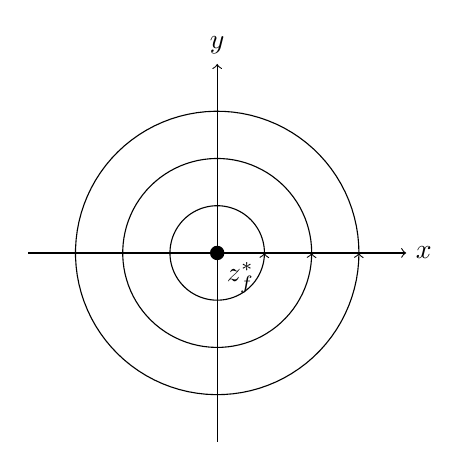
\begin{tikzpicture}[scale=1.2]
\draw[->] (-2,0) -- (2,0) node[right] {$x$};
\draw[->] (0,-2) -- (0,2) node[above] {$y$};

\foreach \r in {0.5,1,1.5}
{
  \draw[->,domain=0:360,samples=100]
  plot ({\r*cos(\x)}, {\r*sin(\x)});
}

\filldraw (0,0) circle (2pt) node[below right] {$z_f^{*}$};
\end{tikzpicture}
\caption{Schematic phase portrait of a stable spiral equilibrium.}
\label{fig:local_phase_portrait}
\end{figure}


黏性不会消灭拓扑结构，只会钝化它

 % 点源点汇流动拓扑、置换混合通风数学定义
\end{document}
